% -------------------------------------------------------------------------------------------------
%
%  Skeleton for theses at the Institute of Robotics and Intelligent Systems
%
% -------------------------------------------------------------------------------------------------
%
% FILENAME:   thesis.tex
%
% ABSTRACT:   main file for theses
%
% USAGE:      compile with PDFLaTeX
%
% EXCEPTIONS: -
%
% HISTORY:    written by Sascha A. Stoeter <stoeter@iris.ethz.ch>, www.stoeter.com, 02.06.2004
%             modified by Martin Probst, 18.08.2004
% -------------------------------------------------------------------------------------------------

\documentclass[12pt,a4paper]{article}
\usepackage{iristhesis}

% -------------------------------------------------------------------------------------------------
% Add needed packages. Some generally useful packages are listed for
% your convenience.
% -------------------------------------------------------------------------------------------------
\usepackage{subfigure}                          % enable the use of subfigures
%\usepackage{amssymb}
%\usepackage[bf]{caption}                       % must go after subfigure
\usepackage[thickspace,thinqspace]{SIunits}     
\usepackage{amsmath}
\usepackage{hyperref}                           % enable Hyperlinks in pdf/ps Docs
\usepackage{subfigure}
\usepackage{float}
\usepackage{pdfpages}

% -------------------------------------------------------------------------------------------------
% Some handy definition to simplify future markup changes
% -------------------------------------------------------------------------------------------------
\providecommand{\eg}{e.g.}
\providecommand{\etal}{\textit{et al.}}
\providecommand{\ie}{i.e.}


% -------------------------------------------------------------------------------------------------
% Select type of thesis
% -------------------------------------------------------------------------------------------------
%\renewcommand{\iristhesistype}{Semester}
%\renewcommand{\iristhesistype}{Diploma}
\renewcommand{\iristhesistype}{Master}
%\renewcommand{\iristhesistype}{Ph.D.}

% -------------------------------------------------------------------------------------------------
% Set names
% -------------------------------------------------------------------------------------------------
\renewcommand{\irisauthor}{Michel Heusser}
\renewcommand{\irisadviser}{Naveen Shamsudhin, Andrew Petruska}


% -------------------------------------------------------------------------------------------------
% Beginning of the main document body
% -------------------------------------------------------------------------------------------------
\begin{document}

% include all Bib-items even if they're not cited in the text
\nocite{*}

% This is the first part of the front matter. Pages appear unnumbered
% and the pages are not counted.

% Title page: set title and date preferably formatted according to
% ISO 8601
\iristitlepage{Magnetic Analysis of Ferromagnetic Helical Microstructures}{2015}


% This is the second part of the front matter. Pages appear with
% lowercase roman numbering. The first page number is 'i'.
\pagenumbering{roman}

% Dedication (optional)
\newpage

%\thispagestyle{empty}
\markright{}
\vspace*{\stretch{1}}
\begin{center}
    
\end{center}
\vspace*{\stretch{2}}

% Preface (optional)
\markright{Preface}
\section*{Preface}

First of all I would like to thank Naveen for his experienced advice who always managed to question the theories and for the very deep and interesting philosophic talks that not only managed to make me see things from a complete different angle but also kept me always motivated throughout my work.\\

Secondly I would like to thank Andrew for his very strong mathematical and computational skills that always made me push the boundaries and kept me well challenged. It seems that every time I felt there was no solution to a problem, he came with a life-changing answer, that made things look easy again.\\

 Finally I would like to thank the members of the department, specially George and my fellow students doing their thesis, for making my stay at the department a very rewarding and pleasant experience. I'm happy, not only to have learned a lot on my subject during this period, but also to have made good friends during it.
\newpage\mbox{}\newpage
% Abstract must not be longer than one page per language. English and
% German abstracts are mandatory.
\addcontentsline{toc}{section}{\protect\numberline{}{Abstract}}
\markright{Abstract}
\section*{Abstract}

This thesis starts by doing an extensive summary of existing and trending technologies in the field of microrobots for life sciences and puts emphasis on the benefits and potential of magnetic helical microrobots. It then proceeds to do an extensive mathematical analysis of the physics of magnetism and derives the formal definition of the very often used demagnetization matrices all the way from the Maxwell equations. From this formulation it is proven that, for soft-magnetic materials, one has to do the distinction between low and high fields, since the mathematics behind it are vastly different. The general high field case, where the magnetic body is saturated deals with surface integrals in three dimensions whereas the low field case deals with surface integral equations in three dimensions. Since the numerical solution to these problems are highly complex, magnetic simulations using FEM were used to assess the correctness of the numerical implementations of the solutions, as well as giving solutions where the numerical implementation was not possible. To be able to compare the real magnetization case of helices, nickel macrohelices were manually coiled and their magnetic properties were analyzed using a VSM setup which was then compared to the FEM simulated model.

%\addcontentsline{toc}{section}{\protect\numberline{}{Zusammenfassung}}
%\markright{Zusammenfassung}
%\section*{Zusammenfassung}

Kurzfassung der Arbeit.


% Table of contents
\newpage\mbox{}\newpage
\tableofcontents
\addtocontents{toc}{\vspace{.5\baselineskip}}


% List of tables
%\newpage
%\addcontentsline{toc}{section}{\protect\numberline{}{List of Tables}}
%\listoftables

% List of figures
\newpage
\addcontentsline{toc}{section}{\protect\numberline{}{List of Figures}}
\listoffigures

% Glossary kind of chapters
%\addcontentsline{toc}{section}{\protect\numberline{}{Notation}}
%\addtocontents{toc}{\vspace{.5\baselineskip}}
%\markright{Notation}
%\section*{Notation}
\label{s:Notation}

Explanation of symbols.



% This is the main part of the thesis. Pages appear with arabic numbering.


\pagenumbering{arabic}
% Main body
\newpage\mbox{}\newpage
%!TEX root = thesis.tex
\section{Introduction}
\label{s:Introduction}

\subsection{Microrobots}
From the research and advances in recent years in the area of miniature robots used in the medicine, it is not only clear that this industry always aims for minimally invasive procedures, but also, that a surgeon's technical skills can be delegated to appropriate technologies to improve precision and dexterity \cite{Hamdorf2000a}. Wireless microrobots could perform complicated to nearly-impossible tasks and have the potential of improvement various medicinal areas \cite{Nelson2010}. Although this is a field that is mostly under development, it has been advancing very fast in the past decade \cite{Joseph2005}, \cite{Nelson2010}.

The main advantage of wireless microrobots is the fact that many locations within the human body are available for intervention \cite{Kassim2006}, \cite{Menciassi2007}. With a dimension of only a few millimeters or less, microrobots enable intervension with little trauma in areas like the central nervous system, the urinary system, and the circulatory system \cite{Nelson2010}. However, there are several constraints on the development of their developments. As objects are scaled down, the generation and storage of power becomes more complicated. Also, volumetric effects like inertia and weight lose relevance in front of viscosity and electrostatics \cite{Purcell1977}, \cite{Wautelet2001}. The approaches taken at traditional robotics is therefore completely different as the one taken for  the design and fabrication of microrobots, which relies mostly on simulations for the design and experiments for the performance \cite{Nelson2010}.

Various challenges also appear within the environment in which microrobots are to operate. Changes in the size of cavities as well as the material properties of the medium and the movement of it (for example the pulsating flow of blood) are factors the microrobots have to be able to negotiate with \cite{Nelson2010}. Although from an engineering point of view, the design approach is different towards existing tethered methods (e.g. catheters) \cite{Haga2004}, the advantages are vast, ranging from improved maneuverability to reach of inaccessible internal locations.


\subsubsection{Basic functionalities}

Although microrobots could potentially be able to carry out complex operations autonomously in the future, real microrobots in a near future will be expected to carry simple operations, often supervised or operated by a clinician. In the following a list will be presented showing the simple medical tasks for microrobots that could be feasible in the near future \cite{Nelson2010}.
\begin{itemize}
\item \textbf{Targeted therapy}: \\ This is concerned with the localized delivery of different forms of substances and energies. Targeted drug delivery allows to deliver drugs with increased concentrations in a specific region, not only improving the efficiency of the drug but also reducing the risk of negative side effects \cite{Nelson2010}. Brachytherapy works similar to the targeted drug delivery, but instead of drugs it transports radioactive sources or seeds to unwanted cells (e.g. tumors) killing them with the radiated energy \cite{Devlin2007}, whereas hyperthermia and thermoablation aim for the same through localized application of heat (being powered by high-frequency magnetic fields and ultrasound) \cite{Andra2007}, \cite{Kobayashi2011}, \cite{Baronzio2009}. 


\item \textbf{Material removal}: \\ If the robots are big enough, special tools can be designed for the microrobots to accomplish their tasks, whereas if the robots are smaller, they themselves will be the tools.\cite{Nelson2010} The two methods of material removal are ablation and biopsy/excision. Ablation is the removal of material from a certain surface. Microrobots could use this method for the removal of unwanted deposits (e.g. fat) from walls of blood vessels, either through direct scraping or through ultrasonic waves  created by resonating structures \cite{Tabatabaei2011}. Biopsy (or excision) is the retrieval of tissue samples from the body for external analysis or, potentially in-vivo when combined with remote-sensing technologies \cite{Nelson2010}.

\item \textbf{Controllable structures}: \\ Here the microrobots act as static devices with controllable positions. The microrobots can act, for example, as a scaffold \cite{Zhang2005} which supports frames for nerve regeneration, organ development, or blood vessel regrowth. The microrobots can also be used as stents to keep passageways open (e.g. a clogged vessel) \cite{Ormiston2009}, \cite{Lally2006} or as occlusions to block them (e.g. a vessel that nourishes a tumor) \cite{Fabbrini2006}. Another application is to use the microrobots as implants or electrodes brain stimulation \cite{Polikov2005}.


\item \textbf{Telemetry}: This area refers to the transmission of information from a specific location within the body with the help of microrobots that would be normally very difficult to obtain\cite{Nelson2010}. This is possible through various methods like ultrasound, radio waves or visible light \cite{Jepsen2002}. The applications include remote sensing and marking. Remote sensing transmits a signal that could contain information about concentrations of interest (e.g. oxygen) or other relevant information like the presence of cancerous cells\cite{Nelson2010}. Marking is the transmission of the microrobot's position within the body. When both applications are combined the localization of otherwise unknown phenomena within the body is possible (e.g. bleeding). 

\end{itemize}
\subsubsection{Application Areas}
With the mentioned functionalities and a size small enough to reach difficult places throughout the body the application areas are the following.

\begin{itemize}
\item \textbf{The circulatory system}: \\
Its main parts are the heart and the vessels used to transport the blood throughout the body. The distance between the heart and a certain given blood vessel is what actually decides its function and its material properties, since the pressure of the pulsations become less significant for the smaller, more distant vessels \cite{Nelson2010}.

\begin{figure}[ht]
	\centering
  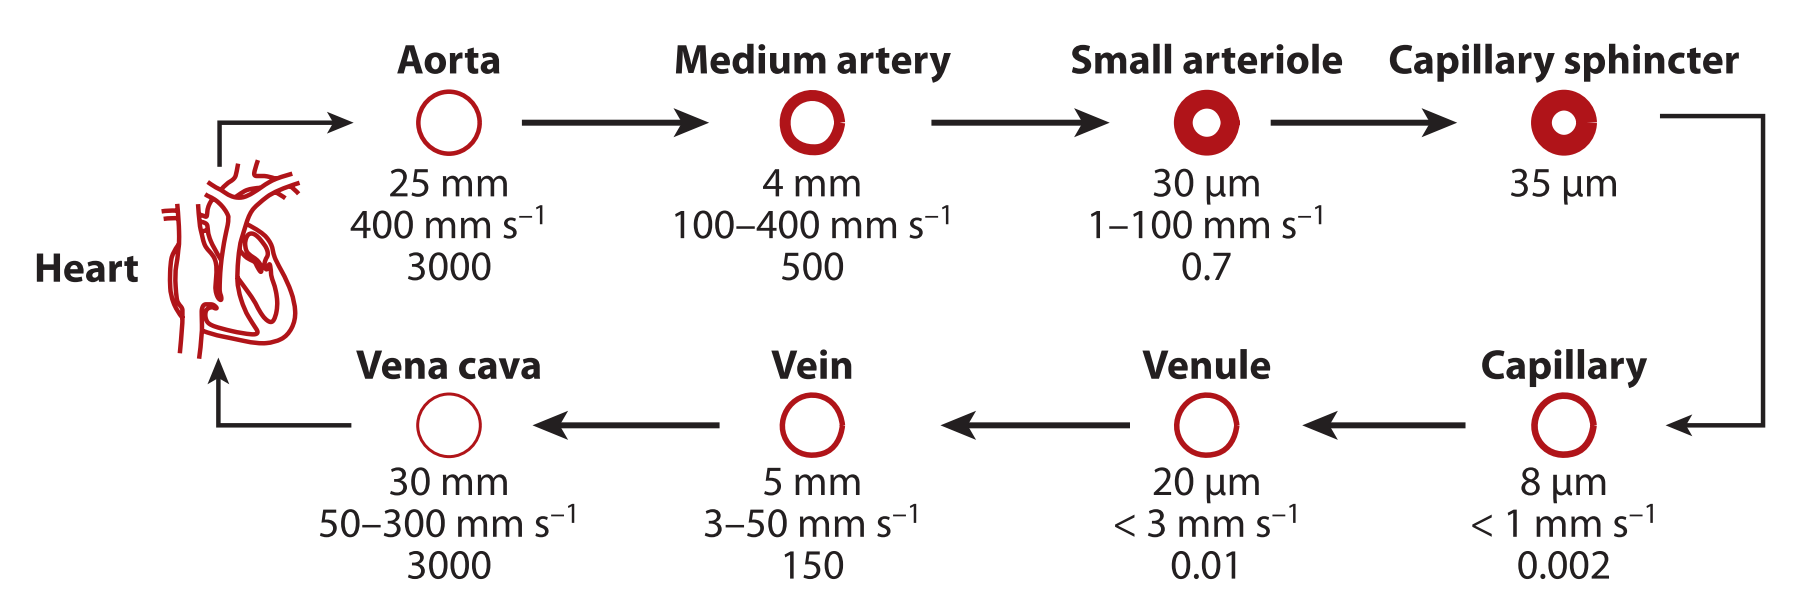
\includegraphics[width=1\textwidth]{Pictures/Bloodvessels.png}
	\caption{Vessels of the cardiovascular systems and their properties: inner diameter, average blood-flow velocity, and Reynolds number from \cite{berger1996}}
	\label{fig:veins}
\end{figure}

   In Figure \ref{fig:veins} we see the velocity and Reynolds number for the different vessel sizes. Altough blood has actually very similar intrinsic properties as those of water, the suspended blood cells create a much higher apparent viscosity as that from water. For a microrobot this could mean a very obstacle-filled working environment instead of an homogeneous liquid \cite{berger1996}. \\\\
Since almost every site within the body could be accessed through blood vessels, this could be the most important application for microrobots \cite{Nelson2010}. The most promising ones being drug delivery, removing plaque, destroying blood clots, stents or occlusions or even electrodes for electrophysiology. Some of the challenges microrobots could face tough, is the ability to swim against the flow \cite{Nelson2010}. Existing research (e.g. \cite{Cha2010}) has shown that this is indeed challenging, but possible.
\item \textbf{The central nervous system}: \\ It consists of the brain, the spinal cord, and the cerebrospinal fluid (Figure \ref{fig:nervoussystem}). The study \cite{Zaaroor2006} analyzed the geometrical and spatial characteristics of these for visualization of the spinal canal through endoscopy. These results can help set the design parameters for microrobots. Accessing the ventricles of the brain through the spine is actually possible and this would make microrobots potentially able to affect cancer therapy in the central nervous system and specifically within specific parts of the brain \cite{Nelson2010}. Injecting microrobots with a lumbar puncture would allow access to the brain for intervention, replacing invasive methods through the skull \cite{Purdy2003}. 
\begin{figure}[ht]
	\centering
  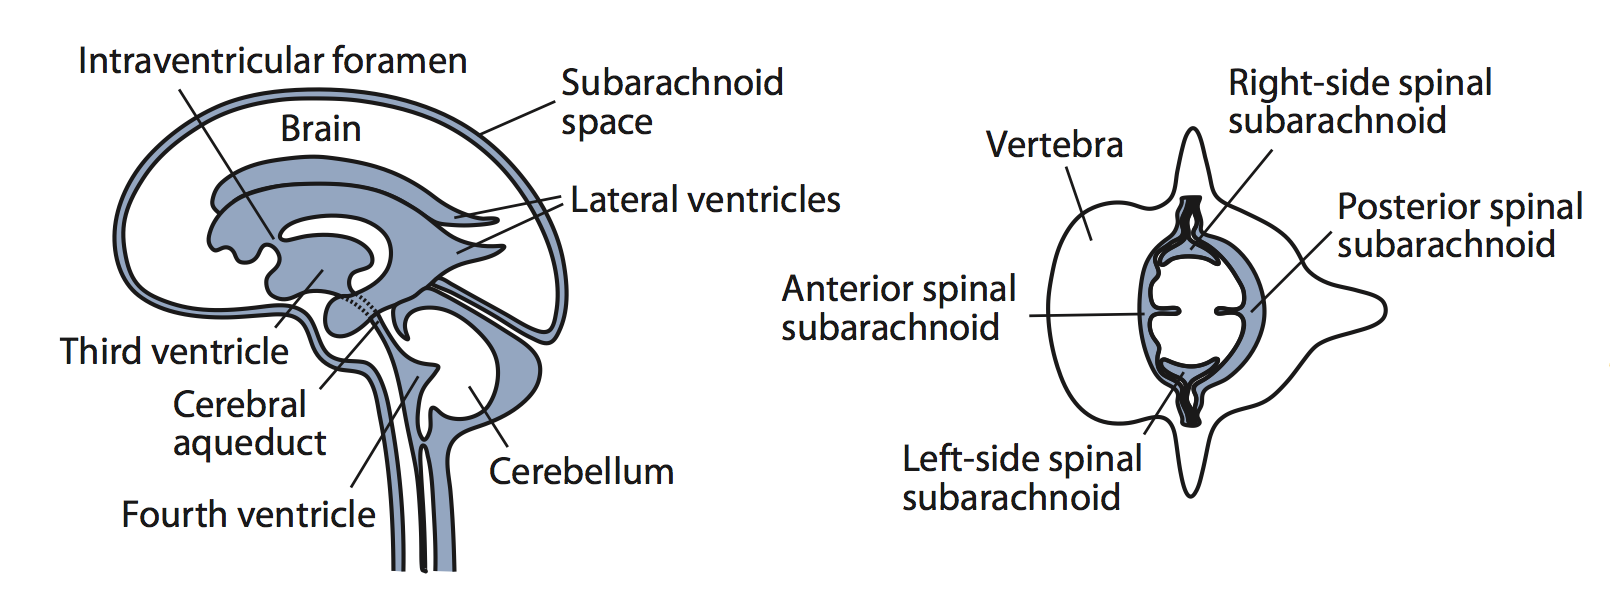
\includegraphics[width=1\textwidth]{Pictures/nervoussystem.png}
	\caption{The central nervous system, consisting of the brain and the spinal column \cite{Nelson2010}}
	\label{fig:nervoussystem}
\end{figure}
Other very important applications would be deep-brain simulation or neural prostheses, which normally would be nearly impossible since its hard reachability \cite{Nelson2010}.  Microrobots could even be used as permanent implants, but the brain's extremely delicate tissues would pose a challenge when designing them \cite{Nelson2010}.. Extensive research has been made in the field of wireless manipulation of magnetic seeds within the brain, specifically for hyperthermia methods. For more information refer to \cite{Molloy1990}.
\item \textbf{The urinary system and the prostate}: \\ This includes the kidneys, the bladder as well as the lumens connecting them and the urethra which connects the bladder to the exterior \cite{Nelson2010} (Figure \ref{fig:urinary}). 
\begin{figure}[ht]
	\centering
  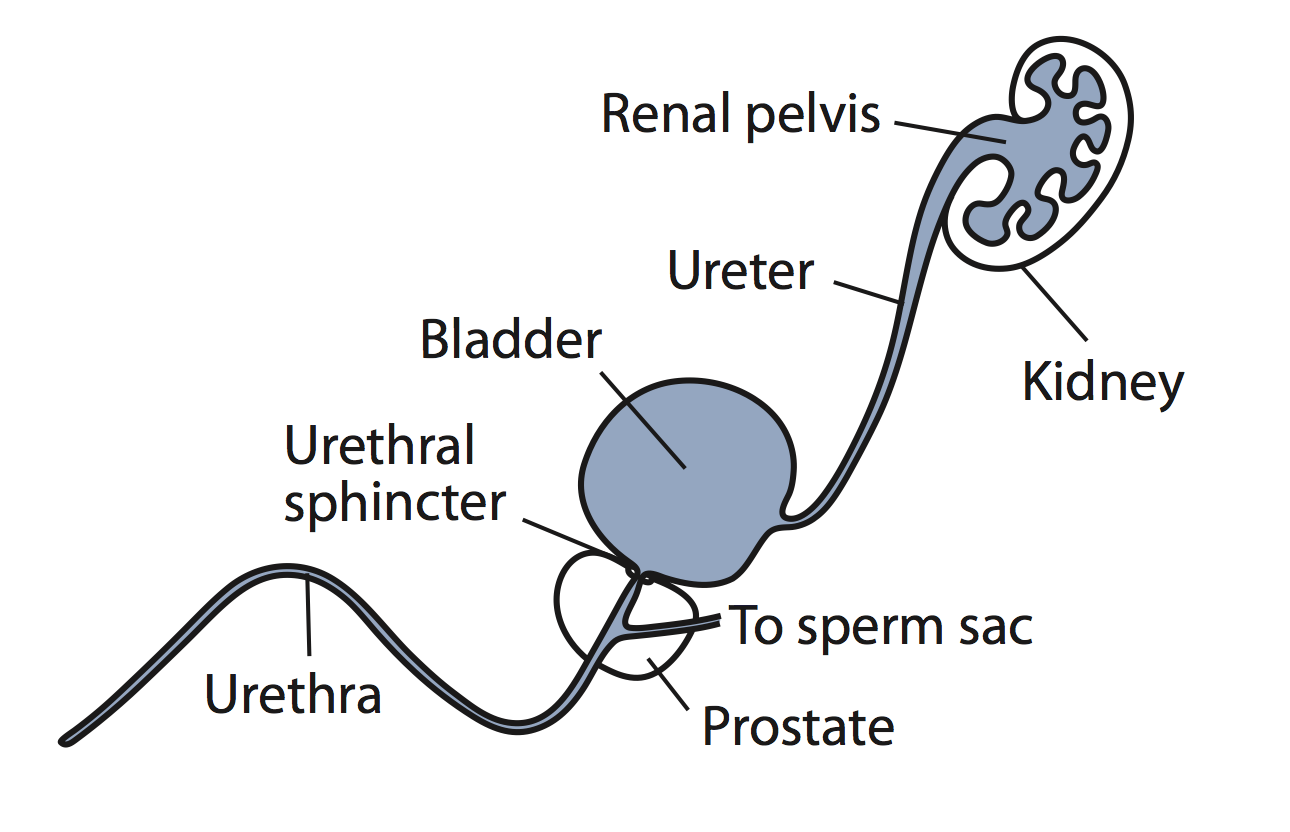
\includegraphics[width=0.5\textwidth]{Pictures/urinarysystem.png}
	\caption{The male urinary system as depicted in \cite{Nelson2010}}
	\label{fig:urinary}
\end{figure}

Microrobots operating in these areas could potentially improve the therapy of kidney stones without having to make any puncture on the kidneys which is usually related to cases of infection and blood loss \cite{Renner1999}. The methods used until now on tethered and implanted MEMS devises of urology \cite{Kristo2003} could be attached to wireless microrobots. Another possible application would be in the field of prostate cancer treatment. The most common methods used until know involve needle insertion through the perineum or through the colon, which involve the risk of damage to nerves and very complex maneuvers, respectively; microrobots would allow a minimally invasive access to the prostate through the urethra \cite{Nelson2010}. 
\item \textbf{The eye}: \\ The vitreous humor within eye is made of complex tissues that, although might be composed by mostly water, contain collagen fibrils that give viscoelastic properties and make it more of a soft tissue than a liquid \cite{Nelson2010}. The application of microrobots on the retina is where they have the most promising future, since it plays an essential role in the sight and it is very hard to access. Retinal surgery is strongly constrained by human performance \cite{Jagtap2004}, \cite{Balicki2010} and the forces needed are beyond human perception \cite{Gupta1999}, \cite{Iordachita2009} so the procedures are very risky. Microrobots would allow procedures without having to perform vicrectomy (removal of the vitreous humor) reducing the invasiveness and improving the results in the recovery \cite{Nelson2010}. The most promising application for microrobots would be diagnosis of retinal health as well as therapies for retinal vein occlusions and detached retinas, among others. There is extensive research on microrobots for intraocular procedures. For more information, refer e.g. to \cite{Yesin2006}, \cite{Ergeneman2008}, \cite{Ergeneman2008a}, \cite{Dogangil2008} and \cite{holligan2003}.
\item \textbf{The ear}:\\
The ear consists of the cochlea and the semicircular canals. It is then in this part, the inner ear, where microrobots have potential applications \cite{Nelson2010}. Through electrode implants within the cochlea that can stimulate the hearing nerve, hearing can be restored \cite{Cosetti2010}. However, the procedures are risky in terms of infections, trauma and even paralysis \cite{Stratigouleas2006} so there is still great potential for improvement through microrobots. Since the cochlear hair cells are respoinsible for natural hearing, there is extensive research around the stem-cell used for generation of these hairs. Microrobots could be used to transport and deliver the stem cells to the inner ear. For more information, refer to \cite{Parker2004} and \cite{Gunewardene2012}
\item \textbf{The fetus}: \\ Surgical procedures in a fetus can be very difficult since they are very invasive for both the mother and the fetus itself. However, open surgery can not only prevent death, but also have positive consequences for correcting impairments or malformations \cite{Flake2003}, \cite{Durkin2009}. Since they are lots of constraints in terms of dimensions and degrees of freedom of the tools that can be used, the use of microrobots have big potential of assisting these procedures \cite{Flake2003}, \cite{Berris2006}. A microrobot could perform tasks to treat cases of malformation through ablation or even act as a temporary tracheal occlusion against the pathological growth of the fetus's lungs \cite{Nelson2010}.
\end{itemize}

\subsection{Powering Microrobots}
The first challenge when designing microrobots is selecting a suitable source of power so that the locomotion can be achieved; compared to traditional robotics, there are many more limitations and constraints and we have to stick to the methods available to store, transmit and harvest power that are practically possible at the microscale \cite{Nelson2010}.

\subsubsection{Onboard scavenged power}
An feasible approach of providing a microrobot with power is with batteries; however, although these might be inexpensive, the amount energy they can provide scales with their volume, which makes them unsuitable \cite{Nelson2010}. Thin-film batteries, which use semiconductor technologies to operate, differ from traditional forms of batteries and could therefore be implemented on microrobots \cite{Nelson2010}. \\\\
Another relevant technology are MEMS-based generators. These have higher energy densities compared to batteries and traditional generators \cite{Jacobson2003}. There is also various studies that propose transducers that generate electrical energy out of different types of energy like chemical fuels, vibrations or temperature gradients \cite{DiSalvo1999}, \cite{kasap2006}. Biofuel cells, which operate at temperatures and pH similar to the ones found in the human body, would exploit the glucose and oxygen found in blood \cite{Bullen2006}, \cite{Barton2004}. Using muscle cells could be also used as actuators on micropillars \cite{Morishima2006}, cantilevers \cite{Kim2008} and other microscopic devices \cite{Xi2005}. Other possible methods of propulsion of microrobots is through the use of living microorganisms like magnetotactic bacteria, which respond to external magnetic fields \cite{Martel2009}. 

\subsubsection{Transmitted Power}
The alternative to power generation or storage implemented directly on the microrobot is the wireless transmission of energy to the device from an external source; the easiest method of doing this is using magnetic fields \cite{Nelson2010}. One method uses quasi-static or low-frequency magnetic fields that apply forces and torques directly on magnetic materials. The second method uses fluctuating magnetic fields to induce electricity. Studies \cite{Collins2002} and \cite{Siauve2003} show that, compared to electric fields, the magnetic permeability of the human body is practically the same as that in vacuum, which means that the body doesn't react to magnetic fields (i.e. magnetic transparency) and magnetic fields are therefore harmless. It is important to notice, that time varying fields do generate electrical field which could have as a consequence the cardiac fibrillation as a consequence of the stimulation of cardiac nerves. For more information about the risks and the recommended values of magnetic field and its time variation refer to \cite{Andra2007a}.

In the following, we will go in detail with the two mentioned methods of power transmission:

\begin{itemize}
\item \textbf{Induction}: \\ Using Faraday's Law of Induction we can understand this phenomenon:

\begin{equation}
V = -\frac{\textrm{d}}{\textrm{d}t}\int\limits_S \textbf{B}\cdot \textrm{d}\;\textbf{S}
\end{equation}
Here is $V$ the voltage created on a circuit by a time-varying flux of magnetic lines $\textbf{B}$ through the enclosed surface $\textbf{S}$. Usually the inducted electricity, which creates a magnetic field itself, has an effect on the circuit which created the original magnetic field $\textbf{B}$. The electricity which creates the original magnetic field is usually sinusoidal and the transfered power is optimizable (refer to \cite{bansal2006} and \cite{Theodoridis2005} for more details), but there are safety constraints that have to be taken in consideration. \\\\
Altough these methods are used in many devices \cite{Theodoridis2005}, \cite{Protection1998}, \cite{Lenaerts2007}, at the microscale there are design constraints when fabricating the small embedded coils. Also, the rectification of the voltage transmission becomes more important for microdevices since the voltage amplitudes decrease when the size decreases.

\item \textbf{Magnetic force and torque}: \\ Here the main principle is to generate mechanical energy directly on the microrobot out of magnetic fields. This is achieved by applying forces and torques directly on the magnetic materials of the microrobots. Equations ... and ... show how magnetic force and magnetic force are created from a magnetic field $\textbf{B}$:
\begin{equation}\label{eq:magdiptorqueint}
\textbf{F} = \int\limits_V(\textbf{M}\cdot\nabla)\textbf{B} \: \mathrm{d}V
\end{equation}
\begin{equation}\label{eq:magdiptorqueint}
\textbf{T} = \int\limits_V\textbf{M}\times\textbf{B}\: \mathrm{d}V + \int\limits_V \textbf{r}\times (\textbf{M}\cdot\nabla)\textbf{B} \: \mathrm{d}V
\end{equation}
where $V$ is the magnetic volume $\textbf{M}$ is the magnetization and $\textbf{r}$ is the distance from the gravity center of the body. For more details about the theory to magnetism please refer to Section (...). For small volumes, the external applied magnetic field can be modeled as uniform across the magnetic volume \cite{Nelson2010}. The magnetization usually varies throughout the body, but the average magnetization is used since the body is small \cite{Nelson2010}. Here, the strength of the forces and torques are proportional to the external field, the magnetization and the magnetic volume. \\\\
Ferromagnetic materials which exhibit a saturation magnetization and a hysteretic behavior, can be classified as either hard or soft, depending on how significant the hysteretical behavior is. Soft magnetic materials have no memory, and return to a non-magnetized state, when the applied field is removed, whereas hard magnetic materials exhibit a remanent magnetization after the applied field is no longer there \cite{Nelson2010}. \\\\
The magnetic effects on a certain body depends not only on its material properties, but also on its shape. Also, some directions within a certain shape are easier to magnetize than others. Understanding the fields that are required to control a permanent magnet wirelessly is relatively easy since the magnetization can be modeled as constant. However, for soft magnetic bodies much more complex analytical models are needed. Accurate models exist for real-time control of soft-magnetic axially symmetric bodies (beads, cylinders, ellipsoids) \cite{Abbott2007c} or bodies made out of thin planar parts \cite{Nagy2008}.\\

Soft magnetic bodies are easier to fabricate than permanent magnets, but most of the research deals with the modeling of soft magnetic bodies when they are saturated and the magnetization is near constant throughout the body. In cases where the soft magnetic body cannot be saturated, permanent magnets tend to be easier to deal with since there is little research on low-saturated cases \cite{Nelson2010}.
\end{itemize}

\subsection{Locomotion}
To be able to move a microrobot within the body energy should be transformed into movement. The material properties of the medium the robots are supposed to swim in, as well as the scale of the robots are very important. Choosing the right methods that best suit these properties is therefore essential. \\\\
The material properties of the medium are responsible for viscous forces, whereas the shape and size of the microrobot is responsible for the inertial forces. For a certain problem setting, we can calculate the corresponding Reynolds number, which is the ratio between viscous and inertial forces \cite{Purcell1977}. Since usually this number is used to compare similar geometries that only have different scales or swim in different mediums we only need a characteristic length $L$ within our geometry. Knowing the free stream velocity $v$ of the medium in relation to the robot, and the viscosity $\eta$ and $\rho$ of the medium, the ratio is calculated with the following formula:

\begin{equation}
\mathrm{Re} = \frac{\rho v L}{\eta}
\end{equation}

The Navier-Stokes equation describes the dynamics of any fluiddynamical phenomenon. If we nondimensionalize this equation we see the Reynolds numbers explicitly:

\begin{equation}
\frac{\rho v L}{\eta} \frac{\mathrm{d}}{\mathrm{d}t}\textbf{V} = - \nabla p + \nabla^2\textbf{V}
\end{equation}

Where $\textbf{V}$ is the velocity of the fluid and $p$ the pressure. If the fluid is very viscous, the free stream, the velocity very small, or the shape of the robot very small, the Reynolds number will be also very small, such that only viscous effects are of importance. The Navier-Stokes equation then simplifies then to: 

\begin{equation}
0 = - \nabla p + \nabla^2\textbf{V}
\end{equation}

Which is called a Stokes-Flow (for more details refer to  \cite{Purcell1977}). In this regime, turbulence will not happen and the flow pattern wont change much if the body moves slow or fast. A reciprocal movement (consisting of two movements that are the reverse of each other in time) will result in a negligible net movement. Usually the assumption of an open fluid is used in analytical models, but there are methods that take in consideration the effect of nearby walls \cite{Nelson2010}.\\\\
Many design methods for microrobots have been inspired by nature. Microorganisms have developed various ways of swimming at low Reynolds Number, which are completely different than the ones used by non-microscale animals \cite{Vogel2003}. Bacteria and other moving cells use non-reciprocal movement methods using different types of flagella that swim through the fluid causing propulsion. Three important methods are discussed in the following.


\subsubsection{Pulling with Magnetic Field Gradients}
This first method, is not very concerned with the details of form and locomotion of the microrobot. This principle uses the fact that, as seen in Equation (\ref{eq:magdiptorqueint}), a force can be generated out of the gradient of a magnetic field acting on a magnetized body, a method that has been used in medical application for a long time \cite{Gillies1994}. \\\\
Theres a variety of methods to create magnetic fields. The first method uses current controlled electromagnets that are positioned simultaneously. Successful implementation of this method in medical application has been seen \cite{Grady1990}.  A study \cite{Yesin2006} was also made with the overlapping of two uniform fields created by a pair of coils, then the gradient is created with a second pair of coils. Through positioning of these coils, the magnetic microrobot can be manipulated. The second method uses stationary electromagnets that are also current-controlled. In \cite{Meeker1996} three pairs of coils were positioned orthogonally in a helmet-like fashion to control the magnetic field within the human head. Another possibility is to control ferromagnetic beads with the coils used in an MRI system \cite{Mathieu2006}. The third method uses permanent magnets which is used to position magnetic-tip catheters \cite{Stereotaxis2008}. \\\\
References \cite{Nagy2008} and \cite{Abbott2007c} show analytical models for the magnetic force and torque on soft axially symmetric bodies and assembled-MEMS bodies. The advantage of these over magnetic beads is the ability to magnetize easily thanks to their strong shape anisotropy. Their shape allows them to saturate with much lower applied fields than with the beads \cite{Nagy2008}, \cite{Yesin2006}, which makes wireless control more feasible. \\\\
Locomotion achieved through the force generated by magnetic field gradients has no analogy in nature. Which could mean that is a method more effective than the mechanisms nature has developed through natural selection. It has been shown, however, that microrobots that use elastic-tail or helical propulsion are much more promising for medical applications \cite{Abbott2010}. This is because the decrease in maximum speed and force generated through gradients decay much faster when scaling down than with helical and elastic-tail propulsion and also because its easier to project magnetic fields than gradients over long distances. 

\subsubsection{Traveling-Wave Propulsion}
This method is inspired by the eukaryotic flagella. It works by the principle of traveling waves along a flexible tail, which is a non-reciprocal movement and therefore suitable for low Reynolds numbers. Although it may be a very effective movement \cite{Behkam2006}, creating this type of movement in a microrobot, as well as its control and fabrication is very difficult.\\\\
In \cite{Kosa2007} a method of constructing this propeller through piezoelectric materials is proposed. This consists of using two layers of piezoelectric actuators that make the propeller bend when one is put in tension and the other one in compression. Through alternating this mechanism one can simulate a traveling wave. The larger the number of piezoelectric actuators the better does the movement approach the one of the flagella. \\\\
Another method uses both magnetic fields and electrical power \cite{Kosa2008}. Different current-controlled coils are distributed throughout the propeller. Magnetic fields are created with the mentioned coils, which will try to align with an external applied field. Through controlling of the currents in the coils, a traveling wave can be created. This has the potential of being powered by an MRI system.\\\\
When using an elastic tail, one can imitate quite accurately the movement of the flagella only with a single actuator (acting like a whip). The disadvantage is that the efficiency is not as high as with the methods presented above. The main problems that can arise with propellers of the types mentioned here is that a very short rigid propeller, will do a reciprocal motion, whereas a long one, although approaching a perfect traveling wave, will generate a much higher drag force \cite{Nelson2010}. \\\\
The final method of propulsion is through the implementation of a chain of paramagnetic beads to form an artificial flagellum \cite{Dreyfus2005a}. An oscillating field can induce then a wave motion in the chain. Additional analysis of this swimming method has been analyzed in detail in \cite{Roper2006}, \cite{Gauger2006} and \cite{Roper2008}. The drawback here is that a body is needed where the chain has to be connected to, otherwise the drag of the flagellum creates a zero net movement.  
\subsubsection{Helical Propulsion}
We arrive to the final and for this thesis, the most important type of propulsion. This method is inspired by bacterial flagella, which use a rotor-like movement to create a helical movement out of a passive straight elastic flagellum. Scaling down a similar mechanism is extremely difficult, but a simplification is possible. Since we want to go deep in detail with this type of locomotion and its powering mechanism. We will dedicate a new section two it.

\subsection{Chiral magnetic nanomotors}
The propulsion of magnetic nanomotors with a chiral shape by a rotating magnetic field is the focus of modern biomedical applications. It relies on the interactions of the magnetic and dynamical characteristics and interactions of the system. The interest on them mainly relies on the fact that they are bio-inspired, remotely controlled and can be navigated in vivo to a specific location. They show immense potential in biomedical applications since they allow fuel-free and contact-free propulsion without changing the chemical properties in the medium and environment. \cite{Morozov2014a}. \\\\
Various research studies have proved experimentally possible to control magnetic helical propellers using rotating magnetic fields made out of ferro-magnetic, soft-magnetic materials \cite{Zhang2009}, \cite{Zhang2009a} or permanent-magnetic materials \cite{Honda1996}, \cite{Ghost2009} in many sizes including the microscale. A big advantage ist that the use of weak magnetic fields can be used to achieve the locomotion of ferromagnetic nanomotors \cite{Solovev2009}, \cite{Ghosh2009}, \cite{Wang2013}. These have to be previously magnetized by strong magnetic fields, creating a remanent magnetization when the field is removed and remains despite the presence of said weak rotating magnetic field. The velocities achieved by this mechanism are up to five orders of magnitude higher than those achieved using magnetic field gradients \cite{Nelson2010}. \\\\
Independently of the magnetic material used and the energy transfer to the helical propeller, there exist different ways of fabricating them. It can range from strips made out of different layers that obtain the helical form due to internal stresses \cite{Zhang2009}, \cite{Zhang2009a} to a wire being brought to a helical form \cite{Honda1996}. It has also been proved \cite{Purcell1977} that the efficiency of the helical structure does not depend on the cross-section of the helix. Also, the helical non-reciprocal form of the helix, allows us to revert the direction of motion so that both pulling and pushing actions are possible. \\\\
Although the preferred method would be using a rigid structure, one could use a fiber that twists up into the helix structure that stays until the torsion is removed, but this may result in less controllability towards rigid helices as well as the inability to perform a pulling motion, reversing the rotating direction (See Figure \ref{fig:rotatingflagella}) \cite{Nelson2010}. \\

\begin{figure}[ht]
	\centering
  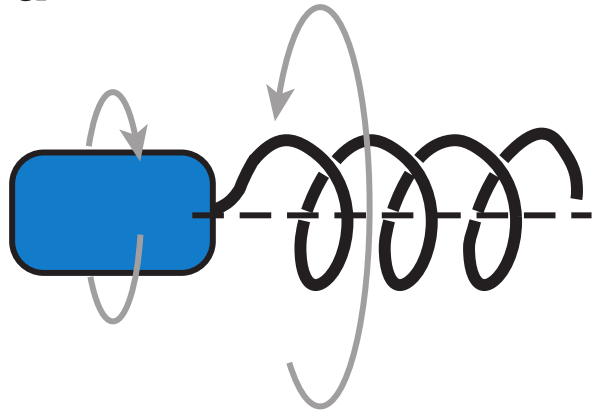
\includegraphics[width=0.5\textwidth]{Pictures/rotatingflagella.png}
	\caption{A rotary actuator turns the propeller and the body counterrotates as shown in \cite{Nelson2010}}
	\label{fig:rotatingflagella}
\end{figure}

Apart from the mentioned propulsion strategies mentioned above (rigid and non-rigid helical propulsion) there exist two other strategies for moving through lumens and soft tissue. The first one resembles more a crawling than a swimming motion. The second one involves a screw-shaped microrobot that literally screws through the medium advancing only one pitch height of the helix for one turn of it. For more information about these, please refer to \cite{Sendoh2003} and \cite{Ikeuchi1997}. In the following we will go more in detail on the methods of fabrication of these helices. 

\subsubsection{Fabrication}
The production of these structures can be achieved by various fabrication methods like ''top-down'' approach \cite{Zhang2009}, delamination of magnetic stripes \cite{Smith2011}, , glancing angle deposition \cite{Ghosh2009} as well as direct laser writing with vapor deposition \cite{Tottori2012} achieving not only the fabrication of ferromagnetic structures in the microscale but also in the nanoscale \cite{Schamel2014}.


\subsubsection{Dynamic Properties}
Independently of the strategy used from the above methods for rigid propellers we can generalize the dynamics for a movement along the helix axis. For low Reynolds number, there are linear relations between the torques and forces, and velocities, and rotation \cite{Tottori2012}, \cite{Peyer2013}, \cite{Peyer2010}, \cite{Rodenborn2013}, \cite{Behkam2006} and \cite{Abbott2010}:\\

When the torque is obtained by rotation of a magnetic field, the propulsion is fundamentally controlled by the rotation frequency of the field. The microrobot reaches an equilibrium shift of phase rotating in sync with the magnetic field . This way, the magnetic torque is in perfect balance with the torque generated by the drag forces of the medium. \\


\begin{equation}\label{eq:LinearSpeed1}
\left(\begin{array}{c}
v \\
\omega \\
\end{array}\right) =
\left[\begin{array}{cc}
a & b \\
c & d \\
\end{array}\right] \left(\begin{array}{c}
f \\
\tau \\
\end{array}\right)
\end{equation}

FIGURE 5a

It makes sense to rearrange Equation \ref{eq:LinearSpeed1}  such that the input variables are the force applied on the robot $f$ as well as the rotation frequency $\omega$ as follows:

\begin{equation}
\left(\begin{array}{c}
v \\
\tau \\
\end{array}\right) =
\left[\begin{array}{cc}
A & B \\
-B & C \\
\end{array}\right] \left(\begin{array}{c}
f \\
\omega \\
\end{array}\right)
\end{equation}

In Figure \ref{fig:LinearSpeed1}  we see the forward velocity growing linearly with the frequency until the so-called ''step-out'' frequency is reached (consistent with Equation \ref{eq:LinearSpeed1}). This is the frequency where the magnetic torque is no longer big enough to keep the structure rotating in sync with the magnetic field. Here the velocity starts decreasing significantly. Recent studies  \cite{Peyer2013}, \cite{Morozov2014} and \cite{Morozov2014a} has shown experimentally this behavior. \\

\begin{figure}[ht]
	\centering
  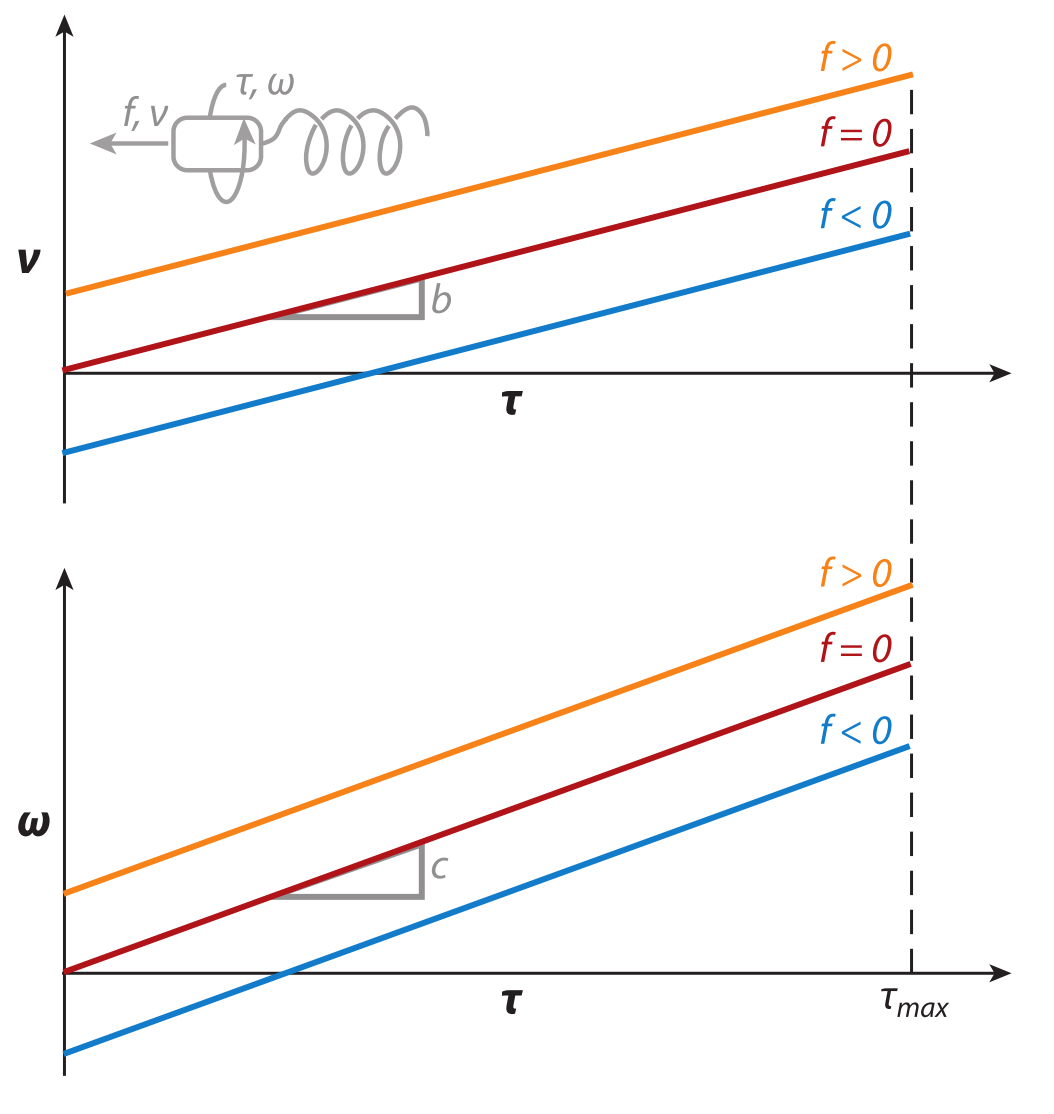
\includegraphics[width=0.7\textwidth]{Pictures/LinearSpeed1.png}
	\caption{Dynamic behaviour of helical-motors as shown in \cite{Nelson2010}}
	\label{fig:LinearSpeed1}
\end{figure}

Rodenborn did an analysis in \cite{Rodenborn2013} using the above linear model to find out the dynamic parameters $a,b,c,$ and $d$ using macroscopic swimmers in a highly viscous fluid (keeping the Reynolds number very small) and measuring the relevant dynamic variables. Comparatively numerical simulations where performed using resistive force theory of Gray and Hancock, and Lighthill, slender body theories (Lighthill and Johnson) as well as the Stokeslet numerical method. In this analysis the experimental results differ significantly from the predictions of the models used by resistive force theory, whereas the slender body and Stokeslet analyses agree with them (Figure \ref{fig:Rodenborn2013}). \\

\begin{figure}[ht]
	\centering
  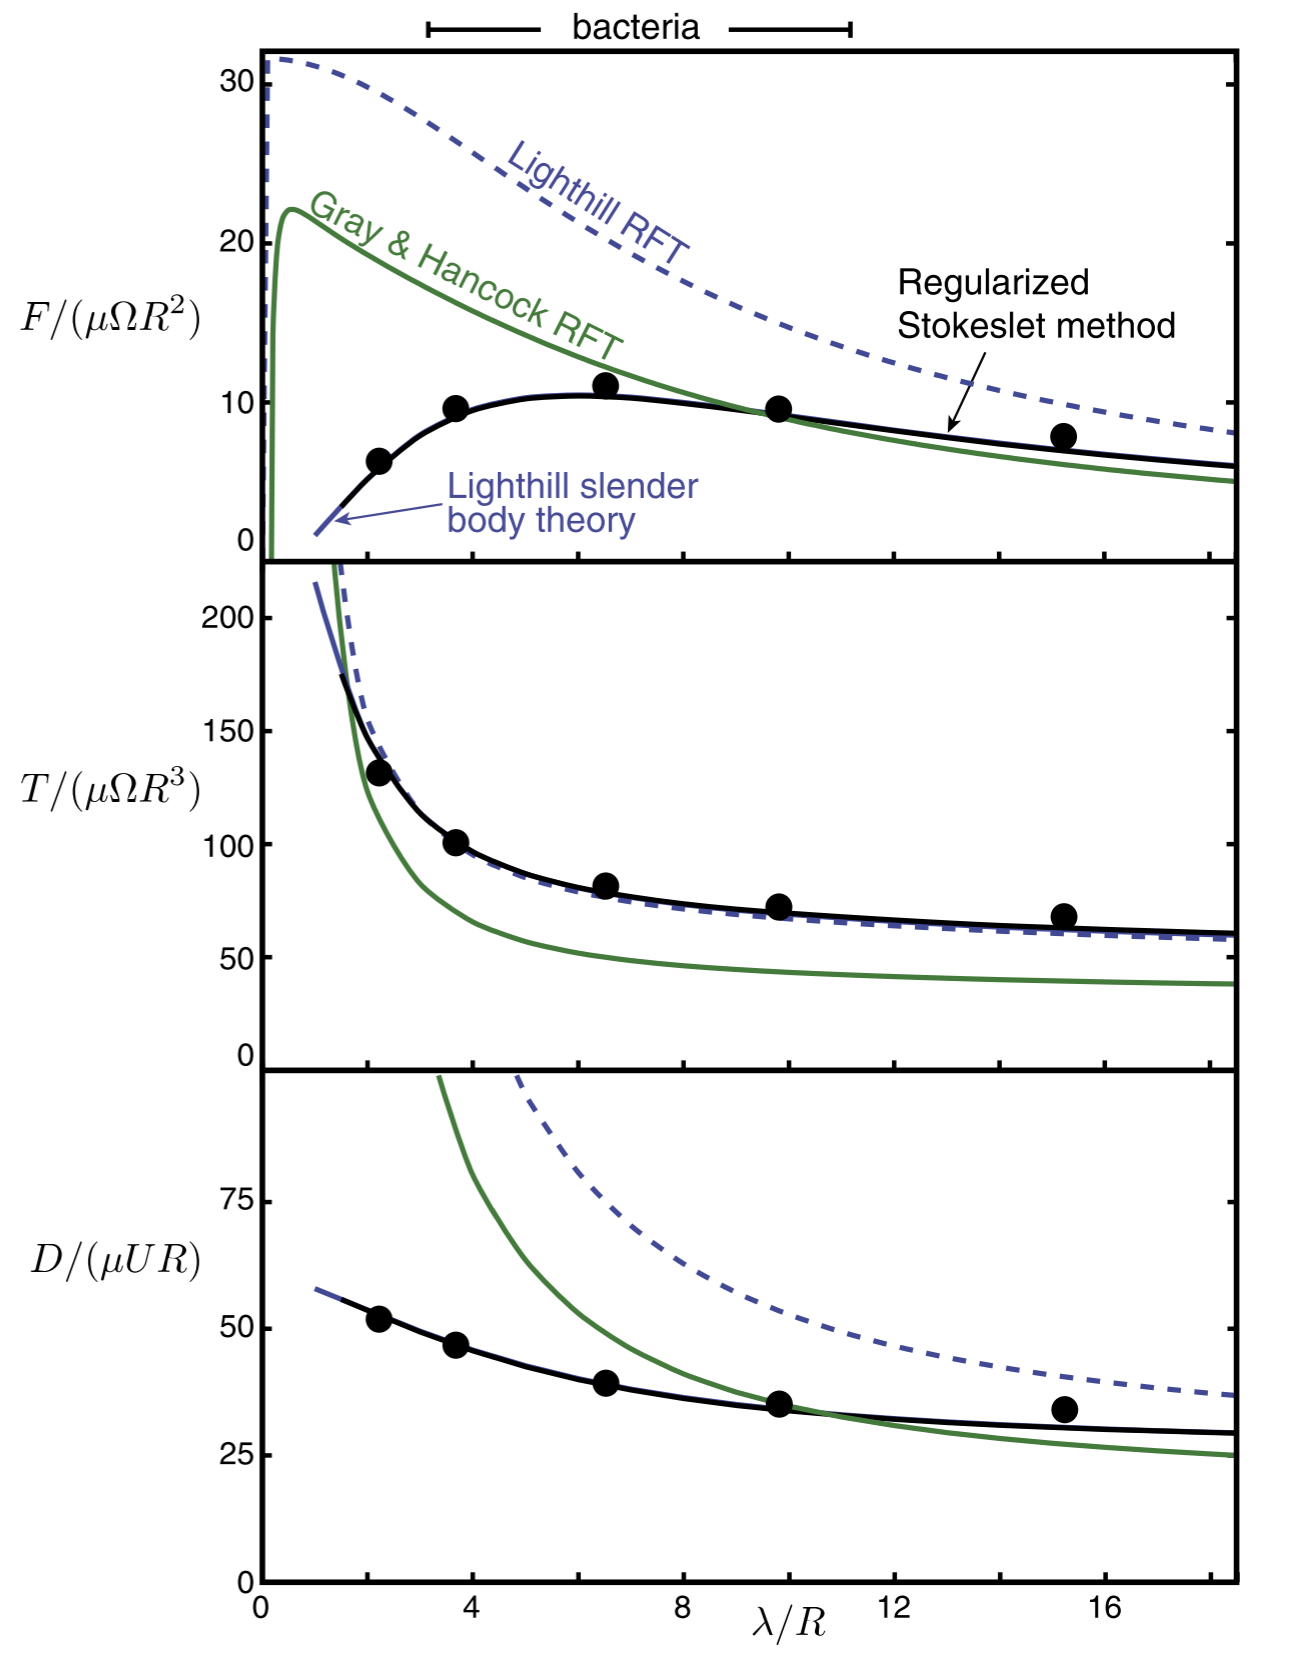
\includegraphics[width=0.7\textwidth]{Pictures/Rodenborn2013.png}
	\caption{Dynamic measurements (Thrust, torque and drag) compared to Resistive Force Theory model, Slender Body model and Stokeslet analysis for helical flagella as a function of pitch-to-radius ratio as shown in \cite{Rodenborn2013}}
	\label{fig:Rodenborn2013}
\end{figure}

\cite{Morozov2014} analyzed the different regimes when it comes to orientation and propulsion depending of the actuation frecuency. The theoretical predictions agree accurately with the available experimental data. Although in Figure \ref{fig:LinearSpeed1} the relation between propulsion speed and frequency is linear, it only holds when the helix is performing a perfect rotation along the helix axis. \cite{Morozov2014} includes the fact that a wobbling/tumbling movement is first reached until the movement stabilizes to a perfect rotation along the axis. This creates nonlinearities in the model. In Figure \ref{fig:Morozov2014a} we see this behavior. \\

\begin{figure}[ht]
	\centering
  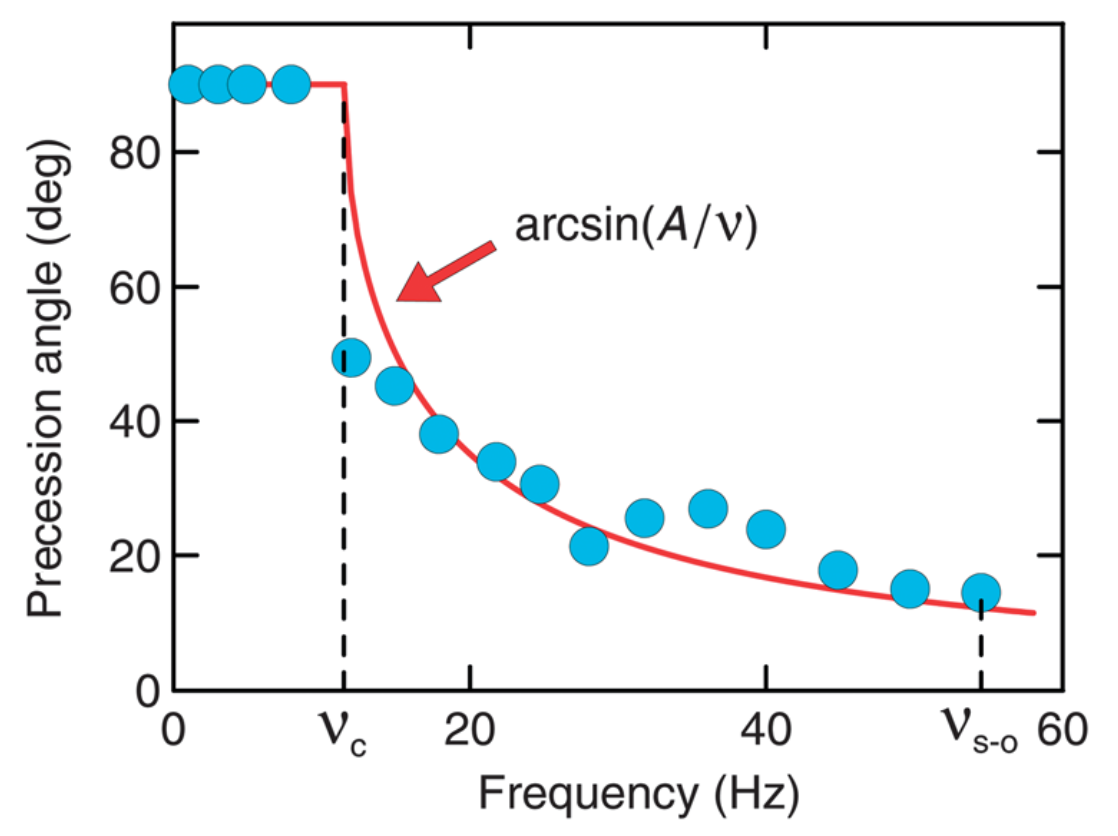
\includegraphics[width=0.7\textwidth]{Pictures/Morozov2014a.png}
	\caption{Experimental results of propulsion as a function of frequency as shown in \cite{Morozov2014}}
	\label{fig:Morozov2014a}
\end{figure}

Figure \ref{fig:Morozov2014b} on the other hand, shows how the precession angle stabilizes towards zero with higher frequencies (before the step out frequency).\\

\begin{figure}[ht]
	\centering
  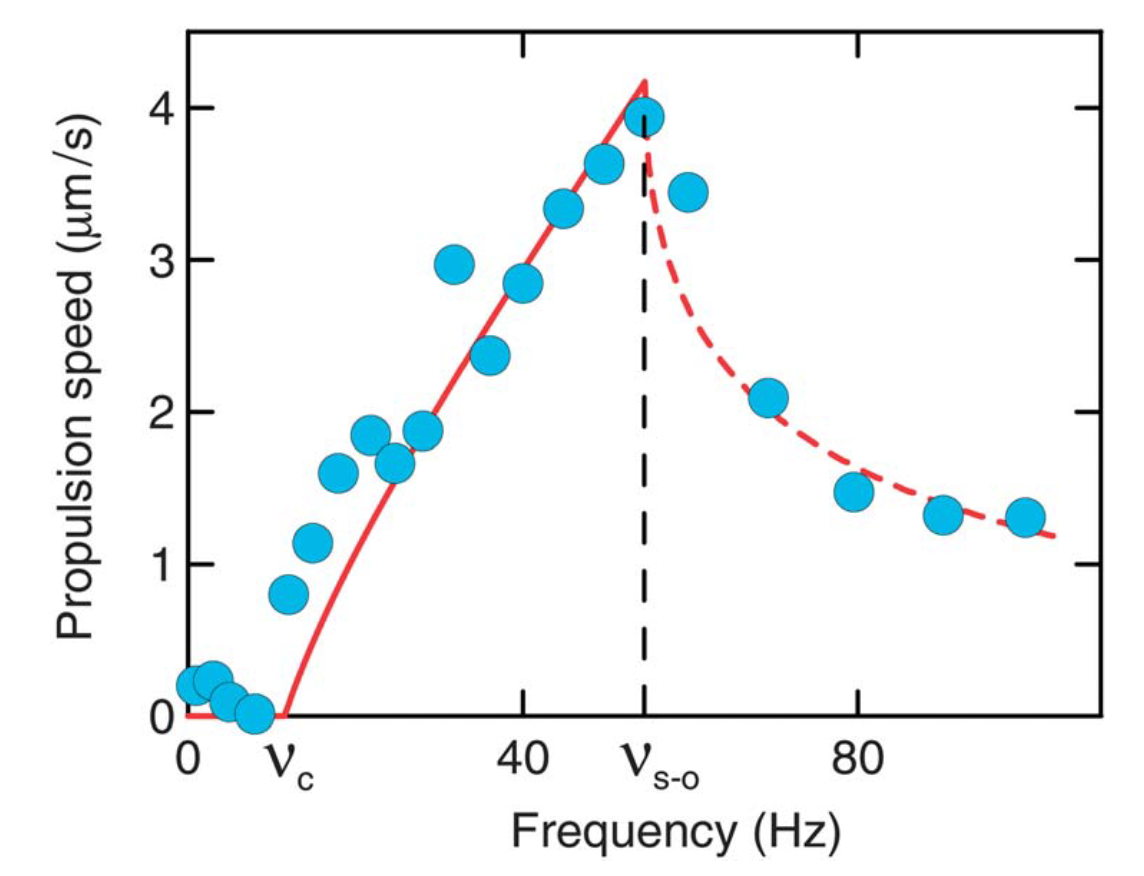
\includegraphics[width=0.7\textwidth]{Pictures/Morozov2014b.png}
	\caption{Experimental results of precession angles as a function of frequency as depicted in \cite{Morozov2014}}
	\label{fig:Morozov2014b}
\end{figure}

\subsubsection{Magnetic Properties}

As it was mentioned above. In order to achieve a more optimal propulsion, the orientation of the helix towards the axis of the rotating magnetic field (precession angle) plays an important role. Clearly the magnetic properties of the helix are crucial, specially how the body itself magnetizes in the presence of an applied field. Several studies go into this topic. \cite{Abbott2007} deals with soft-magnetic axial symmetric bodies and actually mentions that magnetization with a low applied field completely differs from a magnetization with a high applied field. \cite{Morozov2014a} analyses the alienation of the helix with a given magnetization on a given applied field. \cite{Sheka2015} goes in depth with the details of the magnetization of a helix in presence of a applied field and the effects that arise due to the curvature of the geometry.







\newpage\mbox{}\newpage
%!TEX root = thesis.tex

\section{Scope and Framework}

Various existing studies that go in depth with magnetization of different ferromagnetic or soft-magnetic structures (not necessarily helices) seem not to draw a line between high (saturated) magnetizations and low (unsaturated) magnetization of the magnetic structures and seem to use the same shape-factor $N$ of a structure disregarding of the magnetization grade. The main scope of this thesis will be to analyze the magnetization properties of a set of polycrystalline ferromagnetic helices with different coiling grades in the microscale in presence of high applied fields and low applied fields. First we will set-up the theory coming from basic physical principles (Maxwell Equations) and we will derive all the relevant parameters, in particular, the demagnetization factor $N$. To obtain theoretical results we will use a of FEM simulations using COMSOL and we will try to match them through implementation of the theoretical results with Matlab. As a final step, we will run experiments on macroscale ferromagnetic polycrystalline helices on a VSM machine and will compare the results with their modeling in COMSOL. 

\subsection{Helices}

In the previous chapter we derived the H-Field created by a certain magnetized body. In this section we will use the solution derived there and derive the demagnetization tensor as a variable of high technical importance, that will help us understand magnetization in a more intuitive way. After that, we will derive the formulas that describe the framework we we're working with on this project.\\

The set of helices that will be used here for analysis, are the ones existing experimental data has been found and is consistent with the research within this laboratory. The detailed measurements of these can be found in the Appendix, but we will refer them H1 to H10 as a measure for elongation (See Figure \ref{fig:Helices}). They all have the same wire thickness and magnetic volume (length of the wire) and only the pitch size, as well as the helix diameter, will be a variable parameter (encapsulated by the index).

\begin{figure}[ht]
	\centering
  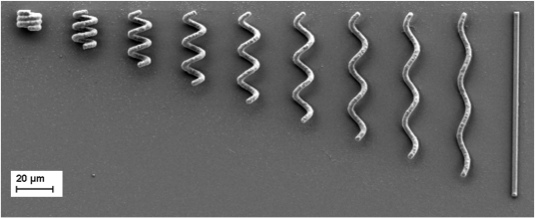
\includegraphics[width=1\textwidth]{Pictures/Helices.png}
	\caption{Helices H1 to H10}
	\label{fig:Helices}
\end{figure}


\subsection{Magnetic Properties of our Materials}

For the helices the materials used is polycrystalline Nickel, which displays a ferromagnetic behavior. As we said in the previous chapter, the type of material, and how it magnetizes is given by the relation between the applied field and the magnetization: $\textbf{M} = f(\textbf{H})$. In the case of ferromagnetic materials this is given by the magnetization loop for that specific material.

This $f(\cdot)$ is not a proper function, but more a complex mathematical construct that takes in account the magnetic history of the material showing a hysteresis loop. We will later show that the materials used in this project show a very narrow hysteresis loop so that it can be modeled as a function that saturates at high applied magnetic fields. In this case we can write the relation in the following way:

\begin{equation}
\textbf{M} = \chi_m(\textbf{H})\;\textbf{H}
\end{equation}

In general $\chi_m(\textbf{H})$ is an H-dependent tensor, but Nickel is actually isotropic, such that the direction doesn't matter. The tensor can be then simplified to a scalar function\footnote{in this case the scalar can always be written in tensor notation as the identity matrix times the scalar}

The reason for writing it this way is to have a nice analogy to the linear case, where $\chi_m$ is a constant tensor.

For more information about the details of the topic refer to \cite{Cullity2009}





\newpage\mbox{}\newpage
%!TEX root = thesis.tex
\section{Background Theory}
\label{s:Theory}

For the explanation of the theory used in this thesis, I based myself in \cite{Griffiths2005} and \cite{leuchtmann2005}.

The theory of electromagnetism is fully described by the Maxwell Equations (with their initial and boundary conditions) and the Lorentz force law. 
\begin{subequations}
\begin{equation}\label{eq:mx1}
\nabla \cdot \textbf{E} = \frac{\rho}{\epsilon_0}
\end{equation}
\begin{equation}\label{eq:mx2}
\nabla \times \textbf{E} = -\frac{\partial\textbf{B}}{\partial{t}}
\end{equation}
\begin{equation}\label{eq:mx3}
\nabla \cdot \textbf{B} = 0
\end{equation}
\begin{equation}\label{eq:mx4}
\nabla \times \textbf{B} = \mu_0(\textbf{J} + \epsilon_0\frac{\partial\textbf{E}}{\partial t})
\end{equation}
\end{subequations}

and

\begin{equation}\label{eq:lorentz}
\textbf{F} = Q(\textbf{E}+\textbf{v}\times\textbf{B})
\end{equation}

Although the interest in this thesis is only to analyze magnetic properties, I'll explain the analogies to the electrical properties since the mathematics in magnetostatics and electrostatics are very similar and much more intuitive in the latter.\\

I will  clarify the assumptions taken (macroscopic fields) and the effect of materials on the magnetic and electric fields.

\subsection{Electrostatics}

In the field of electrostatics, there are by definition no moving charges.  Equations (\ref{eq:mx1}) and (\ref{eq:mx4}) simplify then to (we're only interested in electric fields):

\begin{subequations}
\begin{equation}\label{eq:mx1st}
\nabla \cdot \textbf{E} = \frac{\rho}{\epsilon_0}
\end{equation}
\begin{equation}\label{eq:mx2st}
\nabla \times \textbf{E} = 0
\end{equation}
\end{subequations}
with the boundary condition:
\begin{equation}\label{eq:mx12stbc}
\lim_{||\textbf{r}||  \rightarrow \infty} \textbf{E} =0
\end{equation}

This formulation describes the electrical field in any situation (macroscopic or microscopic).\\

Equation (\ref{eq:mx1st}) states that the source of an electrical field is a charge. Since this is a differential description, the charge has to be given as a charge volume density $\rho$. This doesn't necessarily make the assumption, that the charges are rather spread as a continuum over space. We can still construct a discrete microscopic model (e.g. a crystal) by using Dirac delta functions to represent point charges.\\

Equation (\ref{eq:mx2st}) gives the property of $\textbf{E}$ being a conservative vector field. In other words since the following holds:

\begin{equation}
\nabla\times(-\nabla\phi) = -\nabla\times\nabla\phi =0 \qquad \forall \phi
\end{equation}

equation (\ref{eq:mx2st}) states that there exists in fact a scalar function $\phi$ such that:

\begin{equation}
\textbf{E} = -\nabla\phi
\end{equation}

This function will be called "electric potential function"  and will make some problems easier to solve, since we only have to find the potential function in order to have all the information regarding the electrical field. Since the electrical field is essentially a force (per charge) field, the potential function will have a nice physical meaning, namely energy (per charge).

\subsubsection{Influence of Materials}

Theoretically, to obtain the electrical field in the space nothing else is needed than equations (\ref{eq:mx1st}), (\ref{eq:mx2st}) and (\ref{eq:mx12stbc}). However when dealing with real materials, the complexity of the problem increases dramatically needing a mathematical model that allows us to deal with it more easily. This is the case for non-conducting materials (also called dielectric materials).\\

We have learned that only charges have an effect on the electrical field. Although an uncharged electric material is made of atoms, which have negatively charged electrons and positively charged protons, the material itself won't produce any net electrical field since the charges' individual electrical fields cancel each other out. However, when said material is put inside of an existing electrical field, the charges inside of the atoms are pushed out of their positions such that their electrical fields don't cancel each other out and an actual contribution to the total electrical field is created. This shifting effect is called polarization and is characterized by the dipole moment $\textbf{p} = q\textbf{d}$, which has the information about the charge $q$ as well as the shift (and its direction) $\textbf{d}$.\\

In the end, this dipole moment is the one that is directly connected to the force and torque acting on the analysed body (in this case an atom) in the following way:
\begin{subequations}
\begin{equation}\label{eq:elecdiptorque}
\textbf{T}_\text{elec} = \textbf{p}\times\textbf{E}
\end{equation}
\begin{equation}\label{eq:elecdiptorque}
\textbf{F}_\text{elec} = (\textbf{p}\cdot\nabla)\textbf{E}
\end{equation}
\end{subequations}

However, we're interested in using a macroscopic model that doesn't require us to deal the dipole moment of every polarized atom. For this we define a new macroscopic variable, that describes the dipole density assuming we're at a continuum, called polarization $\textbf{P}$. With:

\begin{equation}
\int\limits_V \textbf{P} \;\mathrm{d}^3r = \textbf{p}
\end{equation}

Since we're in a macroscopic continuum and the shifting of the charges $\textbf{d}$ is very small, we can use the potential generated of a dipole $\textbf{p}$ (taken as a point at the origin)

\begin{equation}
\phi_{dip}(\textbf{r}) = \frac{1}{4\pi\epsilon_0} \frac{\textbf{r}\cdot\textbf{p}}{r^3}
\end{equation} 

and use its relation to the polarization $\textbf{P}$:

\begin{equation}\label{eq:dipolpot}
 \phi(\textbf{r})=\frac{1}{4\pi\epsilon_0}\int\limits_V \frac{(\textbf{r}-\textbf{r}')}{|\textbf{r}-\textbf{r}'|^3}\cdot\textbf{P}(\textbf{r}')\; \mathrm{d}^3r'
\end{equation} 

using mathematical manipulations we arrive at the following:

\begin{equation}\label{eq:dipolpotexp}
 \phi(\textbf{r}) = \frac{1}{4\pi\epsilon_0} \oint\limits_{\partial V} \frac{1}{|\textbf{r}-\textbf{r}'|}(\textbf{P}\cdot \textbf{n}')\;\mathrm{d}^2r' - \frac{1}{4\pi\epsilon_0} \int\limits_V \frac{1}{|\textbf{r}-\textbf{r}'|}(\nabla'\cdot\textbf{P})\;\mathrm{d}^3r'
\end{equation} 

After this result, we see that this potential has exactly the same structure as the potential of a surface charge $\sigma_b := \textbf{P}\cdot\textbf{n}$ and volume charge $\rho_b := -\nabla\cdot\textbf{P}$. Which means that the electrical field of a polarized object is the same as the produced by both charge densities $\sigma_b$ and $\rho_b$. This is a huge step in simplifying our model, since it means that once we find out the polarization $\textbf{P}$ we can find $\sigma_b$ and $\rho_b$ (which we will call, bound charges) and treat them as if they we're normal charges.\\

Of course the next question is, how to find the polarization. Since this is material dependent, I'll address it after we finish setting up our mathematical model.\\

We have arrived to the point were we can differentiate between two kinds of charges, free charges and bound charges, due to polarization. The total charge $\rho$ will be the sum of both:

\begin{equation}
\rho = \rho_b + \rho_f
\end{equation}

The bound charge is given by the divergence of the polarization:

\begin{equation}
\rho_b = -\nabla\cdot\textbf{P}
\end{equation}

Inserting this in the Maxwell equation (\ref{eq:mx1}) we get:

\begin{equation}
\epsilon_0\nabla \cdot \textbf{E} = -\nabla\cdot\textbf{P} + \rho_f \nonumber
\end{equation}
and now we define the electric displacement $\textbf{D}$:
\begin{equation}\label{eq:displ}
\nabla \cdot\underbrace{(\epsilon_0 \textbf{E} + \textbf{P})}_{\textbf{D}:=} = \rho_f 
\end{equation}
such that:
\begin{equation}
\nabla \cdot\textbf{D}= \rho_f \nonumber
\end{equation}

The electric displacement is convenient construct since it allows us to solve the problem for any given material, when the free charges are given. Solving this is usually the hardest part. After this, only the relation between how the polarization is created by the electric field is needed in order to find the electrical field in our problem. For example, in the case of linear dielectrics, the polarization created by the electric field acting on a material is the following:\\

\begin{equation}\label{eq:lineardielec}
\textbf{P} = \epsilon_0\chi_e\textbf{E}
\end{equation}

The constant $\chi_e$ is called the electric susceptibility and it depends on the microscopic structure of the substance.\\

Now that we have this relation, we can use it in our model for the electric displacement and complete it for linear dielectrics:\\

\begin{equation}
\textbf{D} = \epsilon_0\textbf{E} + \textbf{P} = \epsilon_0\textbf{E} + \epsilon_0\chi_e\textbf{E} = \epsilon_0\underbrace{(1 +\chi_e)}_{\epsilon_r:=}\textbf{E} =  \underbrace{\epsilon_0\epsilon_r}_{\epsilon:=}\textbf{E} \nonumber
\end{equation}

\begin{equation}\label{eq:lindielDE}
\textbf{D} =\epsilon \textbf{E}
\end{equation}

Where $\epsilon$ is called permittivity of the material and $\epsilon_r$ the dielectric constant of the material.\\

In other words to solve a problem involving dielectrics, one may calculate the displacement $\textbf{D}$ first over the whole space (which should be continuous) with knowledge only about the free charges. Up until here, no material properties are considered, which makes the problem much easier to solve in terms of continuity. \\

When the polarization model is known and, in this case, linear, calculating the electric field $\textbf{E}$, one has to use the derived model (\ref{eq:lindielDE}) which only differs by a constant (which is different on each material!).\\

There exist materials called ferroelectric materials, that show a nonlinear polarization for a certain applied field. The name ferroelectric is given as a reference to ferromagnetic materials which show the same behaviour in terms of magnetization in response to an applied magnetic field. \\

\subsection{Magnetostatics}

Now that we understood the approach on polarization, it should be much easier to understand the principles and mathematical constructs of magnetostatics and magnetization. As we did for electrostatics, we will simplify the Maxwell equations (\ref{eq:mx3}) and (\ref{eq:mx4}) to:

\begin{subequations}
\begin{equation}\label{eq:mx3st}
\nabla \cdot \textbf{B} = 0
\end{equation}
\begin{equation}\label{eq:mx4st}
\nabla \times \textbf{B} = \mu_0\textbf{J}
\end{equation}
\end{subequations}

and

\begin{equation}\label{eq:mx34stbc}
\lim_{||\textbf{r}||  \rightarrow \infty} \textbf{B} =0
\end{equation}


I'd like to discuss a little the mathematical properties of the magnetic field $\textbf{B}$. Since the divergence free property is always valid, not only for magnetostatics, it tells us, that the field lines will always be closed and won't be "appearing" out of a certain point or "monopole" (which is the case for electric field lines growing from a charge, an electric monopole). In other words, the divergence free property dictates that there exist no magnetic monopoles. The divergence free field may remind us of the continuity equation of an incompressible fluid. Since a fluid cannot be created or destroyed, the field lines have to be closed if considering the whole space.\\

Since, in general, $\textbf{J}$ is nonzero, we cannot define a scalar potential function as we did for the electrostatics case. Since the magnetic field is divergence free, tough, the following holds:

\begin{equation}
\nabla\cdot(\nabla\times\textbf{A})  =0 \qquad \forall \textbf{A}
\end{equation}

A vector field $\textbf{A}$ then exists such that:

\begin{equation}
\textbf{B} = \nabla \times \textbf{A}
\end{equation}

Again, having this function will make it easier to solve our problems. Unfortunately there is no clear physical interpretation of this variable.\\

\subsubsection{Influence of Materials}

Anologously to the electrical fields, introducing materials to our scenery makes the problem more complicated. A dielectric material has charges that have an effect on the electric field. When we introduce a magnetic material, the small currents in their particles/atoms will have an effect on the magnetic field. We will therefore try to develop a model that helps us deal with this kind of problems.\\

In dielectrics, we defined polarization as the shift of charges inside of the particles (atoms) of our material. In magnetic materials we can induce currents around their particles when a magnetic field is present. Contrary to the easy concept of polarization, there is a wide range and types of magnetic materials that react very differently to the magnetic field. However we can just think of "magnetization" as a sort of induced current inside the particles of a magnetic material as a cause of the magnetic field acting on it. The direction of this magnetization will be discussed in the end.\\

We can now continue with our analogy. We will define now a magnetic dipole moment $\textbf{m} = \textbf{r} \times \textbf{j} $, where $\textbf{r}$ is the radius of the circle the current is rotating at and $\textbf{j}$ the current itself.  The magnetic dipole moment is the vector that shows how that atom is magnetized (or aligned) analogously to the electric dipole moment which showed how the particle was polarized.\\

Again, we're talking here about a single particle. But for practical purposes, we're much more interested about the dipole that create all the atoms in a magnetic body, since it is the magnetic dipole that creates the force and torque on the body:

\begin{subequations}
\begin{equation}\label{eq:magdiptorque}
\textbf{T}_\text{mag} = \textbf{m}\times\textbf{B}
\end{equation}
\begin{equation}\label{eq:magdiptorque}
\textbf{F}_\text{mag} = (\textbf{m}\cdot\nabla)\textbf{B}
\end{equation}
\end{subequations}

As before, we don't want to sum up the effect of all particles or atoms to calculate the magnetic dipole moment of a whole body but rather define a continuous magnetic dipole moment density function $\textbf{M}$, also known as magnetization, that we can use in our integrals over the body. The following holds:

\begin{equation}
\int\limits_V \textbf{M} \;\mathrm{d}^3r = \textbf{m}
\end{equation}

Analogously to the polarization we will use the vector potential $\textbf{A}_\text{dip}$ of a magnetic dipole taken as a point at the origin and combine it with the definition of the magnetization $\textbf{M}$.\\
 
\begin{equation}
\textbf{A}_\text{dip}(\textbf{r}) = \frac{\mu_0}{4\pi} \frac{\textbf{m}\times\textbf{r}}{r^3}
\end{equation}

and when $\textbf{M}$ is known:
\begin{equation}
\textbf{A}(\textbf{r}) = \frac{\mu_0}{4\pi}\int\limits_V \textbf{M}(\textbf{r}')\times\frac{(\textbf{r}-\textbf{r}')}{|\textbf{r}-\textbf{r}'|^3}\; \mathrm{d^3r'}
\end{equation}

which after some manipulations can be written in the following form:

\begin{equation}
 \textbf{A}(\textbf{r}) = \frac{\mu_0}{4\pi} \oint\limits_{\partial V} \frac{1}{|\textbf{r}-\textbf{r}'|}(\textbf{M}\times \textbf{n})\;\mathrm{d}^2r' + \frac{\mu_0}{4\pi} \int\limits_V \frac{1}{|\textbf{r}-\textbf{r}'|}(\nabla'\times\textbf{M})\;\mathrm{d}^3r'
\end{equation} 

The structure of this integral is the same as the one of the vector potential of a volume current $\textbf{J}_b :=\nabla \times \textbf{M}$ and the vector potential of a surface current $\textbf{K}_b := \textbf{M} \times \textbf{n}$ which means that the magnetic field of a magnetized object is the same as if the volume current $\textbf{K}_b$ and surface current $\textbf{J}_b$ were present. We will call these, the bound currents.\\

Now we arrive at the moment we're we expand our model and differentiate between free and bound currents. The total current $\textbf{J}$ will be:

\begin{equation}
\textbf{J} = \textbf{J}_b + \textbf{J}_f
\end{equation}

Inserting this in \label{eq:mx4st} and using the definition of $\textbf{J}_b = \nabla \times \textbf{M}$ we get

\begin{equation}
\frac{1}{\mu_0}(\nabla\times\textbf{B}) = \nabla \times \textbf{M} + \textbf{J}_f 
\end{equation}

and now we can define a new variable:

\begin{equation}\label{eq:defH}
\nabla\times\underbrace{(\frac{1}{\mu_0}\textbf{B}-\textbf{M})}_{\textbf{H}:=} =  \textbf{J}_f 
\end{equation}

and now:
\begin{equation}\label{eq:curlH}
\nabla\times\textbf{H}=  \textbf{J}_f 
\end{equation}

The same as the electric displacement, the $\textbf{H}$ field, called auxiliary magnetic field, will contain all the information about our problem taking only in consideration the free currents. We can then calculate the auxiliary magnetic field and after knowing the relation of how the magnetization is created we can determine the magnetic field in each part of the space.\\

As it was in the case of polarization, once the displacement $\textbf{D}$ is calculated, there is only the relation between $\textbf{E}$ and $\textbf{P}$ missing to see the missing relations between all three variables. In the case of magnetization, one can calculate the field $\textbf{H}$ and then find a relation between two of the three variables in question ($\textbf{H}$, $\textbf{B}$ and $\textbf{M}$). \\


In the case of linear magnetic materials, the missing relation, that is given by the material is not between $\textbf{M}$ and $\textbf{H}$ and not  $\textbf{M}$ and $\textbf{B}$ (which was the case of their analog case in linear dielectrics, where the linearity was given between $\textbf{P}$ and $\textbf{E}$):

\begin{equation}\label{eq:maglin}
\textbf{M} = \chi_m \textbf{H}
\end{equation}

Here the variable $\chi_m$ is called the magnetic susceptibility.\\

Now we can complete our model and see the relation between $\textbf{H}$ and $\textbf{B}$, which is what we want in the end.\\

we use eq. (\ref{eq:maglin}) and the definition of $\textbf{H}$ made at (\ref{eq:defH}):

\begin{equation}
\textbf{H} = \frac{1}{\mu_0}\textbf{B} - \textbf{M}  = \frac{1}{\mu_0}\textbf{B} - \chi_m\textbf{M} 
\end{equation}

which can be arranged to:
\begin{equation}
\textbf{B} = \underbrace{\mu_0(1+\chi_m)}_{\mu:=}\textbf{H}
\end{equation}

Where our new variable $\mu$ is called the permeability of the material.


\subsubsection{Further simplifications}
Now that we have been able to distinguish between the bound $\textbf{J}_b$ and the free current $\textbf{J}_f$, we can further simplify our model. From now on, we'll be dealing with problems were no free currents are present. Equation \ref{eq:curlH} now simplifies to:

\begin{equation}
\nabla\times\textbf{H}=  0 
\end{equation}

which allows us to define a scalar potential function $\phi$ such that:

\begin{equation}\label{eq:magscalarpot}
\textbf{H} =- \nabla\psi
\end{equation}

also it is important to note that:

\begin{equation}
\nabla\cdot\textbf{H} = \nabla\cdot(\frac{1}{\mu_0}\textbf{B} - \textbf{M}) = \frac{1}{\mu_0}\underbrace{\nabla\cdot\textbf{B}}_{=0} - \nabla\cdot\textbf{M} =-\nabla\cdot\textbf{M}
\end{equation}


Now we can summarize our fundamental equations. After having defined the $\textbf{H}$ field we're going to work from now on only with this field and its relation to magnetization. Specially since a lot of literature prefers to work with this and not with $\textbf{B}$. Our equations are:

\begin{subequations}\label{eq:mxH}
\begin{equation}\label{eq:mx4H}
\nabla\times\textbf{H}=  0 \quad\Leftrightarrow \quad \textbf{H} =- \nabla\psi
\end{equation}
\begin{equation}\label{eq:mx3H}
\nabla\cdot\textbf{H} = -\nabla\cdot\textbf{M}
\end{equation}
\begin{equation}\label{eq:mx34Hbc}
\lim_{||\textbf{r}||  \rightarrow \infty} \textbf{H} =0
\end{equation}
\begin{equation}\label{eq:funMH}
\textbf{M} = \textbf{f}(\textbf{H})
\end{equation}
\end{subequations}

Equations (\ref{eq:mx3H}) and (\ref{eq:mx4H}) are the simplified Maxwell Equations for magnetism and (\ref{eq:funMH}) states the relation of how the material magnetizes depending on the H-field. The last function is dictated by the type of material we're dealing with. We showed before, that for linear magnetic materials the relation is given by (\ref{eq:maglin}). Later in this work, we will show how ferromagnetism is modeled and how this translates to said function.\\

It is importanto to notice that since we're dealing with a finite magnetic body, the following characteristic for (\ref{eq:funMH}) holds: 
\begin{equation}\label{eq:inftyM}
\lim_{||\textbf{r}||  \rightarrow \infty} \textbf{M} =0
\end{equation}

Equation (\ref{eq:mx4H}) lets us define a scalar potential and equation (\ref{eq:mx34Hbc}) is the boundary condition to (\ref{eq:mx3H}). Together with (\ref{eq:funMH}) the partial differential equation can be solved to determine $\textbf{H}$, $\textbf{M}$ and finally $\textbf{B}$ through the definition of the H-field: $\textbf{H} := \frac{1}{\mu_0}\textbf{B} - \textbf{M}$.

\subsubsection{General solutions}

Now that we have our environment set-up, we want to find the solutions for (\ref{eq:mx3H}-\ref{eq:funMH}). We want to approach this first by assuming a given magnetization $\textbf{M}$. To solve this problem we will use the formulation through the scalar potential (\ref{eq:magscalarpot}) derived through equation ((\ref{eq:mx4H}) and insert it in (\ref{eq:mx3H}) giving:

\begin{equation}
\nabla^2\psi = \nabla\cdot\textbf{M}
\end{equation}

The solution to this problem is:

\begin{equation}\label{eq:potmagM}
\psi(\textbf{r}) = -\frac{1}{4\pi}\int\limits_{R^3}\frac{\nabla'\cdot\textbf{M}(\textbf{r}')}{|\textbf{r}-\textbf{r}'|^3}\;\mathrm{d}^3r'
\end{equation}

which can be simplified\footnote{The solution has the same structure as eq. (\ref{eq:dipolpot}) and can be expanded similarly to (\ref{eq:dipolpotexp}) using Gauss' Theorem and integration by parts. But since we're integrating over the whole space $R^3$, the characteristic (\ref{eq:inftyM}) makes the surface integral disappear. } to:

\begin{equation}\label{eq:potmagMsimp}
\psi(\textbf{r}) = -\frac{1}{4\pi}\int\limits_{R^3}\frac{\textbf{r}-\textbf{r}'}{|\textbf{r}-\textbf{r}'|^3}\textbf{M}(\textbf{r}')\;\mathrm{d}^3r'
\end{equation}

which has the same structure as equation (\ref{eq:dipolpot}). It makes sense since we're integrating through the potential of all magnetic dipoles. To find the field in terms of magnetization, we have to take the divergence of the potential function\footnote{We want to make the reader aware of the fact that $\nabla$ is the derivative in respect to $\textbf{r}$ whereas $\nabla'$ is the derivative in respect to $\textbf{r}'$. }:

\begin{subequations}
\begin{equation}\label{eq:HfieldofM}
\textbf{H}(\textbf{r}) =- \nabla\psi = \frac{1}{4\pi}\nabla\int\limits_{R^3}\frac{\textbf{r}-\textbf{r}'}{|\textbf{r}-\textbf{r}'|^3}\cdot\textbf{M}(\textbf{r}')\;\mathrm{d}^3r'
\end{equation}
\begin{equation}\label{eq:HfieldofMsimp1}
= \frac{1}{4\pi}\int\limits_{R^3}\nabla\left(\frac{\textbf{r}-\textbf{r}'}{|\textbf{r}-\textbf{r}'|^3}\cdot\textbf{M}(\textbf{r}')\right)\;\mathrm{d}^3r'
\end{equation}
\begin{equation}\label{eq:HfieldofMsimp2}
= \frac{1}{4\pi}\int\limits_{R^3}\frac{1}{|\textbf{r}-\textbf{r}'|^3}\left(I-\frac{3}{|\textbf{r}-\textbf{r}'|^2}(\textbf{r}-\textbf{r}')(\textbf{r}-\textbf{r}')^T\right)\textbf{M}(\textbf{r}')\;\mathrm{d}^3r'
\end{equation}
\end{subequations}



\subsection{The Demagnetization Field}

%BOOK: FERROMAGNETICS, introduction to magnetic materials, modern magnetic materials (o'haley)

Previously we derived the H-Field created by a certain magnetized body with magnetization $\textbf{M}(\textbf{r})$ with no other currents or external magnetic fields. Said field is often called in literature the "Demagnetization Field" because is the field that diminishes the H-Field that would create the magnetization.\\

In the previous case, the demagnetizing field is the actual total H-Field, but in the general case we could have other external H-fields. In this general case, the total H-Field differs from the demagnetization field. Therefore we will define it in the following way\footnote{This is an alternate formulation to the solution, \ref{eq:HfieldofMsimp1} (derived in the previous Section). See Appendix \ref{s:Nmanipulation} for the manipulations in order to bring it to this form}:


\begin{equation}
\textbf{H}_d(\textbf{r})  = - \frac{1}{4\pi}\int\limits_{\partial V}\left(\textbf{n}(\textbf{r}')\frac{(\textbf{r}'-\textbf{r})^T}{|\textbf{r}'-\textbf{r}|^3}\right)\textbf{M}(\textbf{r}')\;\mathrm{d}^3r'
\end{equation}

To avoid the cumbersome integral notation we will define an integral matrix-operator $\mathcal{N}(\textbf{r},\textbf{M}(\cdot))$  such that:

\begin{equation}
 \mathcal{N}(\textbf{r},\textbf{M}) : = \frac{1}{4\pi}\int\limits_{\partial V}\left(\textbf{n}(\textbf{r}')\frac{(\textbf{r}'-\textbf{r})^T}{|\textbf{r}'-\textbf{r}|^3}\right)\textbf{M}(\textbf{r}')\;\mathrm{d}^3r'
\end{equation}

So the following holds:

\begin{equation}
\textbf{H}_d(\textbf{r}) = - \mathcal{N}(\textbf{r},\textbf{M})
\end{equation}


\subsection{The Applied Field}

We are dealing with a magnetizable body (the helices) that act under the influence of an external  uniform applied field that is constant over the time: 
$\textbf{H}_\text{app}$. We will use the solution obtained and superpose the applied field.  

\begin{subequations}
\begin{equation}
\textbf{H}(\textbf{r}) = \textbf{H}_d(\textbf{r})   + \textbf{H}_\text{app}
\end{equation}
\begin{equation}
\textbf{H}(\textbf{r}) = - \mathcal{N}(\textbf{r},\textbf{M}) + \textbf{H}_\text{app}
\end{equation}
\end{subequations}

\newpage\mbox{}\newpage
%!TEX root = thesis.tex

%\begin{figure}[ht]
%	\centering
%  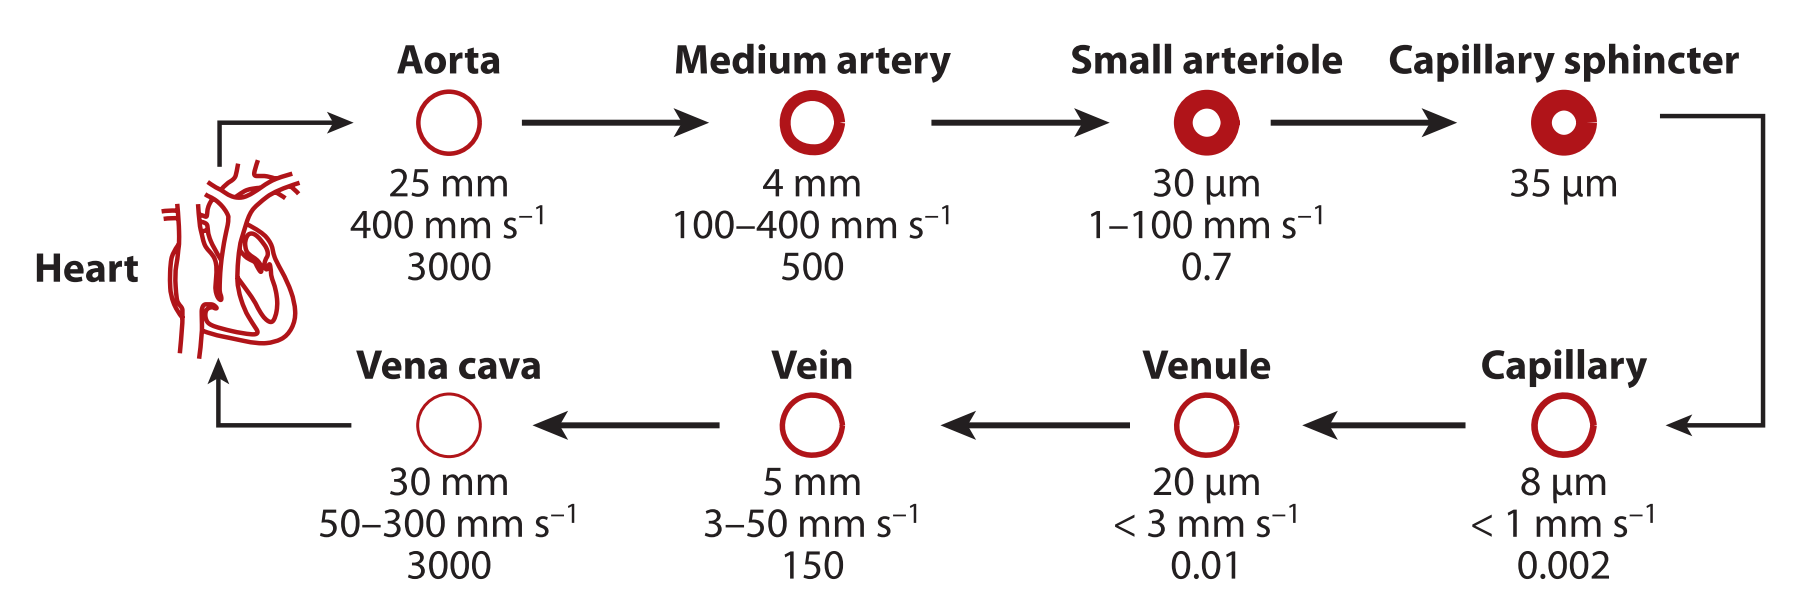
\includegraphics[width=1\textwidth]{Pictures/Bloodvessels.png}
%	\caption{Vessels of the cardiovascular systems and their properties: inner diameter, average blood-flow velocity, and Reynolds number from \cite{berger1996}}
%	\label{fig:veins}
%\end{figure}


\section{High Fields}

Mathematically this will be the easier case to solve. By assuming a very high applied field $\textbf{H}_\text{app}$ the ferromagnetic material will saturate, such that the magnetization becomes uniform:

\begin{equation}
\textbf{M}(\textbf{r}) = \textbf{M}_s \quad \forall \textbf{r}
\end{equation}

where $\textbf{M}_s$ points in the direction of the applied field and has magnitude $M_s$ which is the saturation magnetization of the material.

\begin{equation}
\textbf{M}_s = \frac{\textbf{H}_\text{app}}{|\textbf{H}_\text{app}|}M_s 
\end{equation}

\subsection{The Demagnetization Tensor}

We will now analyze how the demagnetization field looks like. We apply the high-fields case in its definition and we simplify:

\begin{equation}
\textbf{H}_d(\textbf{r}) = - \mathcal{N}(\textbf{r},\textbf{M}) = - \mathcal{N}(\textbf{r},\textbf{M}_s) = - \underbrace{\mathcal{N}(\textbf{r},I)}_{N(\textbf{r}):=}\textbf{M}_s
\end{equation}

Since we can take out the magnetization out of the integral operator we can define a tensor (by evaluating the integral over the identity matrix) that is only shape dependent. We will call this tensor, the demagnetization tensor. We can now write:


\begin{equation}
\textbf{H}_d(\textbf{r}) = -N(\textbf{r})\textbf{M}_s
\end{equation}

Which means that the total H-field is:

\begin{equation}
\textbf{H}(\textbf{r}) = -N(\textbf{r})\textbf{M}_s  + \textbf{H}_\text{app}
\end{equation}

\subsection{Analytical Calculation}

To calculate the demagnetization factor $N(\textbf{r})$ analytically, we only have to evaluate the integral operator defined above over the identity matrix:

\begin{equation}
N(\textbf{r}) := \mathcal{N}(\textbf{r},I) = \frac{1}{4\pi}\oint\limits_{\partial V}  \frac{(\textbf{r}'-\textbf{r})}{|\textbf{r}'-\textbf{r}|^3}\textbf{n}^T\;\mathrm{d}^2r'
\end{equation}


\subsection{Calculation over Simulation}

When performing a simulation with COMSOL, we set the material parameters as well as the shape of our bodies and subject them to the applied field. As an output, we get the H-Field as well as the magnetization in every point in the space. In the Appendix one can find the details to the simulation parameters used in COMSOL.\\

To calculate the demagnetization factor through the simulation, we use our integral equation and create three sets of linearly independent equations for three different linearly independent applied fields. Such that:

\begin{equation}
H(\textbf{r}) = -N(\textbf{r})M(\textbf{r}) + H_\text{app}
\end{equation}

where:

\begin{subequations}
\begin{equation}
H(\textbf{r}) := [\textbf{H}_1(\textbf{r}), \textbf{H}_2(\textbf{r}), \textbf{H}_3(\textbf{r})]
\end{equation}
\begin{equation}
M(\textbf{r}) := [\textbf{M}_1(\textbf{r}), \textbf{M}_2(\textbf{r}), \textbf{M}_3(\textbf{r})]
\end{equation}
\begin{equation}
H_\text{app} := [\textbf{H}_{\text{app},1}, \textbf{H}_{\text{app},2}, \textbf{H}_{\text{app},3}
\end{equation}
\end{subequations}

We solve to the demagnetization tensor and become:

\begin{equation}
N(\textbf{r}) = ( H_\text{app}-H(\textbf{r}) )M^{-1}
\end{equation}

If we're working with "high enough" applied fields, the magnetization will be approximately saturated. Since the applied fields are linearly independent the magnetization vectors will point in the direction of the correspondent applied fields, and thus will also be linearly independent, which makes the tensor $M$ nonsingular, such that its inverse always exists.\\

The problem with the method above, is that, depending on the shape, some directions at certain points in the body are more difficult to saturate. In other words they need much higher fields to achieve its saturation magnetization. However, COMSOL allows us to define a certain predefined, permanent magnetization for our helices. This is convenient to us, because we can avoid the step of adding an applied field by just forcing a certain constant magnetization over the whole body and using the relation between the magnetization and the demagnetization field it generates. Since a constant magnetization can only achieved through saturation, we can simulate a saturated body through setting a uniform magnetization. Similarly to the case above, we calculate the case for three linearly independant magnetizations (thus ensuring non-singularity on the demagnetization matrix) and calculate the demagnetization factor through the following relation:

\begin{equation}
H(\textbf{r}) = H_d(\textbf{r}) =  -N(\textbf{r})M
\end{equation}

The magnitude of the chosen magnetization will be canceled out by the proportional magnitude of the generated H-field. This is consistent with the fact of the demagnetization factor being just a form factor which doesn't depend on any field-related quantity. This is clear by reformulating the equation above:

\begin{equation}
N(\textbf{r}) = -H(\textbf{r})M^{-1}
\end{equation}

\subsubsection{Averaged Values}

Since we're dealing with the overall characteristics of a magnetic body, it makes sense to set the definitions of averaged values clearly. For example, the experimental results obtained through a VSM are of averaged nature. Also, most research papers that deal with demagnetization factors, assign one demagnetization matrix to a certain body (although, as we saw, there is a demagnetization factor for every point in it). It is convenient to use averaged values over the whole body and to be clear what are the characteristics of the its formal definition. In this section we will derive said definitions and its characteristics.\\

We define an averaging operator:

\begin{equation}
\langle \cdot \rangle := \frac{1}{V}\int\limits_V \cdot \;\text{d}^3r
\end{equation}

Where $V$ is the total volume of the body. We can now apply the definition to our integral equation:

\begin{equation}
\langle \textbf{H}(\textbf{r})\rangle = \langle-N(\textbf{r})\textbf{M}_s  + \textbf{H}_\text{app} \rangle
\end{equation}

which, using linearity of the average operator, leads to:

\begin{equation}
\langle \textbf{H}(\textbf{r})\rangle = -\langle N(\textbf{r}) \rangle\textbf{M}_s  + \textbf{H}_\text{app}
\end{equation}

We can use this to derive the calculations out of the simulations by applying the averaging operator on our simulation equations:

\begin{equation}
\langle N(\textbf{r}) \rangle = ( H_\text{app}-\langle H(\textbf{r})\rangle )M^{-1} 
\end{equation}

and

\begin{equation}
\langle N(\textbf{r}) \rangle = -\langle H(\textbf{r})\rangle M^{-1} 
\end{equation}

Which is a very interesting characteristic. It basically shows us that in order to calculate the average demagnetization tensor over the whole volume we simply calculate the average H-field instead of having to calculate the demagnetization tensor in every point and then averaging over the whole volume. \\

From now on, no explicit dependence of location is written next to a variable, matrix or field, we will assume it is an averaged value, e.g.:
\begin{equation}
N := \langle N(\textbf{r}) \rangle
\end{equation}


\subsection{Properties}

From the its definition, it is easy to see that the demagnetization tensor $N(\textbf{r})$ is symmetric and has therefore a set of orthonormal eigenvectors that diagonalize it it\footnote{If a matrix A is symmetric (i.e. $A^T = A$) its eigenvalues are orthogonal. Proof: We have two eigenvectors $\textbf{x}$ and $\textbf{y}$ with their respective eigenvalues $\lambda$ and $\mu$. We then have $A\textbf{x} = \lambda\textbf{x} \Rightarrow \textbf{y}^TA\textbf{x} = \textbf{y}^T \lambda\textbf{x} \Rightarrow (A^T\textbf{y})^T\textbf{x} = \textbf{y}^T \lambda\textbf{x}  \Rightarrow (A\textbf{y})^T\textbf{x} = \textbf{y}^T \lambda\textbf{x}  \Rightarrow \mu\textbf{y}^T\textbf{x} = \textbf{y}^T \lambda\textbf{x} \Rightarrow (\mu - \lambda)\textbf{y}^T\textbf{x} = 0 \Rightarrow \textbf{y}^T\textbf{x} = 0 $ }. \\

Another property proven in \cite{Schlomann1962} is that its trace always sums up to one:

\begin{equation}
\text{trace}(N(\textbf{r})) = 1 \quad \forall \textbf{r} \in V
\end{equation}

 Applying the average operator on both sides of the previous equation and exploiting its linearity as well as the linearity of the trace function we become:

\begin{equation}
\text{trace}(\langle N(\textbf{r})\rangle) = \text{trace}(N)= 1
\end{equation}

In other words, the trace of the averaged demagnetization tensor is also equals to one.\\

Later in the report, we will be able to proof mathematically that for soft-magnetic materials (not necessarily with high magnetic permeability) the demagnetization factor will directly tell us in what direction the body magnetizes the easiest, the so called `''easy axes'' of magnetization. In addition to this, when the body has high permeability, the eigenvalues of the demagnetization factor tell us directly which directions magnetize easier and which harder. Smaller eigenvalues means easier magnetization whereas higher values mean that the correspondent direction is harder to magnetize.

\subsection{Validation}
Our point of reference for every calculation, will always be the simulation with COMSOL. In order to be able to take the correctness of our simulations for granted we need to validate them for shapes where the integral operator can be solved and averaged in a closed form such that an algebraic formula can be used. This is the case for Ellipsoids and Rectangles.

\subsubsection{Rectangles}
The analytical value of the demagnetization matrix $N$ for a rectangular prism is calculated according to \cite{Aharoni1998}. \\

\begin{figure}[ht]
	\centering
  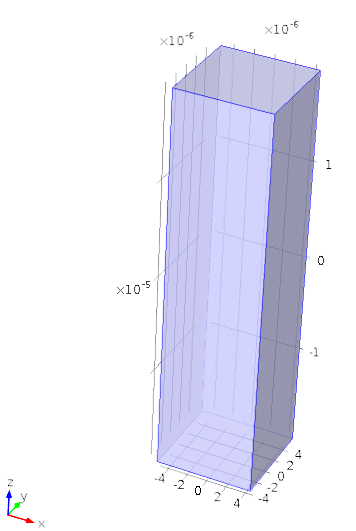
\includegraphics[width=0.4\textwidth]{Pictures/rectangle.png}
	\caption{Magnetic rectangle with displayed dimensions (in meter) for simulation in COMSOL}
	\label{fig:rectangle}
\end{figure}

After having used the formulate shown by \cite{Aharoni1998} and having calculated the (averaged) demagnetization tensors as well as the We compare the numerical calculation with COMSOL (see Figure \ref{fig:rectangle}) with the closed algebraically calculated value and become very little error (see Figure \ref{fig:N_rectangle}). We do the same with the Ellipsoids

\begin{figure}[ht]
	\centering
  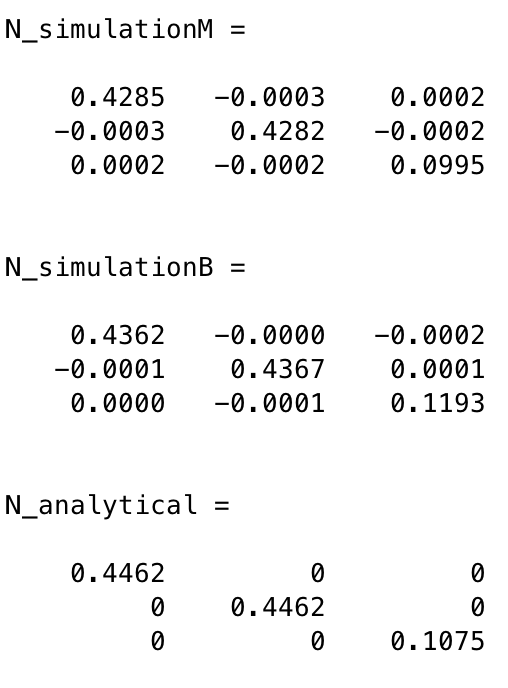
\includegraphics[width=0.4\textwidth]{Pictures/N_rectangle.png}
	\caption{Demagnetization matrices for a magnetic rectangle calculated trough the two explained methods in COMSOL and its analytical value}
	\label{fig:N_rectangle}
\end{figure}

\subsubsection{Ellipsoids}

Ellipsoids will not only help us validate our COMSOL environment, but it is a shape that shows interesting magnetic characteristics. First of all, it always magnetizes uniformly when put inside a uniform applied field. This means that every point in the body will have the same magnetization vector. This will be useful to analyze certain material characteristics when dealing with low applied fields. As a consequence of this, the demagnetization factor doesn't need to be averaged, since it's constant all over the body. \\

The second property is the fact that the demagnetization factor $N$ is a diagonal matrix if displayed in the coordinate system of the ellipsoid semi-axes. This means that the semi-axes of the ellipse are the eigenvalues of the matrix. In other words, an applied field in the direction of one of the ellipsoid axes will magnetize the ellipsoid in that specific direction.\\

\begin{figure}[ht]
	\centering
  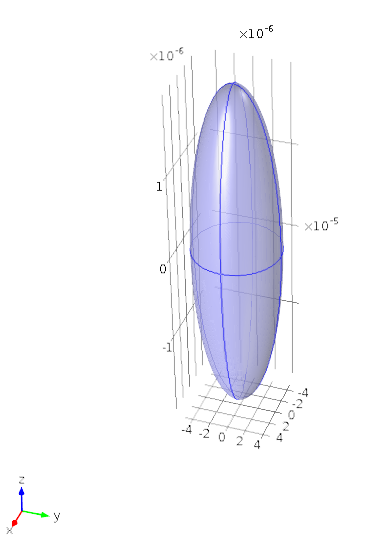
\includegraphics[width=0.4\textwidth]{Pictures/ellipsoid.png}
	\caption{Magnetic ellipsoid with displayed dimensions (in meter) for simulation in COMSOL}
	\label{fig:ellipsoid}
\end{figure}

In Figure \ref{fig:ellipsoid} we see the dimensions of the analyzed ellipsoid and in Figure \ref{fig:N_ellipsoid} the results of the calculations.\\

\begin{figure}[ht]
	\centering
  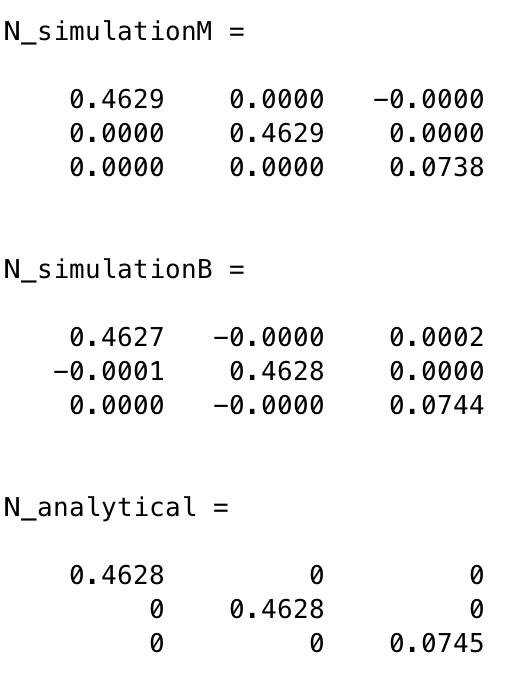
\includegraphics[width=0.4\textwidth]{Pictures/N_ellipsoid.png}
	\caption{Demagnetization matrices for a magnetic ellipsoid calculated trough the two explained methods in COMSOL and its analytical value}
	\label{fig:N_ellipsoid}
\end{figure}

Again, we were able to validate our COMSOL environment since the demagnetization matrices display little error.\\

The second property showed before regarding ellipsoids is used in the literature as a powerful tool to show the magnetization characteristics of other, more complicated magnetic bodies. Since every soft-magnetic body with high permeability will have a demagnetization factor $N$, it will also have easy axes of magnetization, which will be the eigenvalues of the matrix. Since the matrix can be diagonalized in the coordinate system of this easy axes, one can define a so-called ''equivalent ellipsoid'' which will not only have the same volume, but also the same easy axes, as well as the same ratio of the inverse-eigenvalues displayed by its semi-axes.\\

\begin{figure}[ht]
	\centering
  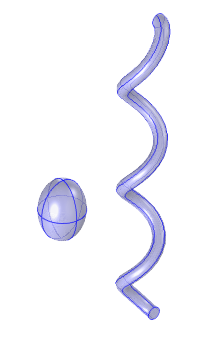
\includegraphics[width=0.25\textwidth]{Pictures/eqell.png}
	\caption{Equivalent ellipsoid of a helical soft-magnetic body with high permeability}
	\label{fig:eqell}
\end{figure}

Figure \ref{fig:eqell} shows the equivalent ellipsoid of a helical body with high permeability. From the direction and length of the body's semi-axes one can directly read that the most elongated  direction of the helix is the direction where it magnetizes the easiest. Whereas the two remaining easy-axes is where it would magnetize the hardest.


\subsection{Helical Bodies}

The real challenge of evaluating the demagnetization factor of our helices is an effective and efficient way of calculating this surface integral numerically. Matlab allows us to evaluate two-dimensional integrals in a straight forward way, but since our surface is curved we have to set up the integral in the appropriate coordinate system. \\


For the helical bodies, as we mentioned before, we assumed a soft-magnetic behavior with high permeability. We analyzed then the helices H1 to H10 being fully magnetic, thin coated and half coated and we compared the two methods exposed above, through numerical approximation of the surface integral as well as simulation.Since the axes of magnetization of the helices are almost aligned with the coordinate system, we will only present the diagonal values of the matrices.\\

\begin{figure}[ht]
	\centering
  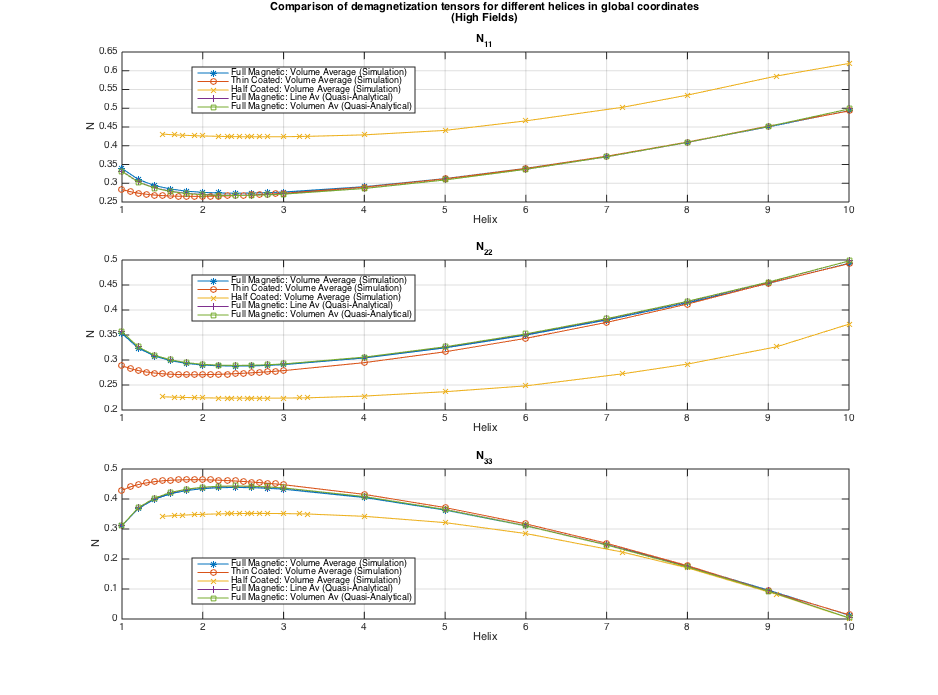
\includegraphics[width=1\textwidth]{Pictures/DemagFactors_Comparison_High.png}
	\caption{Diagonal values of demagnetization matrices of helical soft-magnetic helices with high permeability}
	\label{fig:DemagHigh}
\end{figure}

Figure \ref{fig:DemagHigh} shows said values for the simulations of full magnetic, thin coated and half coated helices against its quasi-analytical counterparts (numerical evaluation of the integral). For the case of half-coated helices, only a simulation was performed, since the mathematical definition of the magnetic volume for one sided thin coating was too complex. Since we are dealing with average values, in the case of the quasi-analytical calculation of the demagnetization factors, only a finite amount of points along the body where evaluated and then averaged. Additionally for the sake of comparison, a line average was done, where only points along the central line of the helix wire were calculated and averaged.\\

One can also see that for the case of the half-coated helices, different elongation indexes were used. The reason for this is the complexity of the meshing process in the simulation that often didn't allowed certain specific shapes. The method used to model the half-coated helices, was by subtracting two full helices which where shifted by a very small distance (200nm which is the coating thickness), thus leaving only a thin shell that resembles a half coated helix (See Figure \ref{fig:halfcoated}). \\

\begin{figure}[ht]
	\centering
  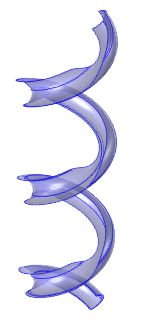
\includegraphics[width=0.2\textwidth]{Pictures/halfcoated.png}
	\caption{3D model of half coated elongated helix}
	\label{fig:halfcoated}
\end{figure}

The problem is that for coiled up elongations like H1, this method doesn't resemble the half-coating anymore and is therefore wrong (See Figure \ref{fig:halfcoatedcoiled}). That is the reason why shapes near H1 were not taken into consideration in the calculations.\\

\begin{figure}[ht]
	\centering
  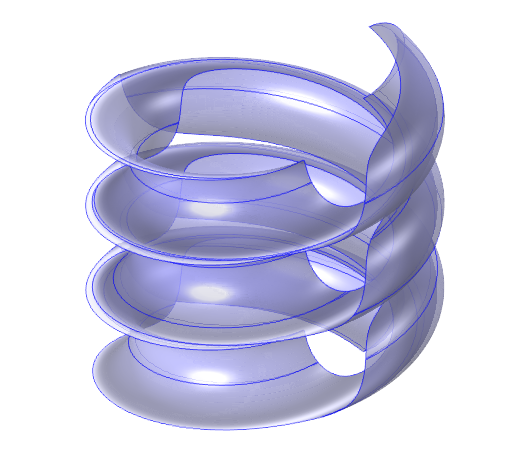
\includegraphics[width=0.2\textwidth]{Pictures/halfcoatedcoiled.png}
	\caption{3D model of half coated coiled-up helix}
	\label{fig:halfcoatedcoiled}
\end{figure}

For high permeabilities, one can calculate the misalignment angle of the helices towards its axes by analyzing the eigenvalues and eigenvectors of the demagnetization factor in the following fashion:

\begin{equation}
\theta = \arccos(\textbf{v}_\text{min})
\end{equation}

where $\textbf{v}_\text{min} $ is the normed eigenvector corresponding to the easy axes that is the easiest to magnetize, in other words, the one corresponding to the smallest eigenvalue of $N$. We plot then the angles and compare them to existing experimental data regarding the misalignment angles.\\

\begin{figure}[ht]
	\centering
  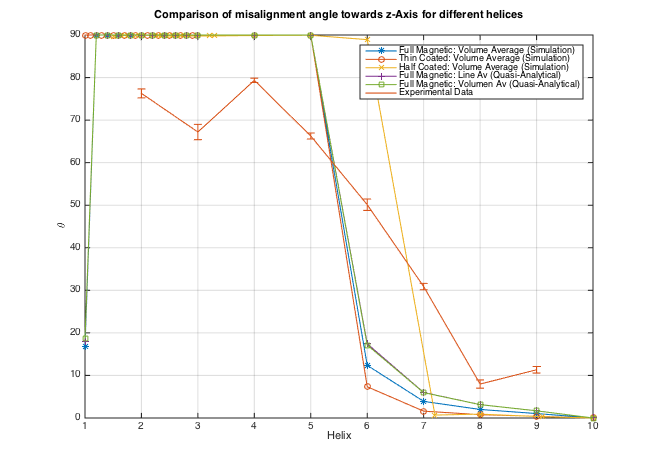
\includegraphics[width=1\textwidth]{Pictures/MisalignmentAngles_high.png}
	\caption{Misalignment angles of helical soft-magnetic helices with high permeability}
	\label{fig:MisalignmentAngles_high}
\end{figure}

FIgures \ref{fig:DemagHigh} and \ref{fig:MisalignmentAngles_high} help us see how accurate the quasi-analytical (numerical) calculation is compared to the simulations for full and thin helical bodies. We also see that the trend of the misalignment angle of the experimental results is captured by the simulations and quasi-analytical calculations.


\begin{figure}[ht]
	\centering
  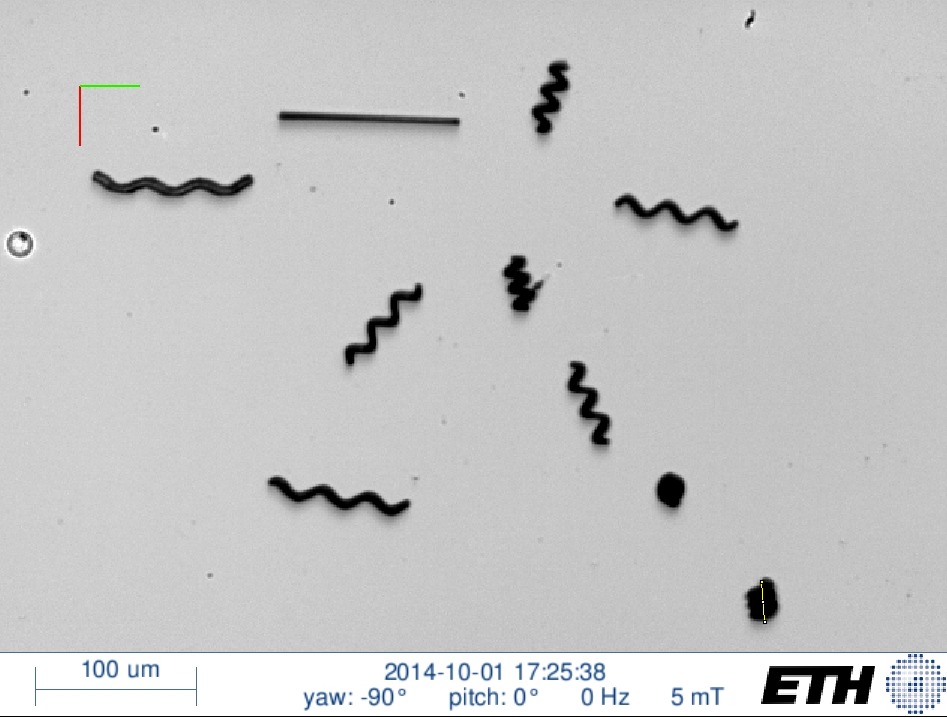
\includegraphics[width=0.8\textwidth]{Pictures/MisalignmentExperimental.png}
	\caption{Misalignment angles of helical soft-magnetic helices (experimental data)}
	\label{fig:MisalignmentExperimental}
\end{figure}



\newpage\mbox{}\newpage
%!TEX root = thesis.tex
\section{Low Fields}

Similar to the previous chapter, we will start this one by defining what is meant by low applied magnetic fields. As we saw before, we are dealing with polycrystalline ferromagnetic bodies which, in general, are highly non-linear and they show a hysteretical behavior. In order to analyze the case of low fields in a meaningful way that, in addition behaves less complex mathematically, we took first the assumption of our material being soft magnetic, taking away the hysteretic behavior. The next step, will be to tackle the nonlinearity by analyzing the two different cases: high fields and low fields. In both of these cases, we linearize our curve. In the high fields case to be a constant (saturation) and in this case to be a linear relation of the following structure.

\begin{equation}
\textbf{M}(\textbf{r}) = \chi_m \textbf{H}(\textbf{r})
\end{equation}

Although we already used this variable name to describe the nonlinear curve we will be consistent with the convention of using for low fields $\chi_m$ as a constant parameter. 

\subsection{The Demagnetization Tensor}

Now that there is a relation that tells us how the body magnetizes for low fields, we can combine it to our integral equation (that basically calculates how the magnetic field looks like for a magnetized body). The solution to the equation is the real physical state that our body achieves.

\begin{equation}
\frac{1}{\chi_m}\textbf{M}(\textbf{r}) = -\mathcal{N}(\textbf{r},\textbf{M}(\textbf{r}))  + \textbf{H}_\text{app}
\end{equation}

Since there's a linear relation between the total H-Field and the magnetization we can either solve the above equation to $\textbf{M}$ or to $\textbf{H}$. In our case it will be convenient to solve it to $\textbf{M}$.\\

Although there is no general closed solution to the above equation, it can be proved (see Appendix \ref{s:LinearityIntegralEquation}) that the magnetization $\textbf{M}(\textbf{r})$ is linear towards the the applied field $\textbf{H}_\text{app}$. From that it follows that the demagnetization field  $\textbf{H}_d(\textbf{r})$ and the total H-Field $\textbf{H}(\textbf{r})$ also are. The main theorems of linear algebra allow us to describe any linear relation through a matrix multiplication. We can therefore define a new matrix $\Psi(\textbf{r})$:

\begin{equation}
\textbf{M}(\textbf{r}) = \Psi(\textbf{r})\textbf{H}_\text{app}
\end{equation}

from the definition of the demagnetization field it follows:

\begin{equation}
\textbf{H}_d(\textbf{r}) = \left(\frac{1}{\chi_m}\Psi(\textbf{r})-I\right)\textbf{H}_\text{app}
\end{equation}

and the total field:

\begin{equation}
\textbf{H}(\textbf{r}) = \frac{1}{\chi_m}\Psi(\textbf{r})\textbf{H}_\text{app}
\end{equation}

Our integral equation now becomes:

\begin{equation}
\frac{1}{\chi_m}\Psi(\textbf{r}) = -\mathcal{N}(\textbf{r},\Psi(\textbf{r}))  + I
\end{equation}

and its solution, the matrix function $\Psi(\textbf{r})$.\\

The problem here, is that we have no clear definition of what the demagnetization factor for low fields may be. We define it then, to be consistent to the high fields case: We use the a set of three linearly independent applied fields and construct the matrices $H_\text{app}$, $M(\textbf{r})$, $H(\textbf{r})$ and $H_d(\textbf{r})$ such that:

\begin{subequations}
\begin{equation}
H(\textbf{r}) := [\textbf{H}_1(\textbf{r}), \textbf{H}_2(\textbf{r}), \textbf{H}_3(\textbf{r})]
\end{equation}
\begin{equation}
M(\textbf{r}) := [\textbf{M}_1(\textbf{r}), \textbf{M}_2(\textbf{r}), \textbf{M}_3(\textbf{r})]
\end{equation}
\begin{equation}
H_\text{app} := [\textbf{H}_{\text{app},1}, \textbf{H}_{\text{app},2}, \textbf{H}_{\text{app},3}]
\end{equation}
\end{subequations}

We now define the demagnetization tensor for low fields in the following way:

\begin{equation}
N(\textbf{r}) := -H_d(\textbf{r})\,M(\textbf{r})^{-1}
\end{equation}

and through simplification we get\footnote{a detailed derivation can be found in Appendix \ref{s:DemagPsi}}:

\begin{equation}
N(\textbf{r}) = \Psi(\textbf{r})^{-1} - \frac{1}{\chi_m}I
\end{equation}

\subsection{Calculation through simulation}

Like in the case of high fields, our basic calculation will be the simulation in COMSOL. For this part, the same models, meshes and assumptions were used, with the difference that here, a linear model was used instead of a non-linear one that can be saturated. The reason for this is to be consistent with the fact that we are dealing with low fields, which makes the model act linearly. \\

We will use the same method as before calculating the magnetization for three linear independent applied fields and calculating the demagnetization factor with the following relation:

\begin{equation}
 N(\textbf{r}) =  H_d(\textbf{r})   M(\textbf{r})  ^{-1}
\end{equation}

which is correct and consistent to our definition for low fields.

\subsubsection{Averaged Values}

Since, again, we are dealing with averaged values, it is very important to leave clear mathematically what we are doing while taking any assumption. In the case of high fields (saturated case), the magnetization of the body is assumed to be constant. One could write it in the following fashion:

\begin{equation}
\langle N(\textbf{r}) \rangle = \langle H_d(\textbf{r}) \rangle  M_s ^{-1} = \langle H_d(\textbf{r}) \rangle \langle M(\textbf{r}) \rangle ^{-1}
\end{equation}

This basically says, that the averaged demagnetization matrix can be calculated as a product of two averaged matrices. Since the magnetization matrix is anyways constant, averaging has no effect on it. However in the low field case, the averaged demagnetization tensor is not the product of the averaged applied field matrix and the inverse of the averaged magnetization matrix. Since

\begin{equation}
\langle N(\textbf{r}) \rangle = \langle \Psi({\textbf{r})}^{-1}\rangle - \frac{1}{\chi_m}I
\end{equation}

and

\begin{equation}
 \langle H_d(\textbf{r}) \rangle \langle M(\textbf{r}) \rangle ^{-1} = \langle \Psi({\textbf{r})}\rangle^{-1} - \frac{1}{\chi_m}I
\end{equation}

However, we will make the assumption of $\langle\Psi(\textbf{r})\rangle^{-1} \approx \langle\Psi(\textbf{r})^{-1}\rangle$ in order to perform our calculations over simulations in the same fashion as it has been explained before, thus using the following relation:

\begin{equation}
\langle N(\textbf{r}) \rangle \approx \langle H_d(\textbf{r}) \rangle \langle M(\textbf{r}) \rangle ^{-1}
\end{equation}

An deep analysis and further research on this topic will be need in order to assess the correctness of this assumption. The mathematical properties of the demagnetization matrix depending on the properties of $\Psi(\textbf{r})$ and $\langle\Psi(\textbf{r})\rangle$ will.

\subsubsection{Results}

Analogously to the high field case, the results of the simulations for the full magnetic, thin coated and half coated are presented in Figure \ref{fig:DemagLow}. 

\begin{figure}[ht]
	\centering
  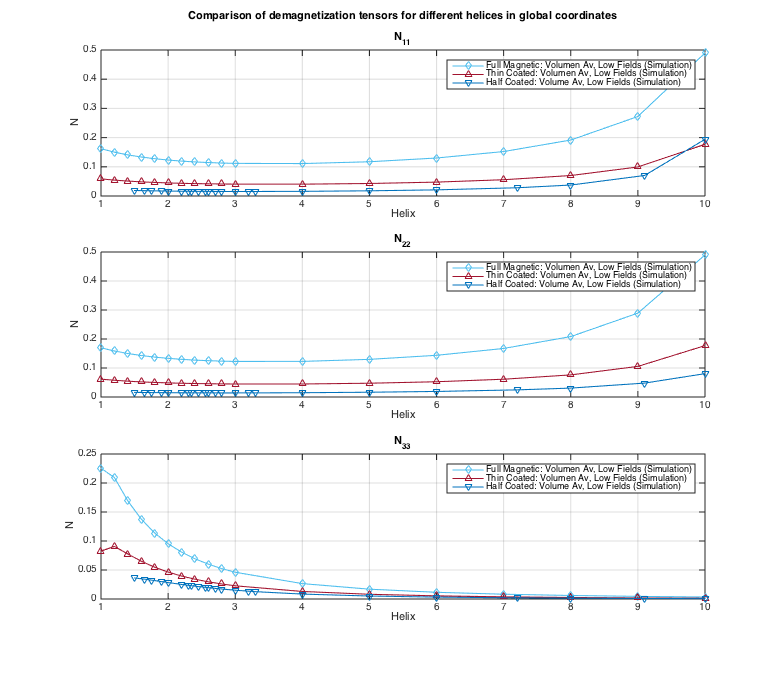
\includegraphics[width=1\textwidth]{Pictures/DemagFactors_Comparison_Low.png}
	\caption{Diagonal values of demagnetization matrices of helical soft-magnetic helices with high permeability at low fields}
	\label{fig:DemagLow}
\end{figure}

The misalignment angles are, again, shown in Figure \ref{fig:MisalignmentAngles_Low} compared to the experimental data.

\begin{figure}[ht]
	\centering
  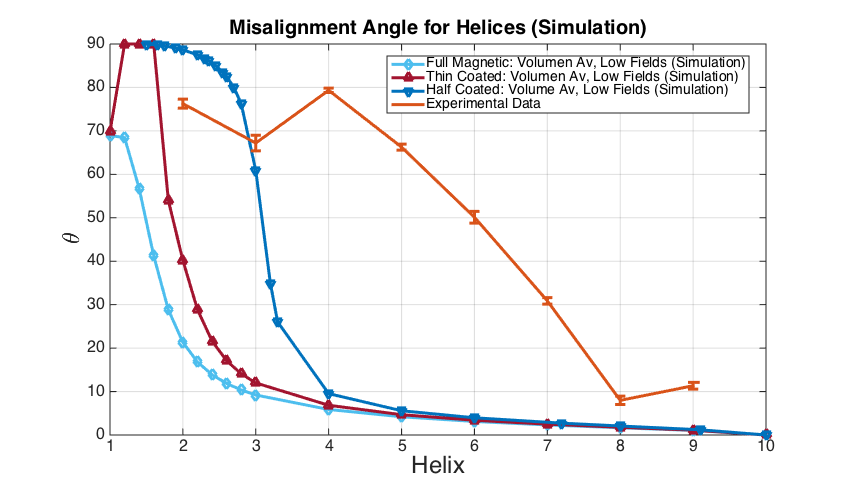
\includegraphics[width=1\textwidth]{Pictures/MisalignmentAngles_Low.png}
	\caption{Misalignment angles of helical soft-magnetic helices with high permeability at low fields}
	\label{fig:MisalignmentAngles_Low}
\end{figure}

In Figure \ref{fig:DemagLow} we clearly see the the same trends on all curves. As expected we a see a very similar behavior between both radial axes (directions 1 and 2), on all three curves. The reason for this is the small influence of the top and bottom end of each helix (it is not an infinitely long helix) which accounts for the differences. 
The results are easier to interpret with the fact that the magnetization of a helix for low fields follows in each point the shape and direction of the helix (See Figure \ref{fig:MagnetLow}\\

In directions 1 and 2 (radial directions) we see that the curves start at a certain level, diminish and then grow again. This means in other words, that the helices magnetize harder for lower helix index in radial direction, then easier and finally hard again. As it was mentioned before, the magnetization points along the shape of the helix. Since the helix is coiled, and we're dealing with the total magnetization, the coiling creates a cancellation of magnetization for most of the helix. When the helix has a more elongated form (not fully elongated) this cancellation effect goes away and the helix magnetizes therefore easier along the specific direction. When the helix is very elongated the helix is almost aligned with the third axes. Since the helix is very slim, it is very difficult to magnetize in radial directions.\\

In the case of direction 3 we see a constant drop from the coiled helices to the more elongated helices. The reason for this is that, when the helix is coiled, it is hard to magnetize in the third direction, which is the direction perpendicular to the helix's shape line. When the helix elongates, the helix's shape line aligns more and more with the third direction, which makes every time more easy to magnetize, the more the helix elongates, therefore the drop in the demagnetization factor.\\

The discrepancies between the three types of helix fillings (full, thin shell and half-coated) is due to the fact that the body magnetizes easier along the thin film. In the case of thin shell, the helix magnetizes easier along the wall, but the fact of it being round accounts also for cancellations in the field (depending on the direction of the applied field). In the case of the half-coated helices, the cancellation doesn't appear. The coiling of the helix but also the local orientation combined with the type of filling create complex interactions, which account for the shifting of the curves. The plots are evidence, that the coiling of the helix is the predominant factor when it comes to the qualitative, main magnetic behavior of the helix, and not the type of filling of it. \\

Figure \ref{fig:MisalignmentAngles_Low} we see the misalignment angles compared to the experimentally measured misalignment angles. Again, we captured the trend of the misalignment angle: For low coiled helices, the misalignment angle tends towards a perpendicular alignment with the applied field, whereas, as expected, for more elongated helices the alignment correspond to the direction of the applied field, behaving more like a compass needle.\\

\begin{figure}[ht]
	\centering
  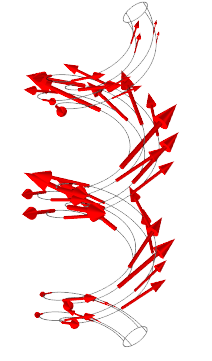
\includegraphics[width=0.2\textwidth]{Pictures/MagnetLow.png}
	\caption{Graphical representation of magnetization of a ferromagnetic helix in low fields. The arrows (red) represent the magnetization vectors in different points along the helix}
	\label{fig:MagnetLow}
\end{figure}


\subsection{Analytical Calculation}

Contrary to the high field case, where the demagnetization factor is only a surface integral matrix, for the low field case, one has to solve the surface integral matrix equation:

\begin{equation}
\frac{1}{\chi_m}\Psi(\textbf{r}) = -\mathcal{N}(\textbf{r},\Psi(\textbf{r}))  + I
\end{equation}

the demagnetization factor is then:

\begin{equation}
N(\textbf{r}) = \Psi(\textbf{r})^{-1} - \frac{1}{\chi_m}I
\end{equation}

From the problem formulation, the solution seems to be uncomplicated. However this was one of the biggest challenges throughout this report. The first approach was to approximate our integral equation by a line integral, by assuming that the integrand doesn't change much from the center to the edges (since the wire is very thin).This turned our surface integral equation into a so called Fredholm integral equation with a linear integral operator in it (see Appendix) for which there exist literature that tackles the problem of solving it numerically (see  \cite{Allahviranloo2011}, \cite{Babolian2004}, \cite{DeBonis2008}, \cite{Hameed2011}, \cite{Jafarian2012}, \cite{Karimi2015}, \cite{Maleknejad2005},\cite{Rashidinia2007}, \cite{Ray2013}, \cite{Saeed2008}). After unsuccessful implementation of various methods (mainly because of the numerical complexity) we developed the following algorithm to solve it.

\subsubsection{Solving Algorithm}

In this subsection we'll explain the numerical algorithm used to solve the Matrix integral equation shown above. The principle lies in the idea of approximating each component of the matrix $\Psi(s)$ by another function. The choice of these approximations were Fourier series and Legendre polynomials.\\

Lets write our matrix $\Psi(s)$ as an approximation $\hat{\Psi}(s)$ of some basic functions. For the component $i,j$ we have:

\begin{subequations}
\begin{equation}
\hat{\Psi}_{i,j}(s)  = c_{i,j}^1f_1(s) + c_{i,j}^Nf_N(s) + ... + c_{i,j}^Nf_N(s) = 
\end{equation}
\begin{equation}
\underbrace{ \left[ 
\begin{array} {c}
c_{i,j}^1 \\
c_{i,j}^2 \\
\vdots \\
c_{i,j}^N \\
\end{array}\right]}_{=:c_{i,j}} \cdot \underbrace{\left[ 
\begin{array} {c}
f_1(s) \\
f_2(s) \\
\vdots \\
f_N(s) \\
\end{array}\right]}_{=:f(s)}
\end{equation}
\end{subequations}

We can then write the matrix in the following way:

\begin{equation}
\hat{\Psi}(s) = \underbrace{ \left(\begin{array}{ccc}
f(s)^T & 0 \dots &  \dots 0 \\
0 \dots & f(s)^T & \dots 0 \\
0 \dots & \dots 0 & f(s)^T\\
\end{array} \right)}_{=:F(s)}\underbrace{ \left(\begin{array}{ccc}
c_{1,1} & c_{1,2} & c_{1,3}   \\
c_{2,1} & c_{2,2} & c_{2,3}   \\
c_{3,1} & c_{3,2} & c_{3,3}   \\
\end{array} \right)}_{=:C}
\end{equation}

If we plug our approximation in the integral equation we get:
\begin{subequations}
\begin{equation}
\frac{1}{\chi_m}\hat{\Psi}(s) = - \mathcal{N}(\hat{\Psi}(s)) + I
\end{equation}
\begin{equation}
\frac{1}{\chi_m}F(s)C = - \mathcal{N}(F(s))C + I
\end{equation}
\begin{equation}
\frac{1}{\chi_m}(F(s) + \mathcal{N}(F(s)))C  = I
\end{equation}
\begin{equation}
(F(s) + \mathcal{N}(F(s)))C  = \chi_mI
\end{equation}
\end{subequations}

The matrix $(F(s) + \mathcal{N}(F(s)))$ is a $3\times 3N$ Matrix. So in order to make it square we evaluate it at $N$ points of $s$. We become then:


\begin{equation}
\underbrace{\left[ \begin{array}{c}
(F(s_1) + \mathcal{N}(F(s_1)))   \\
(F(s_2) + \mathcal{N}(F(s_2)))  \\
\vdots \\
(F(s_N) + \mathcal{N}(F(s_3)))  \\
\end{array} \right]}_{:=A} C = 
\underbrace{\left[ \begin{array}{c}
\chi_mI  \\
\chi_mI  \\
\vdots \\
\chi_mI  \\
\end{array} \right]}_{:=B}
\end{equation}

And finally:

\begin{equation}
C = A^{-1}B
\end{equation}


This means that we reduced our integral equation to a linear system, where we have to calculate $9N^2$ integrals.\\

Unfortunately the results obtained by this algorithm were not successful (mainly due to no convergence and singularities in the results) and the task of solving the integral equation was left for further research. \\

The methods of solving problems in magnetostatics is a topic that has been researched for many decades. We will leave further research try to approach the problem using the methods used until now. For more information, refer to:\cite{Babic2000}, \cite{Canova2001}, \cite{Hafla2005}, \cite{Hafla2006a}, \cite{Hafla2006}, \cite{Hafla2006b}, \cite{Han1994}, \cite{Le-van2015}, \cite{Maleknejad2005}, \cite{Nicolazzi2005}, \cite{Nicolet1994}, \cite{Sertel2002}, \cite{Shahi2009} and \cite{VandeWiele2008}.

\newpage\mbox{}\newpage
%!TEX root = thesis.tex

\section{Experimental Assesment}

In order to be able to validate our theoretical results done in the previous parts, we used the help of a VSM setup to measure the magnetization of real macro-helices and calculate with it their demagnetization matrices. On parallel, the same macrohelices were modelled in COMSOL in order for the theoretical demagnetization matrix to be calculated.\\

\begin{figure}[ht]
	\centering
  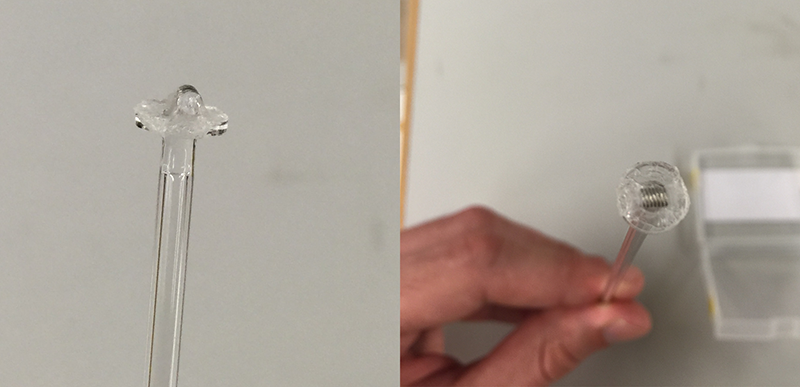
\includegraphics[width=0.8\textwidth]{Pictures/Macrohelix7.png}
	\caption{Handwired nickel macrohelix ($k=7$)}
	\label{fig:Macrohelix7}
\end{figure}

In Figure \ref{fig:Macrohelix7} we get an insight of the size of the helices we used. The helix was made of pure polycristalline nickel with a width of $d = 250$nm which was coiled around a non-magnetic M2.5 polymer screw and then attached to the measuring VSM probe using non-magnetic glue. The probe was then placed in the VSM setup (Figure \ref{fig:VSMSetup}). Through the shortening of the helix, we were able to do measurements for different number of coilings $k = 2, 3, 4$ and $7$.\\

\begin{figure}[ht]
	\centering
  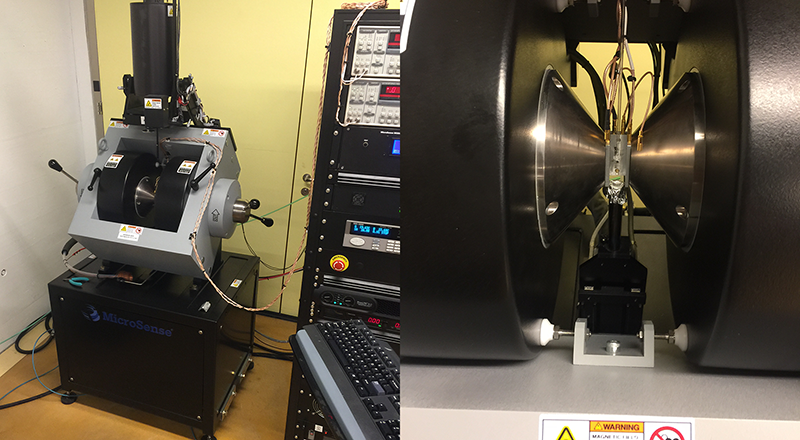
\includegraphics[width=0.8\textwidth]{Pictures/VSMSetup.png}
	\caption{VSM Setup for macrohelix measurements}
	\label{fig:VSMSetup}
\end{figure}

The VSM creates an approximately constant applied magnetic field in one direction to the probe and measures the magnetic moment in the direction of the applied field and the perpendicular direction on the plane parallel to the floor. 
We assumed  that both perpendicular radial directions of the helices are equal, such that we only have to measure one. With the VSM we measured one radial and the axial directions. We create a sweep that increases the applied field from zero to a point where the moment is practically saturated and then reduces it until it saturates in the opposite direction. Then it goes back to the saturate it in the original direction, thus completing the hysteresis loop.\\

\begin{figure}[ht]
	\centering
  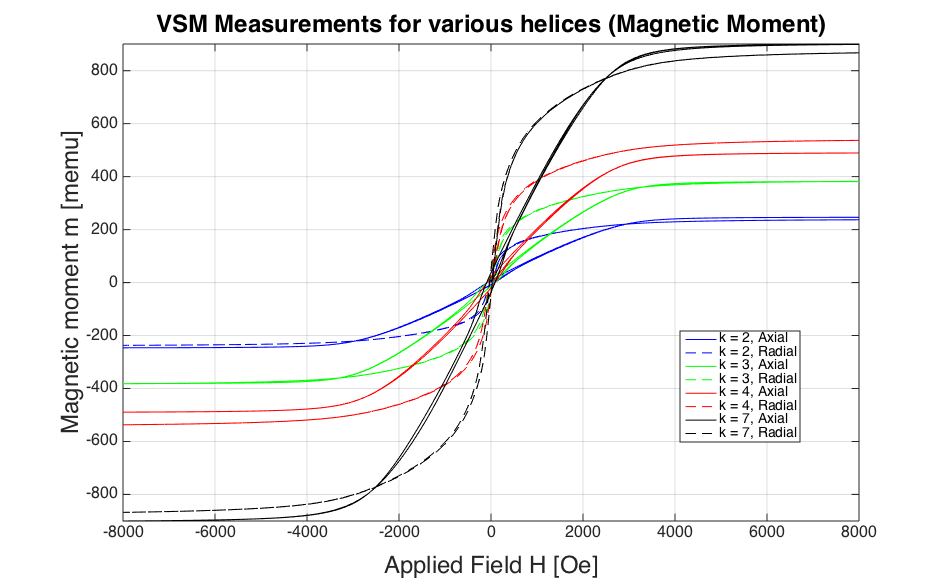
\includegraphics[width=1\textwidth]{Pictures/VSM_Moment.png}
	\caption{Magnetic moment vs. applied field for various coiling numbers $k$}
	\label{fig:VSM_Moment}
\end{figure}

For each the axial applied field and the radial applied field we extract two curves, one in axial and one in radial direction. We have thus four hysteresis loops per helix. An important step before continuing is to make sure that the curves all saturate at the appropiate moment. We calibrate, thus, using the, already given for nickel, mass specific saturation moment:

\begin{equation}
m_s = 54.97 \frac{\text{emu}}{g}
\end{equation}

We will take our integral equation for an applied field in both radial and in axial direction. Since we're dealing with low fields, we will take the linearization of $\chi_m(\textbf{H})$ for small $|\textbf{H}|$. 

%PROOF THAT MISSING VALUES DISSAPPEAR WHEN CALCULATING MISSALIGNMENT ANGLE

\begin{equation}
\frac{1}{\chi_m}\textbf{M}(\textbf{r}) = -N(\textbf{r})\textbf{M}(\textbf{r})  + \textbf{H}_\text{app}
\end{equation}

and we average it:

\begin{equation}
\frac{1}{\chi_m}\langle\textbf{M}(\textbf{r})\rangle = -\langle N(\textbf{r})\textbf{M}(\textbf{r})\rangle  + \textbf{H}_\text{app}
\end{equation}

this relation can be written in the following way\footnote{This is of course an assumption and it should be examined further in detailed to assess the correcness of it. See Appendix \ref{s:NMComparison} for a detailed comparison of both the exact case and the approximation}:

\begin{equation}
\frac{1}{\chi_m}\langle\textbf{M}(\textbf{r})\rangle \approx -\langle N(\textbf{r})\rangle\langle\textbf{M}(\textbf{r})\rangle  + \textbf{H}_\text{app}
\end{equation}
 We insert the relation between the total magnetic moment and the averaged magnetization:

\begin{equation}
\langle{M}(\textbf{r})\rangle = \frac{\textbf{m}}{V}
\end{equation}

We will write now $N$ for $\langle N(\textbf{r})\rangle$

\begin{equation}
\frac{1}{\chi_m}\frac{\textbf{m}}{V} = - N\frac{\textbf{m}}{V}  + \textbf{H}_\text{app}
\end{equation}

we construct our matrix with the axial and both radial applied fields and the correspondant measured magnetic dipoles:

\begin{equation}
\frac{1}{\chi_m}\frac{\textbf{1}}{V}m = - \frac{\textbf{1}}{V}N m  + H_\text{app}
\end{equation}

and we solve to $N$:

\begin{equation}
\frac{\textbf{1}}{V}\frac{1}{\chi_m}m = - \frac{\textbf{1}}{V}N m  + H_\text{app}
\end{equation}

\begin{equation}
N = V\; H_\text{app}\; m^{-1} - \frac{1}{\chi_m}I
\end{equation}

The important part here is that the measurements we do are only in the axial and one radial direction. Therefore we have to fill the missing parts of the matrices $m$ and $H_\text{app}$ with the assumption that both radial directions behave equally\\

In our case, we define $H_\text{app}$ defined in the following way:
\begin{equation}
H_\text{app} = [\textbf{H}_\text{ax}, \textbf{H}_\text{rad,1}, \textbf{H}_\text{rad,2}]
\end{equation}

Where:
\begin{equation}
H_\text{rad,2} =\frac{ \textbf{H}_\text{ax} \times \textbf{H}_\text{rad,1} }{|\textbf{H}_\text{ax} \times \textbf{H}_\text{rad,1}|}\;|\textbf{H}_\text{rad,1}|
\end{equation}

we then have the magnetization matrix obtained from the measurements:

\begin{equation}
m = [\textbf{m}_\text{ax},\textbf{m}_\text{rad,1},\textbf{m}_\text{rad,2}] = \left[\begin{array}{ccc}
m_\text{ax;ax} & m_\text{rad,1;ax} & m_\text{rad,2;ax} \\
m_\text{ax;rad,1} & m_\text{rad,1;rad,1} & m_\text{rad,2;rad,1}\\
m_\text{ax;rad,2} & m_\text{rad,1;rad,2} & m_\text{rad,2;rad,2}
\end{array}\right]
\end{equation}

where $m_\text{ax;ax}$,   $m_\text{rad,1;ax}$, $m_\text{ax;rad,1}$ and $m_\text{rad,1;rad,1}$ are known from the measurements. By assuming symmetry we assume the following for the rest of the values:

\begin{subequations}
\begin{equation}
m_\text{rad,2;ax} = m_\text{rad,1;ax} 
\end{equation}
\begin{equation}
m_\text{ax;rad,2} = m_\text{ax;rad,1} 
\end{equation}
\begin{equation}
 m_\text{rad,2;rad,2} = m_\text{rad,1;rad,1}
\end{equation}
\begin{equation}
m_\text{rad,1;rad,2} = m_\text{rad,2;rad,1} = 0
\end{equation}
\end{subequations}

The latter says that the magnetization in one radial direction when the applied field is in the other radial direction is zero. Altough locally it may not be zero, the symmetry of the helix as well as it having full coilings leads to a cancelling out in this direction \\

\subsection{The Apparent Susceptibility}

Although the whole theory to magnetism was already discussed in previous chapters, we find ourselves in the experimental area. As we saw before, a popular way of measuring magnetization is through a VSM, where the measurable variables are the applied field and the created magnetic torque.\\

Although the demagnetization matrix is the missing, body-dependant variable that completes the unique relation between an applied field and its magnetization, we will find a more direct and experimentally meaningful way of describing this relationship. For this, we start by showing our integral averaged equation for low fields, which simplifies to an algebraic equation (since the demagnetization factor is a constant matrix)\footnote{We will replace the '$\approx$' by '$=$' for simplification purposes as well as $N : = \langle N(\textbf{r})\rangle$ and $\textbf{M} : = \langle \textbf{M}(\textbf{r})\rangle$}:

\begin{equation}
\frac{1}{\chi_m}\textbf{M} =  -N\textbf{M}  + \textbf{H}_\text{app}
\end{equation}

we manipulate the equation ang get:
\begin{equation}
\left(\frac{1}{\chi_m}I+N\right) \textbf{M} = \textbf{H}_\text{app}
\end{equation}

and finally:
\begin{equation}
 \textbf{M} = \underbrace{\left(\frac{1}{\chi_m}I+N\right)^{-1}}_{:= \chi_a}\textbf{H}_\text{app}
\end{equation}

We see a constant, linear mapping between the applied field and the magnetization. We call this constant $\chi_a$, the apparent suceptibility, making an analogy to the structure of the magnetization within a body, which actually happens in each material point within the body with the magnetic suceptibility $\chi_m$:

\begin{equation}
 \textbf{M}(\textbf{r}) = \chi_m\textbf{H}(\textbf{r})
\end{equation}

Although this equation may make more sence from a physical point of view, it is impossible to use it directly to measure the magnetization of a body. We thus use, as mentioned before, the following\footnote{May the reader be aware of the fact that the magnetic susceptibility $\chi_m$, as it was mentioned before, is not only a function of the H-field and is in general a matrix. In this case we are dealing with the linearized version (constant) which can be written as a scalar instead of a diagonal matrix with identical diagonal values due to the crystal anisotropy}:

\begin{equation}
 \textbf{M} = \chi_a\textbf{H}_\text{app}
\end{equation}

\subsubsection{Comparison with the demagnetization matrix N}

From the above calculations we see the relation between the demagnetization matrix and the apparent susceptibility:

\begin{equation}\label{eq:chia}
\chi_a = \left(\frac{1}{\chi_m}I+N\right)^{-1}
\end{equation}

If we analyze the characteristics of both matrices we find two important characteristics:

The first one is that for highly magnetizable bodies, where the intrinsic magnetic susceptibility is high ($\chi_m >>1$) the following holds:

\begin{equation}
\chi_a \approx  N^{-1}
\end{equation}

The second, even more interesting one, is that both $\chi_a$ and $N$ (disregarding of the magnitude of $\chi_m$) share eigenvalues \footnote{See Appendix \ref{s:SameEigen} for proof} and therefore easy axes too. This means also, that we can analyze directly the easy axes of the demagnetization tensor $N_\text{av}$ to see how an applied field will magnetize the whole body. If the body has, in addition, a high magnetic susceptibility, i.e., $\chi_a \approx  N^{-1}$, then the eigenvalues are inverted.\\

If the demagnetization matrix and the apparent susceptibility share eigenvectors and have inverted eigenvalues (for the same eigenvector) means that the demagneti†zation factor has all the information about how the body will align and which directions will magnetize easier. This is the reason why, until now, we could always see out of the demagnetization matrix, which axes magnetize easier.\\

This gives us also a very important practical consequence: Since the magnetization $\textbf{M}$ is measurable one can easly determine the matrix $\chi_a$ since the applied field $\textbf{H}$ is also measurable. When $\chi_a$ is known one could theoretically calculate $\chi_m$ if the demagnetization factor is known (for example for a known shape), which is a much more intrinsic value (and not shape dependant). This scenario is only reachable when we're dealing with a shape that allows a uniform magnetization with low fields. That is the reason why ellipsoids are so important for measurements of this type.

\subsubsection{Calculation through VSM measurements}

Although at the beginning of this section, it was already shown how to calculate the demagnetization matrix out of the measurements. The apparent susceptibility is a construct that lets us work with a better sight of whats happening experimentally.\\

We showed before, that out of the VSM measurements we get four curves (Applied Field vs Magnetic Moment), two for every direction. We can then complement this two nine curves by doing the propper assumptions of symmetry in the helices.\\

Out of the definition of the apparent susceptibility acting as the map between the applied field and magnetization, It is not hard to see how we can calculate it directly from experments:

\begin{equation}
\chi_a = \frac{1}{V}mH_\text{app}^{-1}
\end{equation}

This brings us to the conclusion, that the single values in the $\chi_a$ matrix, are not more than the slopes of the single curves between applied field and magnetic moment from each direction measured in each direction.

\subsection{Measurement of intrinsic susceptibility $\chi_m$}


From now on, we want to be able to do a comparison between the VSM measurements and simulations.Equation \ref{eq:chia} states a relation between the demagnetization matrix and the apparent susceptibility matrix. The comparison is done by calculating the experimental demagnetization matrix for the body out of the measurements. This is done by reading the apparent susceptibility out of the VSM measurements, but the value of the intrinsic susceptibility $\chi_m$ has to be known beforehand in order to do this (otherwise there would be too many unknowns).\\

In order to measure the intrinsic susceptibility of Nickel, we used a polycristalline nickel sphere in the VSM (See Figure \ref{fig:NiSphere}).\\

\begin{figure}[ht]
	\centering
  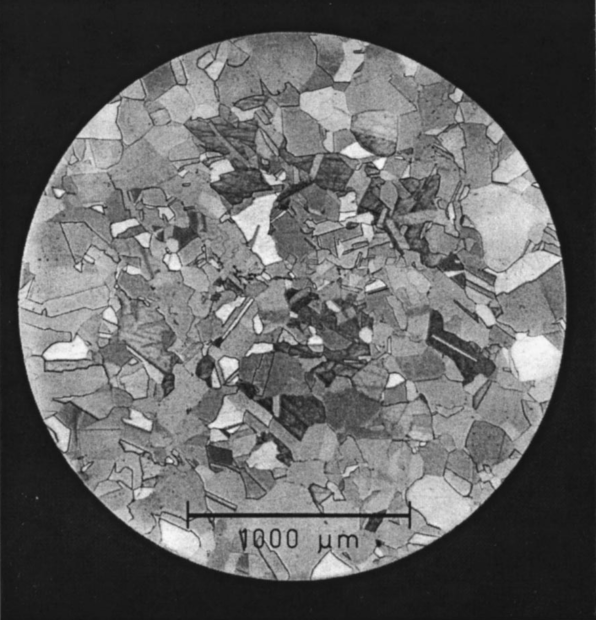
\includegraphics[width=0.4\textwidth]{Pictures/NiSphere.png}
	\caption{Cristalline structure of Nickel Sphere}
	\label{fig:NiSphere}
\end{figure}

We calculated afterwards its magnetic moment in the VSM. Figure \ref{fig:VSMNiSphere} shows the result.\\

\begin{figure}[ht]
	\centering
  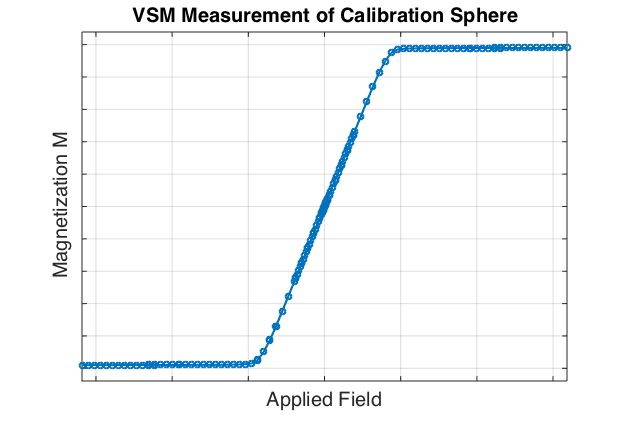
\includegraphics[width=0.8\textwidth]{Pictures/VSMNiSphere.png}
	\caption{Measurements of magnetic moment for a polycristalline nickel sphere}
	\label{fig:VSMNiSphere}
\end{figure}

A sphere always magnetizes uniformly for any kind of applied fields. Its demagnetization matrix therefore stays constant for low and high fields. Since, for high fields, the trace of the demagnetization matrix of any body sums up to   one, and a sphere is symmetric in all three directions the following holds:

\begin{equation}
N = \frac{1}{3}I
\end{equation}

For the same reason, the apparent susceptibility is the following:

\begin{equation}
\chi_a = \chi_{a,s}I
\end{equation}

Where $\chi_{a,s}$ is the slope of the curve until saturation (since it's a sphere, we would become that curve for every direction, therefore it stays constant). Writing down the definition of the apparent susceptibility and usign the demagnetization matrix for spheres, we get the following:

\begin{subequations}
\begin{equation}
\chi_a = \left(\frac{1}{\chi_m}I+N\right)^{-1}
\end{equation}
\begin{equation}
 \chi_{a,s}I = \left(\frac{1}{\chi_m}I+\frac{1}{3}I\right)^{-1}
\end{equation}
\end{subequations}

From which only one scalar equation remains relevant:

\begin{equation}
 \chi_{a,s} = \frac{1}{\frac{1}{\chi_m}+\frac{1}{3}}
\end{equation}

Which leads to the following:

\begin{equation}
 \chi_{m} = \frac{1}{\chi_{a,s}}-\frac{1}{3}
\end{equation}

In our measurements, the value was the following:

\begin{equation}
\chi_m \approx 24
\end{equation}


\subsection{Comparison with Simulations}

In the case of a perfect sphere, we saw from the graph, that the slope of the VSM measurement stays constant until its fully saturated. This is a special case which portrays the fact that the demagnetization matrix is constant for saturated as for non-saturated cases (since there is a unique algebraic transformation between $N$ and $\chi_a$. The interesting case, and crucial in this work, is to analyses and leave clear what happens for generic shapes (like helices) where the demagnetization matrix, and thus, the apparent susceptibility, is different for low fields as for high fields.\\

 To be more clear on this, lets analyze in FIgure \ref{fig:VSMExample} the graph of one example of the helices measured. Here we see, different than with the sphere, that the curve is not a constant slope that reaches saturation and then stays saturated, but rather goes smoothly from the unsaturated, linear case, to the saturated case. This case is very representative of the most general case and it leaves clear a very interesting point that is of core importance to the structure of this thesis: The apparent susceptibility, and therefore the demagnetization matrix, is dependent of the applied field and it is therefore of relevance to define the two limiting sections: low fields, when the slope is constant and high fields the exact point when the magnetization has reached a saturation point and it stays the same thereon.\\
 
 
 \begin{figure}[ht]
	\centering
  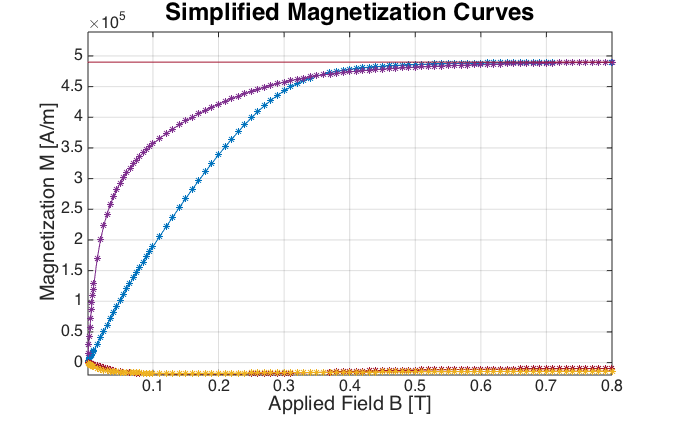
\includegraphics[width=0.8\textwidth]{Pictures/VSMExample.png}
	\caption{Calibrated VSM measurements of nickel macrohelix for positive applied fields. }
	\label{fig:VSMExample}
\end{figure}

 
 In the case of the sphere, the slopes are the same, but in the general case the challenge is to define both sections. The slope of the curve for low applied fields is not hard to find. As long as one takes small enough applied fields, a defined slope can be found for each curve. However, in the case of high fields, one has to define first the point where the saturation is reached and from that point on it stays saturated\footnote{May the reader be aware of this important convention: In this context, by slope, it is meant the slope of the line that goes from the origin to a certain point to the graph and not the slope in the sense of derivative}.\\
 
In order to be able to calculate the slopes of all curves to construct the apparent susceptibility and then the corresponding demagnetization matrix of each helix, we first have to do a meaningful definition of the point where the saturation happens, in order to calculate the slope at this point.\\
    
\begin{figure}[ht]
	\centering
  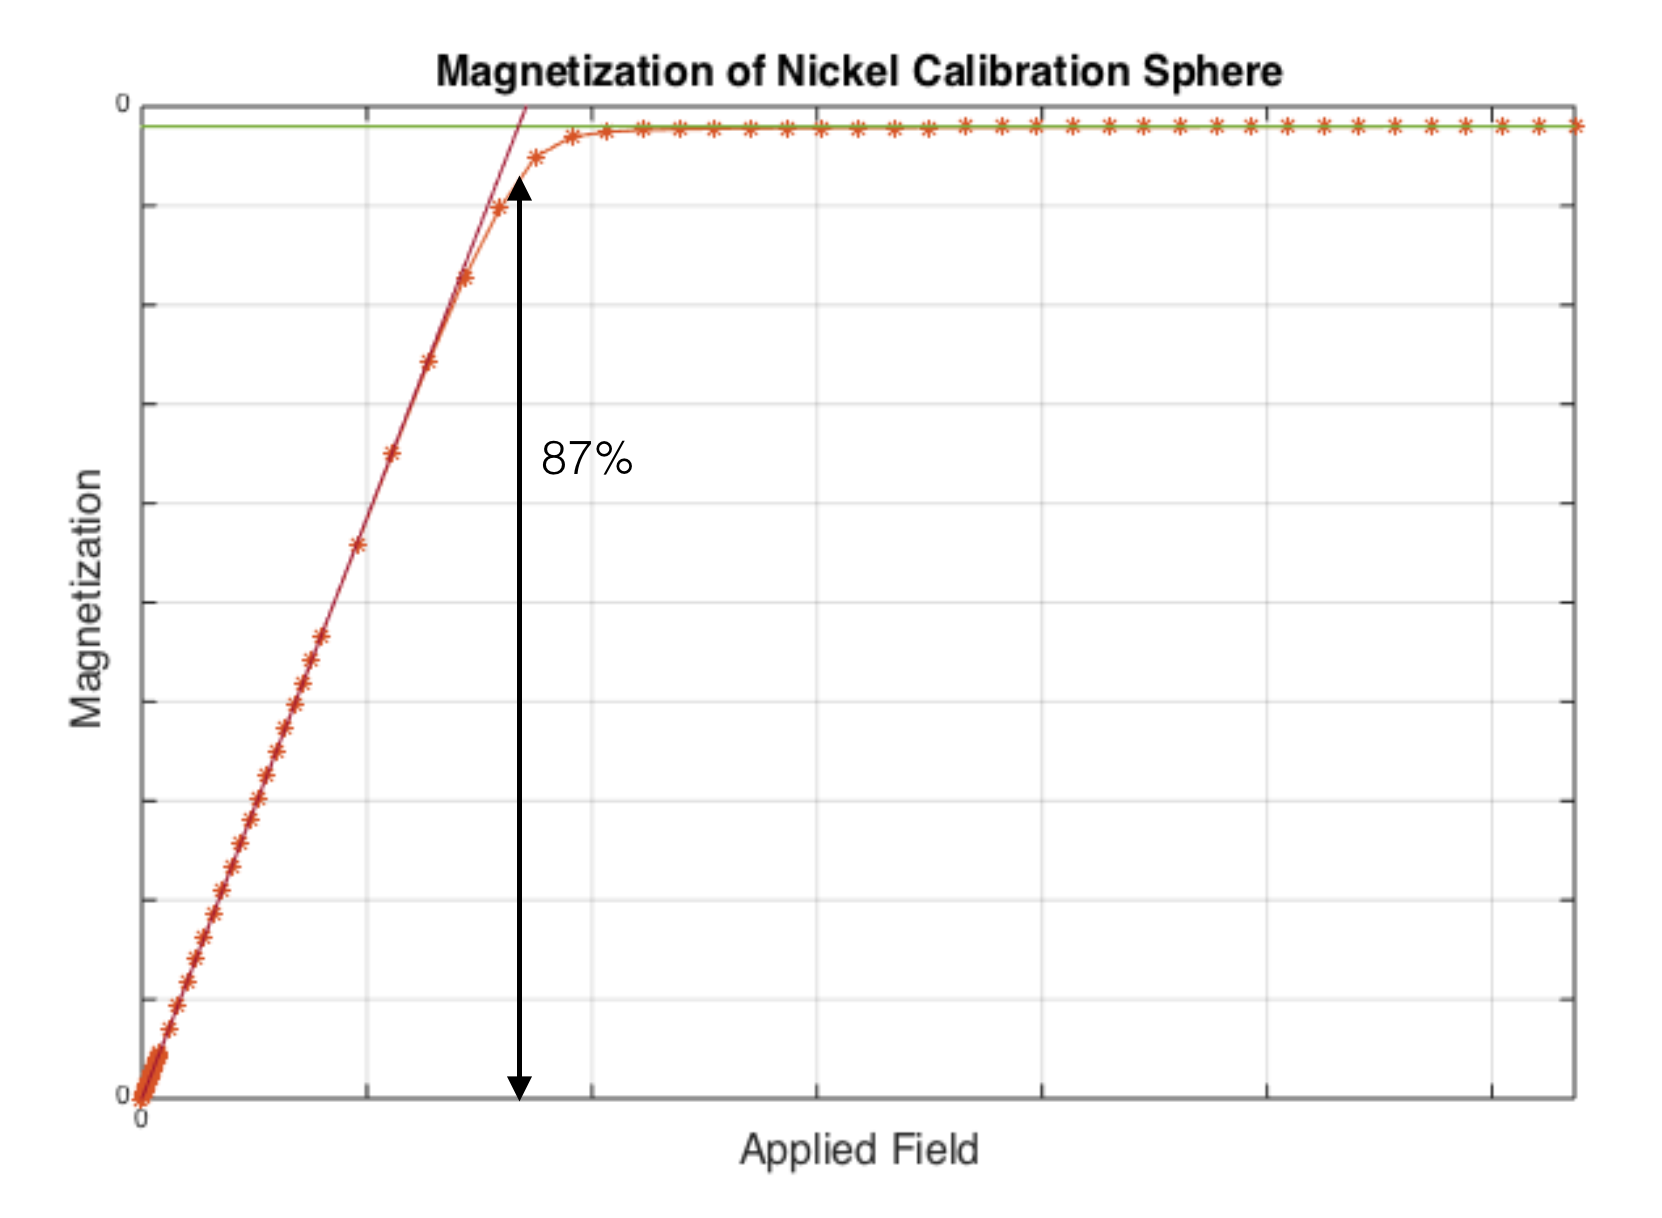
\includegraphics[width=0.8\textwidth]{Pictures/NiSphere_2.png}
	\caption{Measurements of magnetic moment for a polycrystalline nickel sphere with linearized trends}
	\label{fig:NiSphere_2}
\end{figure}

FIgure \ref{fig:NiSphere_2} shows the linearized trends of the low fields and the high field area of the nickel sphere. Ideally, since the nickel sphere is perfectly linear and magnetizes uniformly for any applied field, the demagnetization matrix and thus the apparent susceptibility (and thus the slope) should be constant until it saturates. Which means that the curve shouldn't be rounded, but rather stay perfectly linear until it saturates and then stay that way. In other words, the curve should never stop touching the trend lines.\\

The fact that this curve is not as it should in theory, can be used as criteria to do a quantitative comparison of how the real life case behaves compared to the theoretic one. In this case, we calculate the applied field in order for the theoretical curve to saturate, and then we calculate the percentage of saturation the actual curve actually achieves at this applied field. In this case, the ratio was $r = 87\%$.\\

This percentage will serve us as our criterium to analize and define saturation for the other helices. In other words, we will define the saturation point at the applied field, where the actual curve reaches $87\%$ of the saturation line for that specific helix. When doing that we will be able to calculate the slope of every curve and thus, the apparent susceptibility matrix of each helix and thus its demagnetization matrix, which we will then calculate with the simulations. \\


In Figure \ref{fig:NiHelix_Slopes} we see for $k = 2$ how the helix magnetization curves look like with the low field slopes as well as the saturation (high field) slopes defined there, where the curve achieves $r = 87\%$ of its saturation. For a complete assessment which includes all curves and calculations of demagnetization matrices and apparent susceptibilities please refer to Appendix \ref{s:ExperimentalResults}.\\

\begin{figure}[ht]
	\centering
  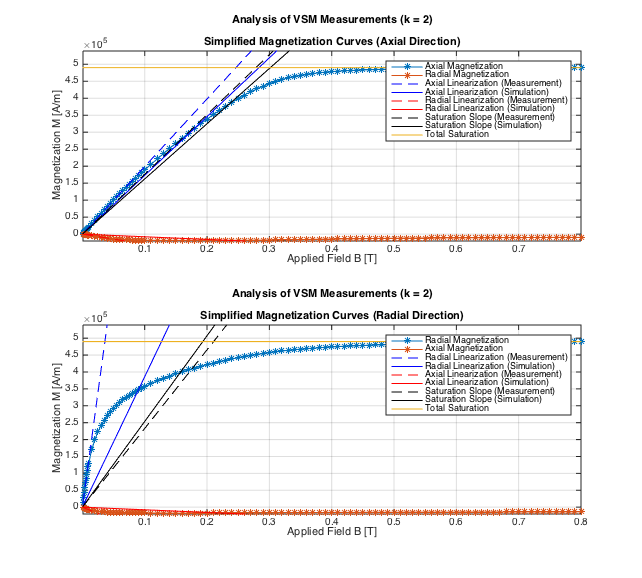
\includegraphics[width=1\textwidth]{Pictures/NiHelix_Slopes.png}
	\caption{Measurements of magnetic moment for a polycrystalline nickel helix with linearized trends (k = 2) and comparison with the simulated helices}
	\label{fig:NiHelix_Slopes}
\end{figure}

After analyzing the demagnetization matrices we see see that for $k=2, 3$ and $4$ we were able to capture the overall behavior of the magnetization for low and high fields. The easier axes to magnetize are the same in both results. For $k = 7$ the results are similar for low fields, but for high fields, we see a difference in the easier axes to magnetize between the simulation and the experiments. This is due to the fact that the diagonal values are very similar. \\

The results are satisfactory, considering the bold assumptions taken before. The factor contributing to the overall discrepancy between simulation and experiments could be not only human errors when coiling the macro helices, cutting them so the number of coiling turns is really a natural number and the alignment when putting the probe in the VSM, but also the assumption of same material composition between the sphere and the helices (which led to $r = 87\%$). \\

Also, one of the bold assumptions is the simplification of a hysteretic nonlinear curve to a single curve. Although the hysteresis is rather thing, the magnetization of the curve when magnetizing it from zero was not taken into consideration, but rather the complete loop curve, which was then averaged and centered such that it is a real symmetric curve that really crosses the origin. The major question would be, if this assumption is really meaningful, and it can only be answered depending of the application. Is the helix going to be re-magnetized or is it going to be magnetized from an absolutely neutral magnetization? These are questions that will have to be answered later depending on the specific application.


%!TEX root = thesis.tex
\section{Conclusion}

The original aim of this piece of research was to find the theoretical bridge between the two main areas of helical microrobots. The magnetic properties of them (in other words, how they magnetize under an applied field) and the fluid dynamics of the helical shape. Although, as it was shown in the Introduction, there is plenty of research that addresses both areas, there are few that really try to attack both at the same time trying to find an integral solution that allows to optimize the output (the movement of the robot itself) with its input, the rotating magnetic field.\\

Although it might seem that there is enough research on the magnetic properties of the helices, diving more in depth in the topic let us realize that there are some important gaps in the theory that have to be cleared out in order to have a clear view on how to tackle the original problem.\\

First of all, most of the recent research on the area of magnetism used tools and assumptions like the demagnetization matrix without questioning its real definition in the theory of magnetism. Therefore the first approach taken in this work, was to develop a theory that starts with the basic principles of electromagnetism and construct the solutions in order to arrive to the formal definition of the demagnetization matrix. This let us realize the first important part of this work, which is the differentiation of low fields and high fields. Most applications on microrobots involve low applied fields, but the few formal definitions of the demagnetization fields assumed magnetic saturation, which is only achieved with low field. The challenge then, was to prove, that there actually exists a demagnetization matrix for low fields. Although this might seem like an easy assumption, it was only possible to prove until the linearity properties of the derived integral equation were properly analyzed. Having set up a robust and clear theory for the demagnetization matrix for both separate cases, the low field case, and the saturated (high field) case we were able to dig more in depth in the practical calculations of these, checking consistency with existing research (for example with known shapes).\\

We already knew from existing research, that the demagnetization matrix for high fields is a 3D matrix surface integral to solve. The practical implementation of the evaluation of this integral was a numerical challenge that needed various mathematical manipulations (e.g. the conversion to a volume integral) to find the most suitable way. In this area we found that the best way of solving this numerically is performing a surface integral, avoiding this way the complications of the highly singular matrix kernel in the volume integral. The problem with this method is that, for each point in the helix, one has evaluate the surface nine 3D surface integrals, which makes the averaged demagnetization field a task which needs highly performing computers to perform. Optimizing the calculation of the averaged demagnetization matrix is a task to look more in depth in further research. Besides the challenges and the calculation intensity of this integrals, we were able to develop an integral method that showed close to equal results than the ones obtained through simulations\\

In the case of low fields, there is no research found on the calculation of demagnetization matrices through integral methods. The theory let us know that the demagnetization matrix (similar to the high fields case) is a 3D integral surface integral problem, this time one has to find the solution to an integral equation, for each point in the material. This poses a major calculation problem. We tried to dive deeper in the solving of this problem, specifically the solving of the integral equation. Unfortunately, the integrals used in the equation have a very complex and highly singular structure, that made the problem specially challenging. Through the experimentation with multiple methods, including the one we developed ourselves (shown previously) and unsatisfactory results, we decided to leave this problem for further research, since it needs sophisticated mathematical tools and methods specifically tailored for magnetic problems. For the theoretical results we had to rely on the simulations performed with FEM.\\

One of the most important parts in this work was doing FEM simulations in COMSOL. We validated some shapes were the demagnetization matrices were known algebraic expressions and we were able to confirm the correctness of the simulation environment. This allowed us to assume always the simulation environment as correct and as a reference to the closest match of the theoretical solution. Since the software was very intuitive and mature, it wasn't hard to deal with the different tools put to disposition and exploit the functionalities, also with the help of Matlab. The main problems encountered in the simulations were at the simulation of non-linear magnetic behavior, which led to convergence errors in the solvers at first. The other problem encountered was the meshing of the half coated since it is a very thin shape. Both problems were solved with the help of the support team of COMSOL. Besides that, finding a way of modeling in 3D the half coated shape for coiled indexes (H1.5 and below) was a major challenge that, even after several attempts, wasn't successful due to meshing problems. This will be left for further research.\\

Out of the demagnetization matrices we calculated for the helices H1 to H10 (low fields and high fields), we could calculate the misalignment angles for the helices and compare them to real measured data. We saw that we could clearly capture the trend of the curve. Taking in consideration practical factors like the influence of the wall (where the measurements were done) could help give a more realistic comparison.\\

After having settled clear the theoretical differences of the both cases, the saturated case and the low field case and having had the simulations as a reference point, a connection to the real case was needed. The need of real VSM measurements and the comparison to its simulated counterpart was to be analyzed to give the work done a deeper meaning. We manually coiled up 4 different macro helices and measured its (averaged) magnetization with the help of the VSM. We first used a calibration nickel sphere to have the real material properties of nickel. Our first realization was that, unlike most of the literature pieces that have dealt with this topic, the intrinsic susceptibility wasn't as high as we had assumed from the beginning on (the experiments showed that $\chi_m = 24$). We then created a simulation environment with this new intrinsic susceptibility.\\

The simulation part was not a big challenge since it was basically the same as it was used for the microhelices. Since the material we're using is polycrystalline and we're dealing with sizes much bigger than the sizes of the magnetic domains, therefore the material properties are the same in the macro case as in the micro case. The real challenge here was the evaluation of the measurements. It seems that we arrived at key questions that have not been asked often in the area of microhelices. We are dealing with a ferromagnetic helices with very complex properties that have to be simplified in meaningful ways. The magnetization of the helices happens in a hysteretic loop, that, although being thin, magnetizes in a different way the first time it magnetizes as it is after it is inside the loop. This is the reason why the question of how a helix magnetizes in low fields has no clear answer. Further research should put in context the environment in which the helices are going to be magnetized.In our case, we assumed that the helices are already in the magnetization loop (it is not the first time they magnetize) and therefore the first magnetization part was left unexamined and the loop was averaged such that only one clear function remains.\\

Another big challenge, encountered when analyzing the measurements, was to define the saturation point of the helices. Unlike the sphere, where this is a perfectly linear behavior that reaches saturation at a specific point and then stays that way (in theory, of course), the helices, in practice don't have a clear saturation part and therefore an assumption has to be made in terms of percentage of saturation achieved, which was taken from the measurements of the calibration sphere.\\

The results obtained from the simulation and the VSM measurements were satisfactory and gave a clear insight of correctness in terms of the easy axes and the qualitative diagonal values of the demagnetization matrices between each other. Of course a bold assumption was to take the same intrinsic susceptibility for the sphere as for the helices. In the future, a sphere with exactly the same material properties (composition and material) should be used for the intrinsic susceptibility. Further research should analyze more in depth a meaningful way of simplifying the measurements and other possible ways of defining the saturation point, which is crucial to get the correct values for the demagnetization matrices in high fields.\\

This thesis should serve as an important part for further research to complement the magnetic behavior of the helices and complement the theories that include both the magnetism theory and the fluid dynamical theory to optimize the response of applied fields towards the dynamic and kinetic properties of the helices. In the search of the optimal helix shape for our purposes it is still an early stage to chose an optimal shape before combining it with the fluid dynamical relations. We still saw an optimizable behavior in the demagnetization fields since the curves had global maxima and minima. Further research will have to analyze the behavior of the helices in a free unconstrained environment in presence of applied fields since in this thesis only constrained environments were considered. This should complement the search for an optimizable theory to find the optimal alignment and its comparison to the experiments.


%\include{SummaryAndContributions}

% Bibliography
\newpage\mbox{}\newpage
\addtocontents{toc}{\vspace{.5\baselineskip}}
\addcontentsline{toc}{section}{\protect\numberline{}{References}}
\bibliography{library}

\newpage\mbox{}\newpage
% Appendices (if needed)
\addtocontents{toc}{\vspace{.5\baselineskip}}
\appendix
%!TEX root = thesis.tex

\section{Manipulation of Demagnetization Integral Operator}
\label{s:Nmanipulation}


\begin{subequations}
\begin{equation}
\textbf{H}(\textbf{r})  = \frac{1}{4\pi}\int\limits_V\nabla\left(\frac{\textbf{r}-\textbf{r}'}{|\textbf{r}-\textbf{r}'|^3}\cdot\textbf{M}(\textbf{r}')\right)\;\mathrm{d}^3r'
\end{equation}
\begin{equation}
\textbf{H}(\textbf{r})  = \frac{1}{4\pi}\int\limits_V\left(\frac{\textbf{r}-\textbf{r}'}{|\textbf{r}-\textbf{r}'|^3}\cdot\textbf{M}(\textbf{r}')\right) \textbf{n}(\textbf{r}')\;\mathrm{d}^3r'
\end{equation}
\begin{equation}
\textbf{H}(\textbf{r})  = \frac{1}{4\pi}\int\limits_V\textbf{n}(\textbf{r}')\left(\frac{\textbf{r}-\textbf{r}'}{|\textbf{r}-\textbf{r}'|^3}\cdot\textbf{M}(\textbf{r}')\right)\;\mathrm{d}^3r'
\end{equation}
\begin{equation}
\textbf{H}(\textbf{r})  = \frac{1}{4\pi}\int\limits_V\textbf{n}(\textbf{r}')\left(\frac{\textbf{r}-\textbf{r}'}{|\textbf{r}-\textbf{r}'|^3}\cdot\textbf{M}(\textbf{r}')\right)\;\mathrm{d}^3r'
\end{equation}
\begin{equation}
\textbf{H}(\textbf{r})  = \frac{1}{4\pi}\int\limits_V\textbf{n}(\textbf{r}')\left(\frac{(\textbf{r}-\textbf{r}')}{|\textbf{r}-\textbf{r}'|^3}^T\textbf{M}(\textbf{r}')\right)\;\mathrm{d}^3r'
\end{equation}
\begin{equation}
\textbf{H}(\textbf{r})  = \frac{1}{4\pi}\int\limits_V\left(\textbf{n}(\textbf{r}')\frac{(\textbf{r}-\textbf{r}')}{|\textbf{r}-\textbf{r}'|^3}^T\right)\textbf{M}(\textbf{r}')\;\mathrm{d}^3r'
\end{equation}
\begin{equation}
\textbf{H}(\textbf{r})  = \frac{1}{4\pi}\int\limits_V\left(\frac{(\textbf{r}-\textbf{r}')}{|\textbf{r}-\textbf{r}'|^3}\textbf{n}(\textbf{r}')^T\right)^T\textbf{M}(\textbf{r}')\;\mathrm{d}^3r'
\end{equation}
\end{subequations}

Here we used the identity $\nabla(\textbf{u}\cdot\textbf{v}) = (\textbf{u}\cdot \nabla)\textbf{v} +  (\textbf{v}\cdot \nabla)\textbf{u} + \textbf{u}\times(\nabla\times\textbf{v}) + \textbf{v}\times(\nabla\times\textbf{u})$ as well as $\int\limits_V \nabla w \,d^3r'=  \oint\limits_{\partial V} w \textbf{n}\,d^2r'$ (for a scalar function $w$) and some simple matrix algebraic manipulations

\section{Proof of Linearity of Integral Equation}
\label{s:LinearityIntegralEquation}

For a specific helix and material we have the following integral equation:

\begin{equation}
\frac{1}{\chi_m}\textbf{M}(\textbf{r})  = -\mathcal{N}(\textbf{M}(\textbf{r})) + \textbf{H}_\text{app}
\end{equation}

We want to prove the linearity of the solution over the applied field. For this sake, we will make the dependance of the solution on the applied field explicit. The solution to this equation is therefore:

\begin{equation}
\textbf{M}(\textbf{r},\textbf{H}_\text{app})
\end{equation}

The next step is to prove linearity of $\textbf{M}(\textbf{r},\textbf{H}_\text{app})$ over $\textbf{H}_\text{app}$. We take first two cases: 


\begin{equation}\label{eq:case1}
\frac{1}{\chi_m}\textbf{M}(\textbf{r},\textbf{H}_\text{app,1})  = -\mathcal{N}(\textbf{M}(\textbf{r},\textbf{H}_\text{app,1})) + \textbf{H}_\text{app,1}
\end{equation}
\begin{equation}\label{eq:case2}
\frac{1}{\chi_m}\textbf{M}(\textbf{r},\textbf{H}_\text{app,2})  = -\mathcal{N}(\textbf{M}(\textbf{r},\textbf{H}_\text{app,2})) + \textbf{H}_\text{app,2}
\end{equation}

with solutions $\textbf{M}(\textbf{r},\textbf{H}_\text{app,1})$ and $\textbf{M}(\textbf{r},\textbf{H}_\text{app,2})$ respectively. By multiplying both equations with a real constant $\alpha$ and $\beta$ respectively and using the linear properties of the integral operator $\mathcal{N(\cdot)}$ it follows that:

\begin{equation}\label{eq:case1alpha}
\frac{1}{\chi_m}\alpha\textbf{M}(\textbf{r},\textbf{H}_\text{app,1})  = -\mathcal{N}(\alpha\textbf{M}(\textbf{r},\textbf{H}_\text{app,1})) + \alpha\textbf{H}_\text{app,1}
\end{equation}
\begin{equation}\label{eq:case2}
\frac{1}{\chi_m}\beta\textbf{M}(\textbf{r},\textbf{H}_\text{app,2})  = -\mathcal{N}(\beta\textbf{M}(\textbf{r},\textbf{H}_\text{app,2})) + \beta\textbf{H}_\text{app,2}
\end{equation}

by adding both equations and again using the algebraic and linearity properties of the integral operator (which has a matrix kernel) it follows that:

\begin{subequations}
\begin{equation}\label{eq:case1alpha}
\frac{1}{\chi_m}(\alpha\textbf{M}(\textbf{r},\textbf{H}_\text{app,1}) + \beta\textbf{M}(\textbf{r},\textbf{H}_\text{app,2}) )   = \end{equation}
\begin{equation}
 -\mathcal{N}(\alpha\textbf{M}(\textbf{r},\textbf{H}_\text{app,1}) + \beta\textbf{M}(\textbf{r},\textbf{H}_\text{app,2})) + (\alpha\textbf{H}_\text{app,1} + \beta\textbf{H}_\text{app,2})
\end{equation}
\end{subequations}

The solution to this is the magnetization field that results of the linear combination of the original fields which can be read clearly from the above equation:

\begin{equation}
\textbf{M}(\textbf{r},\alpha\textbf{H}_\text{app,1} + \beta\textbf{H}_\text{app,2}) = \alpha\textbf{M}(\textbf{r},\textbf{H}_\text{app,1}) + \beta\textbf{M}(\textbf{r},\textbf{H}_\text{app,2})
\end{equation}

Thus, linearity is proven.

\section{Derivation of Demagnetization Matrix for Low Fields}
\label{s:DemagPsi}

We want simplify the following equation:

\begin{equation}
N(\textbf{r}) := -H_d(\textbf{r})\,M(\textbf{r})^{-1}
\end{equation}

with: 

By using the following definitions:

\begin{subequations}
\begin{equation}
M(\textbf{r}) := [\textbf{M}_1(\textbf{r}), \textbf{M}_2(\textbf{r}), \textbf{M}_3(\textbf{r})]
\end{equation}
\begin{equation}
H_\text{app} := [\textbf{H}_{\text{app},1}, \textbf{H}_{\text{app},2}, \textbf{H}_{\text{app},3}]
\end{equation}
\begin{equation}
H_\text{d} := [\textbf{H}_{\text{d},1}, \textbf{H}_{\text{d},2}, \textbf{H}_{\text{d},3}]
\end{equation}
\end{subequations}

where:

\begin{equation}
\textbf{M}_i(\textbf{r}) = \Psi(\textbf{r})\textbf{H}_\text{app,i} \qquad i = 1,2,3
\end{equation}

and from the integral equation follows:


\begin{equation}
\textbf{H}_{d,i}(\textbf{r}) = \mathcal{N}(\textbf{r},\textbf{M}_i(\textbf{r}))\textbf{H}_\text{app,i} \qquad i = 1,2,3
\end{equation}

which simplifies to the following\footnote{Using our integral equation $\frac{1}{\chi_m}\Psi(\textbf{r}) = -\mathcal{N}(\textbf{r},\Psi(\textbf{r}))  + I$}:
\begin{equation}
\textbf{H}_{d,i}(\textbf{r}) = \left(\frac{1}{\chi_m}\Psi(\textbf{r})-I\right)\textbf{H}_\text{app,i} \qquad i = 1,2,3
\end{equation}

our tensor is now:

\begin{subequations}
\begin{equation}
N(\textbf{r}) := -H_d(\textbf{r})\,M(\textbf{r})^{-1} 
\end{equation}
\begin{equation}
 =- \left(\frac{1}{\chi_m}\Psi(\textbf{r})-I\right)H_\text{app} \left( \Psi(\textbf{r})H_\text{app}\right)^{-1}
\end{equation}
\begin{equation}
 = -\left(\frac{1}{\chi_m}\Psi(\textbf{r})-I\right)H_\text{app} H_\text{app}^{-1}\Psi(\textbf{r})^{-1}
\end{equation}
\begin{equation}
 = -\left(\frac{1}{\chi_m}\Psi(\textbf{r})-I\right)\Psi(\textbf{r})^{-1}
\end{equation}
\begin{equation}
 = -\left(\frac{1}{\chi_m}I-\Psi(\textbf{r})^{-1}\right)
\end{equation}
\begin{equation}
 = \Psi(\textbf{r})^{-1}-\frac{1}{\chi_m}I
\end{equation}
\end{subequations}

\clearpage

\section{Simulation Properties of Helices}

\subsection{Full magnetic}
\subsubsection{Geometry}

Description: Here, the geometry was created with the included COMSOL geometry for helices. (See Figure \ref{fig:COMSOLfull})

\begin{figure}[ht]
	\centering
  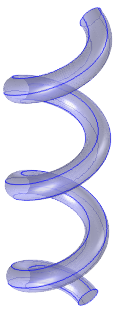
\includegraphics[width=0.15\textwidth]{Pictures/COMSOLfull.png}
	\caption{Example of 3D Geometry in COMSOL of Fully Magnetic Helix}
	\label{fig:COMSOLfull}
\end{figure}


Helix index: $n = 1,2,...,10$\\
Number of Coils: $k = 3$\\
Filament diameter: $d =  3\mu$m\\
Helix height: $h = h_\text{min} + (n -1)\frac{h_\text{max}-h_\text{min}}{9}$\\
Helix diameter: $D = \frac{1}{\pi}\sqrt{\left(\frac{4\cdot v_\text{nom}}{k\cdot \pi \cdot d_\text{nom}^2}\right)^2 - h^2}$\\\\
with:\\\\
$v_\text{nom} = \frac{1}{4}\pi \cdot d_\text{nom}^2 k \sqrt{h_\text{nom}^2+\pi\cdot D_\text{nom}^2} $\\
$d_\text{nom} = 3\mu$m\\
$D_\text{nom} = 10\mu$m\\
$h_\text{min} = 3\mu$m\\
$h_\text{max} = 32.97\mu$m\\
$h_\text{nom} = 10\mu$m

\subsubsection{Meshing Parameters}
COMSOL Predefined: Extremely fine

\subsection{Thin shell}
\subsubsection{Geometry}

Description: Here, the geometry was created with the included COMSOL geometry for helices. First a helix as created with the parametes below and afterwards an identical one with a filament diameter of $d = 3\mu\text{m} - 300$nm was substracted from it (See Figure \ref{fig:COMSOLthin}).

\begin{figure}[ht]
	\centering
  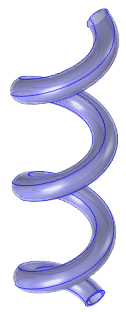
\includegraphics[width=0.15\textwidth]{Pictures/COMSOLthin.png}
	\caption{Example of 3D Geometry in COMSOL of Thin Coated Magnetic Helix}
	\label{fig:COMSOLthin}
\end{figure}

Helix index: $n = 1,2,...,10$\\
Number of Coils: $k = 3$\\
Filament diameter: $d =  3\mu$m\\
Helix height: $h = h_\text{min} + (n -1)\frac{h_\text{max}-h_\text{min}}{9}$\\
Helix diameter: $D = \frac{1}{\pi}\sqrt{\left(\frac{4\cdot v_\text{nom}}{k\cdot \pi \cdot d_\text{nom}^2}\right)^2 - h^2}$\\
Shell thickness: $s = 300$nm\\\\
with:\\\\
$v_\text{nom} = \frac{1}{4}\pi \cdot d_\text{nom}^2 k \sqrt{h_\text{nom}^2+\pi\cdot D_\text{nom}^2} $\\
$d_\text{nom} = 3\mu$m\\
$D_\text{nom} = 10\mu$m\\
$h_\text{min} = 3\mu$m\\
$h_\text{max} = 32.97\mu$m\\
$h_\text{nom} = 10\mu$m

\subsubsection{Meshing Parameters}
COMSOL Predefined: Extremely Fine

\subsection{Half Coated shell}
\subsubsection{Geometry}

Description: Here, the geometry was created with the included COMSOL geometry for helices. First a helix with its main axis pointing in z-direction was created with the parametes below and afterwards an identical one with shifted in negative x-direction by $s = 300$nm (See Figure \ref{fig:COMSOLhalf})

\begin{figure}[ht]
	\centering
  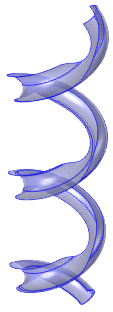
\includegraphics[width=0.15\textwidth]{Pictures/COMSOLhalf.png}
	\caption{Example of 3D Geometry in COMSOL of Half Coated Magnetic Helix}
	\label{fig:COMSOLhalf}
\end{figure}

Helix index: $n = 1,2,...,10$\\
Number of Coils: $k = 3$\\
Filament diameter: $d =  3\mu$m\\
Helix height: $h = h_\text{min} + (n -1)\frac{h_\text{max}-h_\text{min}}{9}$\\
Helix diameter: $D = \frac{1}{\pi}\sqrt{\left(\frac{4\cdot v_\text{nom}}{k\cdot \pi \cdot d_\text{nom}^2}\right)^2 - h^2}$\\
Shift factor: $s = 300$nm\\\\
with:\\\\
$v_\text{nom} = \frac{1}{4}\pi \cdot d_\text{nom}^2 k \sqrt{h_\text{nom}^2+\pi\cdot D_\text{nom}^2} $\\
$d_\text{nom} = 3\mu$m\\
$D_\text{nom} = 10\mu$m\\
$h_\text{min} = 3\mu$m\\
$h_\text{max} = 32.97\mu$m\\
$h_\text{nom} = 10\mu$m

\subsubsection{Meshing parameters}
\begin{tabular}{ | l | l | l | l | l | l | }
\hline
	h & Maximum & Minimum & Maximum   & Curvature  & Resolution \\ 
	 &  element &  element &  element   &  factor & of narrow  \\
	 &   size: &   size: &  growth rate: &   &  regions: \\ \hline
	1.5 & 1.37 & 1.71 & 1.45 & 0.5 & 0.6 \\ \hline
	1.65 & 1.44 & 1.81 & 1.45 & 0.5 & 0.6 \\ \hline
	1.75 & 1.56 & 1.95 & 1.45 & 0.5 & 0.6 \\ \hline
	1.9 & 1.69 & 2.12 & 1.45 & 0.5 & 0.6 \\ \hline
	2 & 1.77 & 2.21 & 1.45 & 0.5 & 0.6 \\ \hline
	2.2 & 1.93 & 2.41 & 1.45 & 0.5 & 0.6 \\ \hline
	2.3 & 2.33 & 2.91 & 1.45 & 0.5 & 0.6 \\ \hline
	2.35 & 2.33 & 2.91 & 1.45 & 0.5 & 0.6 \\ \hline
	2.45 & 2.33 & 2.91 & 1.45 & 0.5 & 0.6 \\ \hline
	2.55 & 2.33 & 2.91 & 1.45 & 0.5 & 0.6 \\ \hline
	2.6 & 2.33 & 2.91 & 1.45 & 0.5 & 0.6 \\ \hline
	2.7 & 2.33 & 2.91 & 1.45 & 0.5 & 0.6 \\ \hline
	2.8 & 2.33 & 2.91 & 1.45 & 0.5 & 0.6 \\ \hline
	3 & 2.33 & 2.91 & 1.45 & 0.5 & 0.6 \\ \hline
	3.2 & 2.33 & 2.91 & 1.45 & 0.5 & 0.6 \\ \hline
	3.3 & 2.33 & 2.91 & 1.45 & 0.5 & 0.6 \\ \hline
	4 & 3.36 & 4.19 & 1.45 & 0.5 & 0.6 \\ \hline
	5 & 4.14 & 5.18 & 1.45 & 0.5 & 0.6 \\ \hline
	6 & 3.4 & 2.47 & 1.45 & 0.5 & 0.6 \\ \hline
	7.2 & 5.87 & 7.34 & 1.45 & 0.5 & 0.6 \\ \hline
	8 & 6.49 & 8.11 & 1.45 & 0.5 & 0.6 \\ \hline
	9.1 & 7.4 & 9.25 & 1.45 & 0.5 & 0.6 \\ \hline
	10 & 7.95 & 9.94 & 1.45 & 0.5 & 0.6 \\ \hline
\end{tabular}

\clearpage

\section{Assumption Assessment of Averaged Demagnetization Field for Low Applied Fields}
\label{s:NMComparison}

We want to analyse in depth the two averaging cases of the demagnetization field for low applied fields by using the matrix formulation:

\begin{equation}
N(\textbf{r}) = \Psi(\textbf{r})^{-1} - \frac{1}{\chi_m}I
\end{equation}

and 

\begin{equation}
\textbf{M}(\textbf{r}) = \Psi(\textbf{r})\textbf{H}_\text{app}
\end{equation}

and we insert it in both cases:

\begin{subequations}
\begin{equation}
\textbf{H}_{d,1} = -\langle N(\textbf{r})\rangle \langle \textbf{M}(\textbf{r})\rangle
\end{equation}
\begin{equation}
 = -\langle \Psi(\textbf{r})^{-1} - \frac{1}{\chi_m}I\rangle \langle \Psi(\textbf{r})\textbf{H}_\text{app} \rangle
\end{equation}
\begin{equation}
 = -\left(\langle \Psi(\textbf{r})^{-1}\rangle - \frac{1}{\chi_m}I\right) \langle \Psi(\textbf{r}) \rangle\textbf{H}_\text{app}
\end{equation}
\begin{equation}
 = -\left(\langle \Psi(\textbf{r})^{-1}\rangle  \langle \Psi(\textbf{r}) \rangle- \frac{1}{\chi_m} \langle \Psi(\textbf{r}) \rangle\right)\textbf{H}_\text{app}
\end{equation}
\end{subequations}
and
\begin{subequations}
\begin{equation}
\textbf{H}_{d,2} = - \langle N(\textbf{r})  \textbf{M}(\textbf{r})\rangle
\end{equation}
\begin{equation}
= - \langle\left( \Psi(\textbf{r})^{-1} - \frac{1}{\chi_m}I \right) \Psi(\textbf{r})\textbf{H}_\text{app}\rangle
\end{equation}
\begin{equation}
= - \langle\left( I - \frac{1}{\chi_m} \Psi(\textbf{r}) \right)\textbf{H}_\text{app}\rangle
\end{equation}
\begin{equation}
= -\left( I - \frac{1}{\chi_m}  \langle\Psi(\textbf{r})\rangle \right)\textbf{H}_\text{app}
\end{equation}
\end{subequations}

The following holds then
\begin{equation}
\textbf{H}_{d,1} \approx \textbf{H}_{d,2}  \Rightarrow \langle \Psi(\textbf{r})^{-1}\rangle  \langle \Psi(\textbf{r}) \rangle \approx I
\end{equation}

In order to assess how good the assumption is, one should further analyse the characteristics of the matrix function $\Psi(\textbf{r})$. Specifically the solutions of the matrix integral equation which describes it. This will be left for further research.

\clearpage

\section{Proof that $N$ and $\chi_a$ share eigenvalues}
\label{s:SameEigen}

We recall the relation between $N$ and $\chi_a$:

\begin{equation}
\chi_a = \left(\frac{1}{\chi_m}I+N\right)^{-1}
\end{equation}

Lets assume that $Q$ is the matrix that diagonalizes $N$ such that $N_\text{diag} = QNQ^{-1}$.

For try to diagonalize now the apparent susceptibility out with the same matrix $Q$:
\begin{subequations}
\begin{equation}
Q \chi_aQ^{-1} 
\end{equation}
\begin{equation}
=Q \left(\frac{1}{\chi_m}I+ N\right)^{-1}Q^{-1} 
\end{equation}
\begin{equation}
= Q\left[Q\left(\frac{1}{\chi_m}I+ N\right)\right]^{-1} 
\end{equation}
\begin{equation}
= Q\left(Q\frac{1}{\chi_m}I+ QN\right)^{-1} 
\end{equation}
\begin{equation}
= \left[\left(Q\frac{1}{\chi_m}I+ QN\right)Q^{-1}\right]^{-1} 
\end{equation}
\begin{equation}
= \left(Q\frac{1}{\chi_m}IQ^{-1}+ QNQ^{-1}\right)^{-1} 
\end{equation}
\begin{equation}
= \left(\frac{1}{\chi_m}QQ^{-1}+ QNQ^{-1}\right)^{-1} 
 \end{equation}
 \begin{equation}
 = \left(\frac{1}{\chi_m}I+ QNQ^{-1}\right)^{-1} 
 \end{equation}
 \begin{equation}
 = \left(\frac{1}{\chi_m}I+ N_\text{diag}\right)^{-1} 
 \end{equation}
\end{subequations} 
 
which is also a diagonal matrix. This means that $Q$ also diagonalizes $\chi_a$ and both matrices share eigenvalues.

\clearpage

\section{Experimental Assessment for Polycristalline Nickel Helices}
\label{s:ExperimentalResults}

\begin{figure}[h]
	\centering
  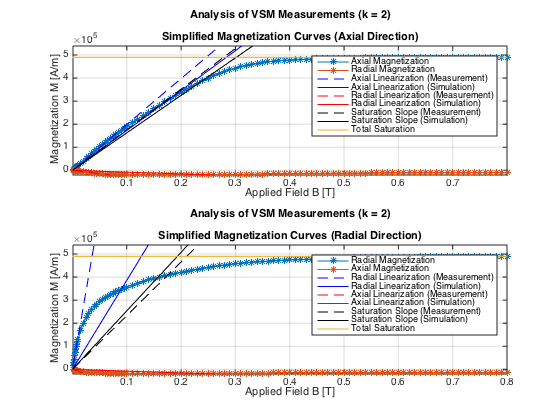
\includegraphics[width=1\textwidth]{Pictures/ExperimentalAssessk2.png}
	\caption{Comparison of simulation and experimental magnetization results for polycristalline nickel macrohelix (k = 2)}
	\label{fig:ExperimentalAssessk2}
\end{figure}

\begin{figure}[h]
	\centering
  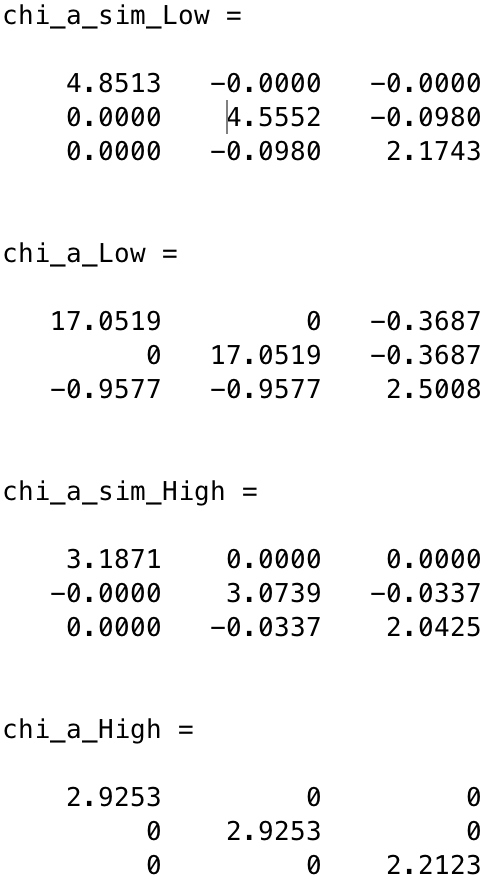
\includegraphics[width=0.25\textwidth]{Pictures/ExperimentalAssessk2chi.png}
	\caption{Comparison of simulation and experimental apparent susceptibilities for high and low fields for polycristalline nickel macrohelix (k = 2)}
	\label{fig:ExperimentalAssessk2chi}
\end{figure}

\begin{figure}[h]
	\centering
  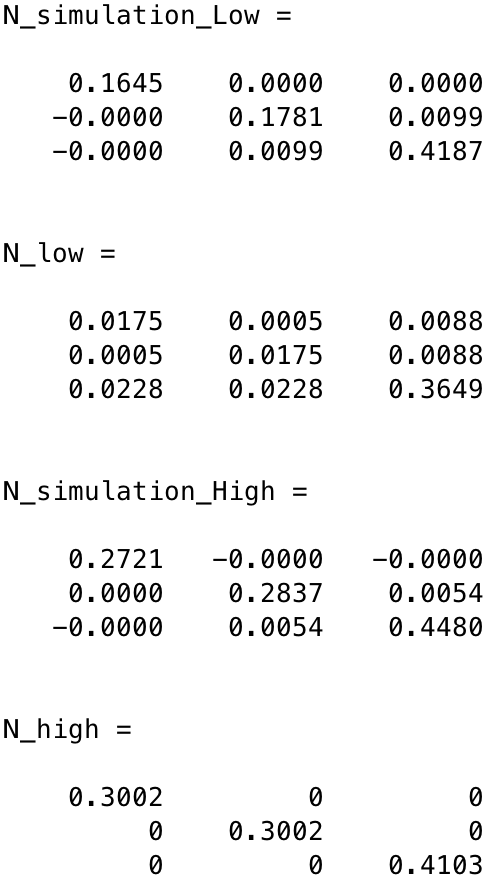
\includegraphics[width=0.25\textwidth]{Pictures/ExperimentalAssessk2N.png}
	\caption{Comparison of simulation and experimental demagnetization matrices for high and low fields for polycristalline nickel macrohelix (k = 2)}
	\label{fig:ExperimentalAssessk2N}
\end{figure}


\begin{figure}[h]
	\centering
  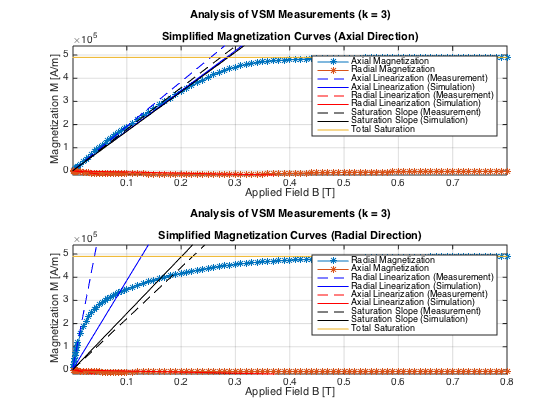
\includegraphics[width=1\textwidth]{Pictures/ExperimentalAssessk3.png}
	\caption{Comparison of simulation and experimental magnetization results for polycristalline nickel macrohelix (k = 3)}
	\label{fig:ExperimentalAssessk3}
\end{figure}

\begin{figure}[h]
	\centering
  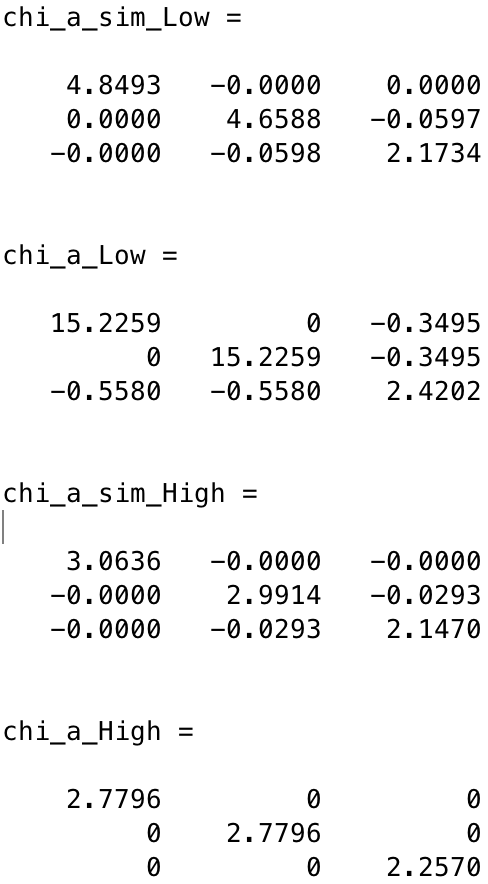
\includegraphics[width=0.25\textwidth]{Pictures/ExperimentalAssessk3chi.png}
	\caption{Comparison of simulation and experimental apparent susceptibilities for high and low fields for polycristalline nickel macrohelix (k = 3)}
	\label{fig:ExperimentalAssessk3chi}
\end{figure}

\begin{figure}[h]
	\centering
  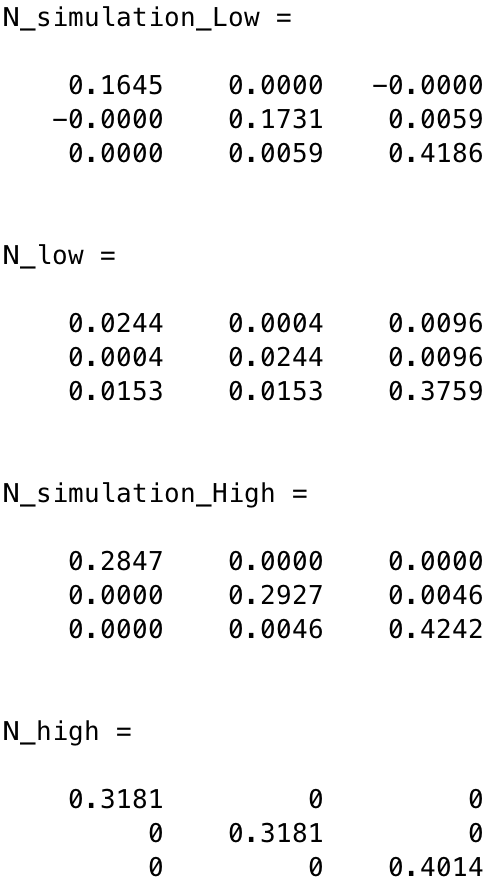
\includegraphics[width=0.25\textwidth]{Pictures/ExperimentalAssessk3N.png}
	\caption{Comparison of simulation and experimental demagnetization matrices for high and low fields for polycristalline nickel macrohelix (k = 3)}
	\label{fig:ExperimentalAssessk3N}
\end{figure}


\begin{figure}[h]
	\centering
  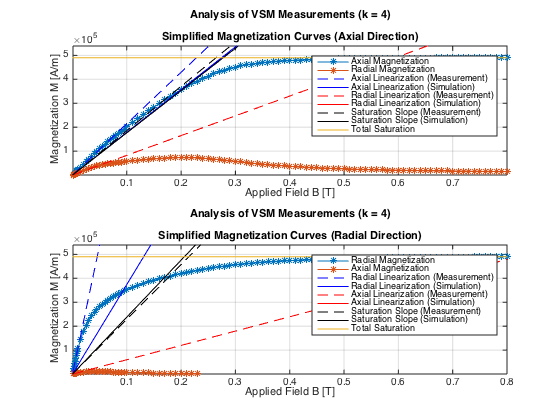
\includegraphics[width=1\textwidth]{Pictures/ExperimentalAssessk4.png}
	\caption{Comparison of simulation and experimental magnetization results for polycristalline nickel macrohelix (k = 4)}
	\label{fig:ExperimentalAssessk4}
\end{figure}

\begin{figure}[h]
	\centering
  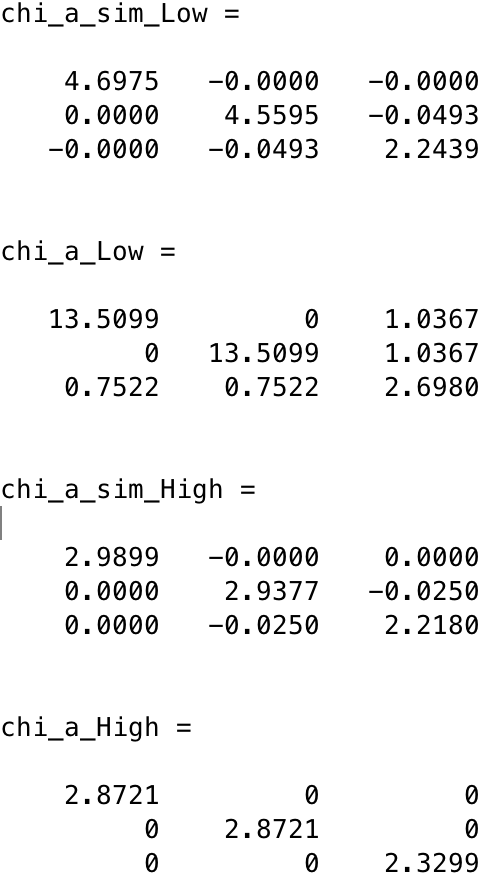
\includegraphics[width=0.25\textwidth]{Pictures/ExperimentalAssessk4chi.png}
	\caption{Comparison of simulation and experimental apparent susceptibilities for high and low fields for polycristalline nickel macrohelix (k = 4)}
	\label{fig:ExperimentalAssessk4chi}
\end{figure}

\begin{figure}[h]
	\centering
  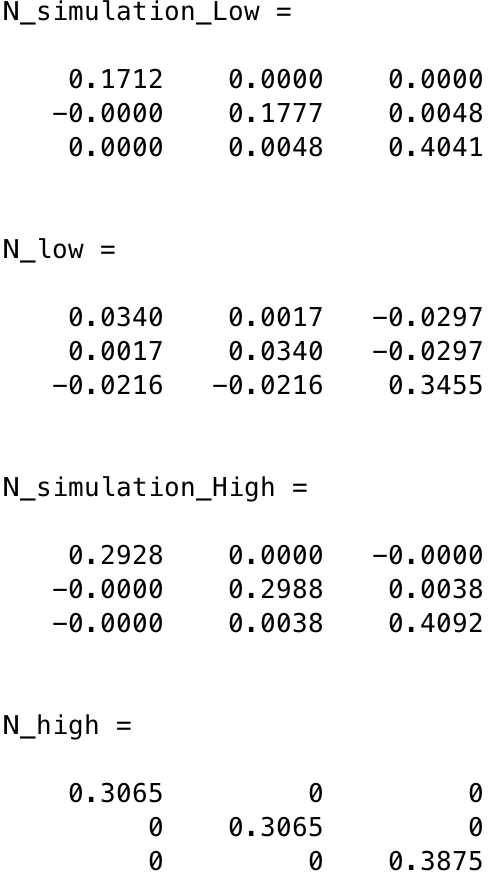
\includegraphics[width=0.25\textwidth]{Pictures/ExperimentalAssessk4N.png}
	\caption{Comparison of simulation and experimental demagnetization matrices for high and low fields for polycristalline nickel macrohelix (k = 4)}
	\label{fig:ExperimentalAssessk4N}
\end{figure}

\begin{figure}[h]
	\centering
  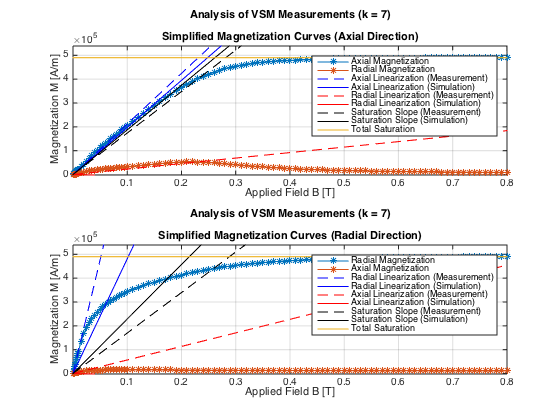
\includegraphics[width=1\textwidth]{Pictures/ExperimentalAssessk7.png}
	\caption{Comparison of simulation and experimental magnetization results for polycristalline nickel macrohelix (k = 7)}
	\label{fig:ExperimentalAssessk7}
\end{figure}

\begin{figure}[h]
	\centering
  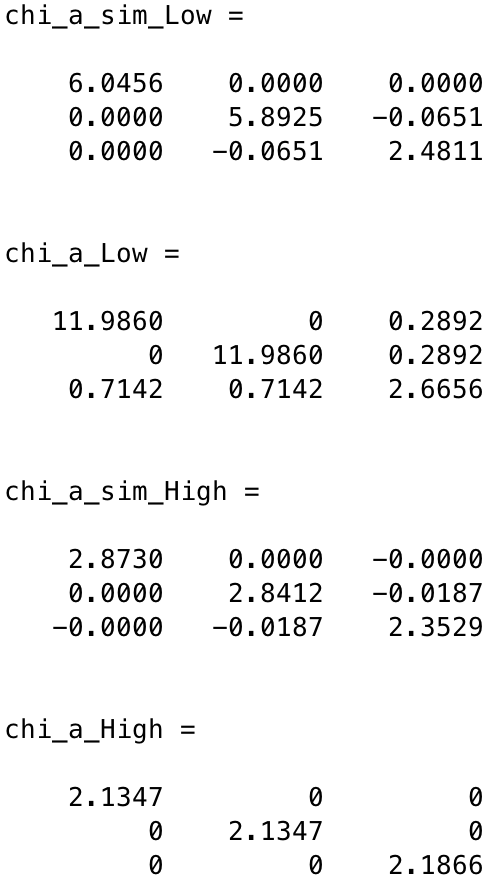
\includegraphics[width=0.25\textwidth]{Pictures/ExperimentalAssessk7chi.png}
	\caption{Comparison of simulation and experimental apparent susceptibilities for high and low fields for polycristalline nickel macrohelix (k = 7)}
	\label{fig:ExperimentalAssessk7chi}
\end{figure}

\begin{figure}[h]
	\centering
  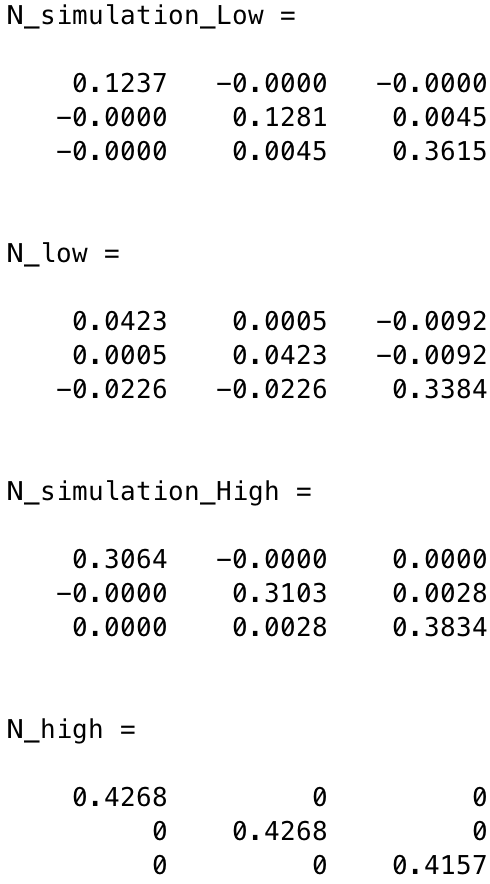
\includegraphics[width=0.25\textwidth]{Pictures/ExperimentalAssessk7N.png}
	\caption{Comparison of simulation and experimental demagnetization matrices for high and low fields for polycristalline nickel macrohelix (k = 7)}
	\label{fig:ExperimentalAssessk7N}
\end{figure}

\begin{figure}[h]
	\centering
  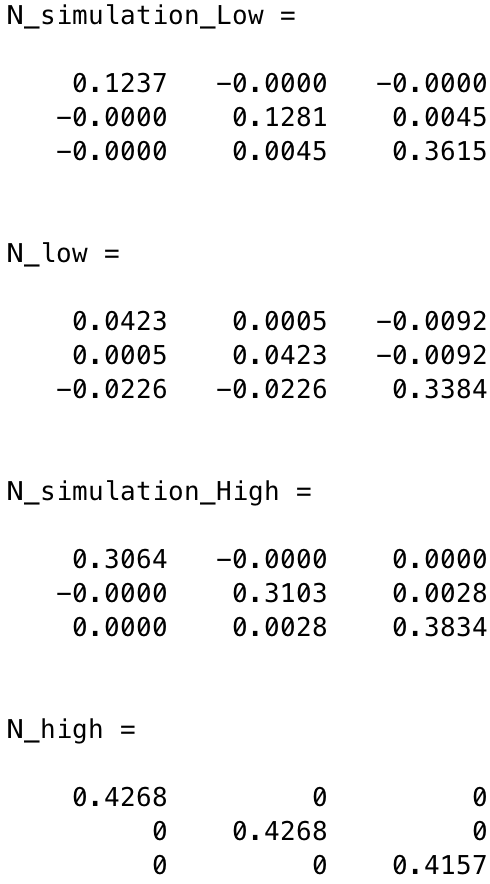
\includegraphics[width=0.25\textwidth]{Pictures/ExperimentalAssessk7N.png}
	\caption{Comparison of simulation and experimental demagnetization matrices for high and low fields for polycristalline nickel macrohelix (k = 7)}
	\label{fig:ExperimentalAssessk7N}
\end{figure}

\clearpage
\section{Setting up the simulation environment}

In this Section the three cases of simulations are going to be explained. The first two will be the means to the calculation of magnetic properties of a saturated magnetic shape. One setting up a fixed constant magnetization on the body, achieving this way an ideal saturation and skipping the step of actually magnetizing a shape and the second actually giving the body non-linear magnetic properties and subjecting it to very high fields. The third setup will be the simulation of low field magnetization, were we will give the body a linear magnetic property and then subject it to a field of some arbitrary magnitude. We will start by setting up the system for the shape and any magnetic calculations and we will go into the special details of every case separately.\\

\subsection{Adding the Physics}

We will start first by opening COMSOL and using the Model Wizard by clicking on ''New''. This part will help us set up the basics of the physics that are going to be used in COMSOL.\\

\begin{figure}[H]
	\centering
  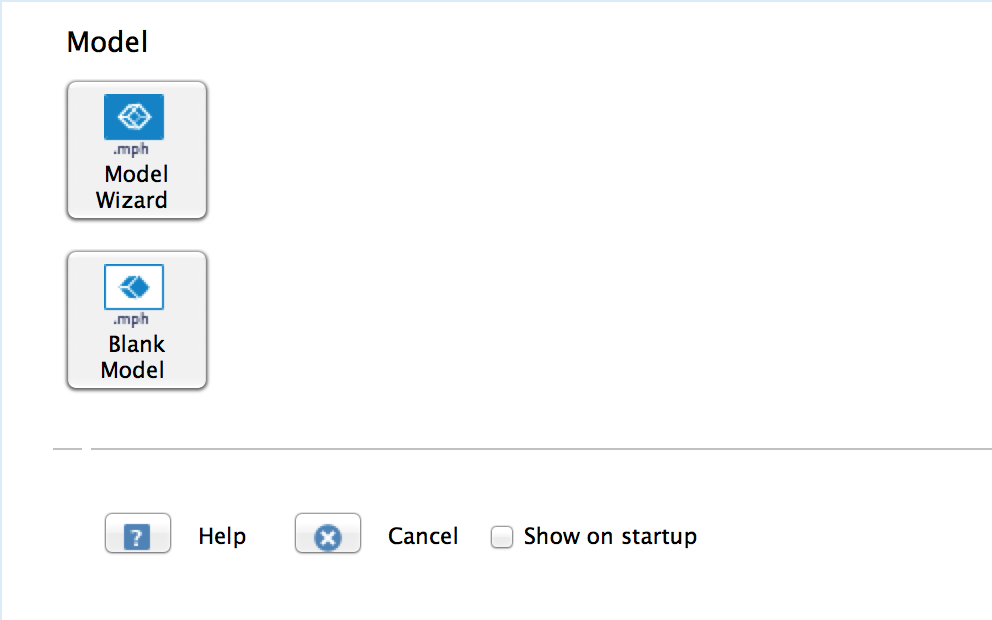
\includegraphics[width=0.6\textwidth]{Pictures/Screenshots/Sim1.png}
\end{figure}

After that, chose ''3D'' since we're going to be using a 3D model and simulation.\\

\begin{figure}[H]
	\centering
  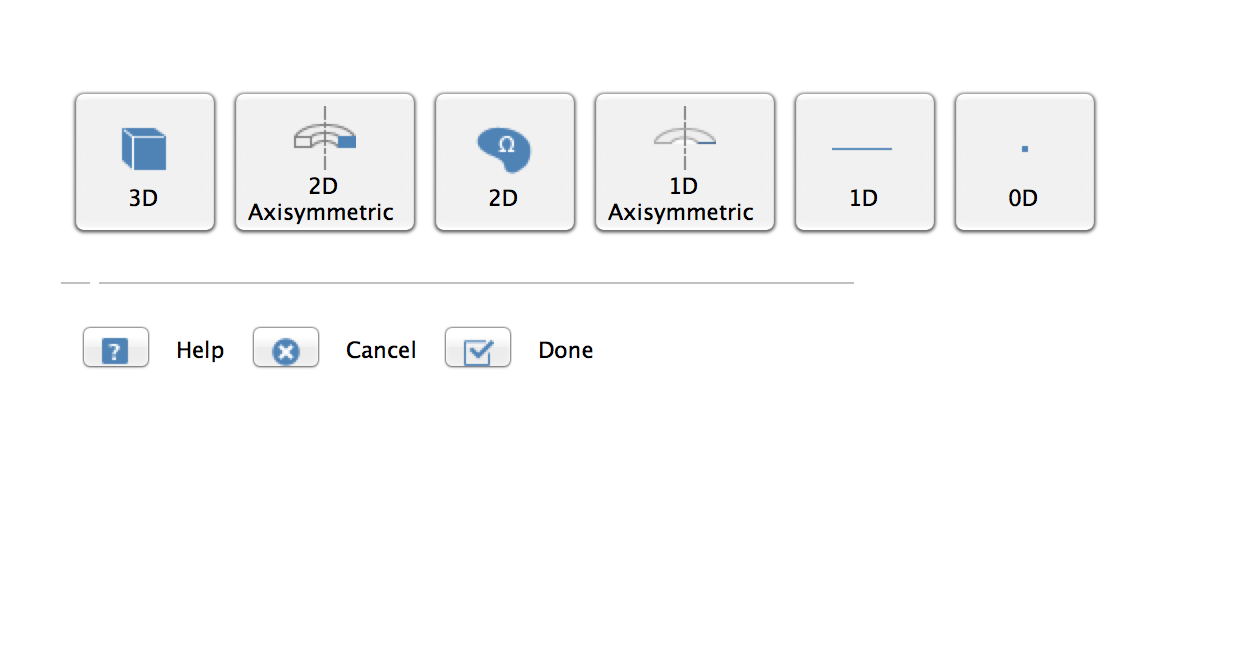
\includegraphics[width=0.6\textwidth]{Pictures/Screenshots/Sim2.png}
\end{figure}

The physics environment that is going to be used here is ''Magnetic fields, no currents (mfnc)''.\\

\begin{figure}[H]
	\centering
  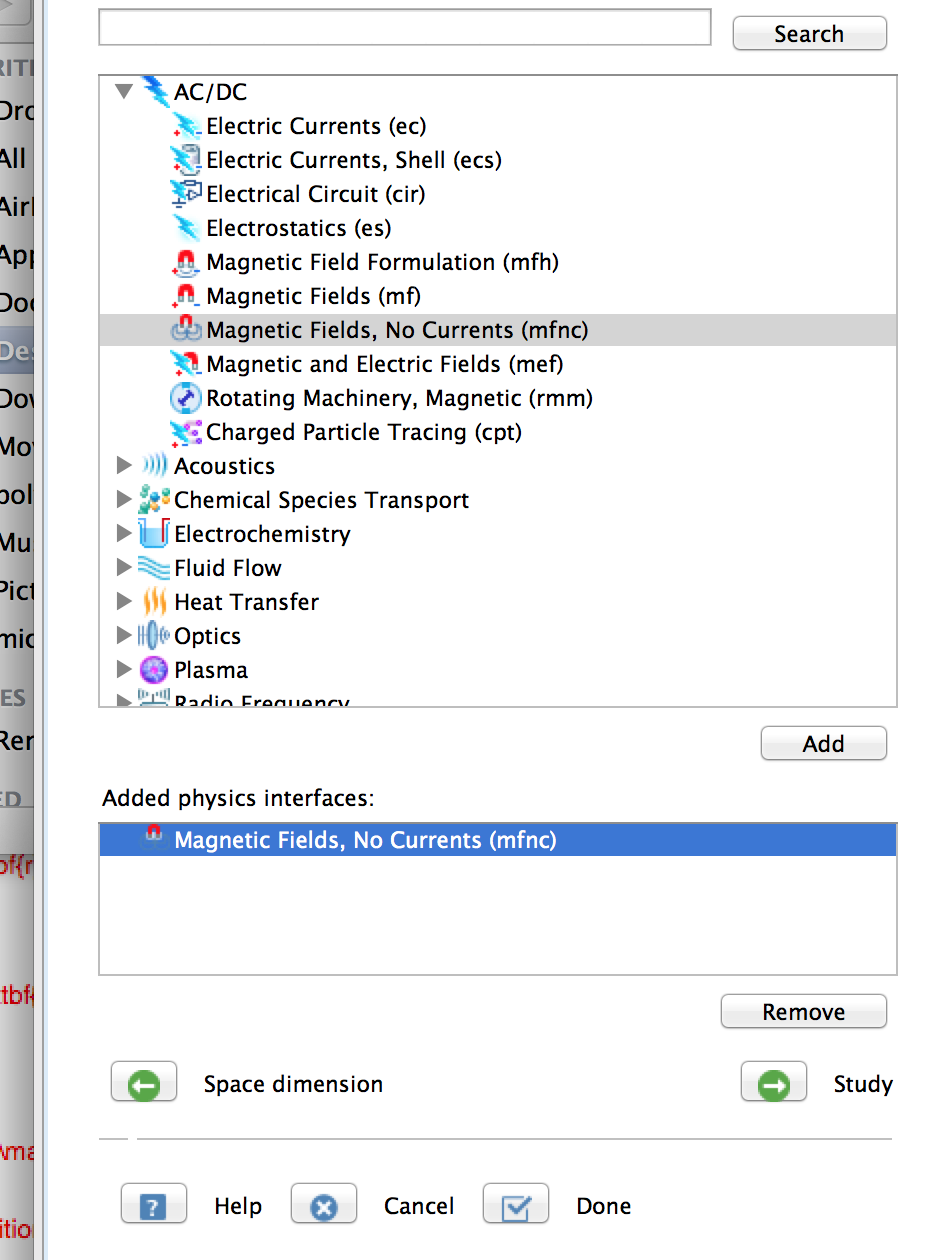
\includegraphics[width=0.4\textwidth]{Pictures/Screenshots/Sim3.png}
\end{figure}

Having this done, we continue by clicking on the ''Study'' button.\\

\begin{figure}[H]
	\centering
  \includegraphics[width=0.3\textwidth]{Pictures/Screenshots/Sim25.png}
\end{figure}

Here we chose the ''Sationary'' preset study and then we finish the wizard by clickin in  ''Done''.

\begin{figure}[H]
	\centering
  \includegraphics[width=0.4\textwidth]{Pictures/Screenshots/Sim4.png}
\end{figure}


\subsection{Adding the Geometry}

Adding the geomtry in COMSOL is a simple task that, as long as we're dealing with easy shapes or logical combinations (addition, substraction, etc.) of easy shapes, we can use the built-in functionalities of COMSOL. In this case we're going to show how to add a rectangular shape.\\

The first step is to go to the menu of Geometry by right-clicking on ''Geometry'' and selecting the desired Geometry, e.g. a helix or a block.\\

\begin{figure}[H]
	\centering
  \includegraphics[width=0.4\textwidth]{Pictures/Screenshots/Sim5.png}
\end{figure}

This done, the geometrical properties of the desired shape have to be edited and finally the button ''Build selected'' or ''Build all objects'' has to be clicked.\\

\begin{figure}[H]
	\centering
  \includegraphics[width=0.4\textwidth]{Pictures/Screenshots/Sim6.png}
\end{figure}

In order to our FEM simulations to be run successfully, one has to define a system boundary. This can be done by creating a shape, bigger than the objects to be analysed to sorround the geometries and define the limits. In this case we used a sphere with its radius being five times the longest axial dimension of the helix. \\

\begin{figure}[H]
	\centering
  \includegraphics[width=0.4\textwidth]{Pictures/Screenshots/Sim8.png}
\end{figure}

\subsection{Adding a material}

To add a material, one has to click on the ''Material'' node and select ''Add material''.\\
 \begin{figure}[H]
\centering
 \includegraphics[width=0.4\textwidth]{Pictures/Screenshots/Sim14.png}
\end{figure}

Then out of the material library (using the search bar) one selects the desired material. Since we're going to assume the environment is non-magnetizable we will chose ''Air'' and then assign it with the selection tool to the environment shape.\\

 \begin{figure}[H]
\centering
 \includegraphics[width=0.4\textwidth]{Pictures/Screenshots/Sim15.png}
\end{figure}

\subsection{Magnetization Environments}

In this we're going to show the set-up of the different environments used in this thesis. The first one being the constant magnetization to simulate a perfect saturated material, the second one the actual saturation of a non-linear magnetic shape through high fields and the last one the linear magnetization of the shape to simulate the low-field case.\\

Since this type of magnetization problems are solved through the scalar magnetic potential, it is convenient to define a zero-level for it to help the solvers work more efficiently (sparing, thus, the solver the decision of the zero placement in the 3D space). To do this we do a right-click on the node ''Magnetic Fields, No Currents (mfnc)'' and we select ''Zero Magnetic Scalar Potential''.\\

\begin{figure}[H]
	\centering
  \includegraphics[width=0.4\textwidth]{Pictures/Screenshots/Sim7.png}
\end{figure}

Once the object is created, using the selection tool, one can select any arbitrary point in the geometries created before.

\begin{figure}[H]
	\centering
  \includegraphics[width=0.4\textwidth]{Pictures/Screenshots/Sim9.png}
\end{figure}

 

\subsubsection{Linear Magnetization}

This will come first, since it's the easiest of the cases to set up. The only thing we have to do here is make sure that the relative permeability of the object is correct. By putting it in the correct field within the material selected for the shape\\
 
\begin{figure}[H]
	\centering
  \includegraphics[width=0.4\textwidth]{Pictures/Screenshots/Sim13.png}
\end{figure}

Having done this, one has to make sure, that the existing object ''Magnetic Flux Conservation'' has in the selection editor both the environment shape and the shape to magnetize inside.\\

After that we have to set-up the external applied field. To do this we create a new magnetic object called ''Magnetic Flux Density''.\\

\begin{figure}[H]
	\centering
  \includegraphics[width=0.4\textwidth]{Pictures/Screenshots/Sim17.png}
\end{figure}

Once created we make sure the environment shape is selected in the selection editor and then we change the picklist value ''Type'' to ''Magnetic Flux Density''. This being done, one can now chose the magnitude and direction of the applied external field under the title ''Magnetic Flux Density''.

\begin{figure}[H]
	\centering
  \includegraphics[width=0.4\textwidth]{Pictures/Screenshots/Sim18.png}
\end{figure}



\subsubsection{Constant Magnetization}

In this part we create a new magnetic object called ''Magnetic Flux Conservation''.\\

\begin{figure}[H]
	\centering
  \includegraphics[width=0.4\textwidth]{Pictures/Screenshots/Sim10.png}
\end{figure}
 
In the properties of this object we make sure only the shape to be magnetized is selected (using the selection editor on top) and then we change the value of ''Constitutive Relation'' by selecting the picklist value ''Magnetization''. In the fields for the remanent magnetization we select a magnetization value for each direction to get our magnetized shape. \\

\begin{figure}[H]
	\centering
  \includegraphics[width=0.4\textwidth]{Pictures/Screenshots/Sim11.png}
\end{figure}
 
 In this part there is no need for chosing any materials for the shape as well as an external applied field since we're dealing with the situation as if the magnetization (saturation) would already have happened.
 
\subsubsection{Saturation}

Starting from the same point we started in the section of Constant Magnetization, we have to create again the magnetic object 'Magnetic Flux Conservation''. We make sure, first, from the selection editor, that the right shape is chosen, namely the one that is going to get magnetized. This time we change the value of ''Constitutive Relation'' by selecting the picklist value ''BH Curve''. A new picklist appears with the name ''Magnetic flux density norm'' and its value has to be `'From Material''

\begin{figure}[H]
	\centering
  \includegraphics[width=0.4\textwidth]{Pictures/Screenshots/Sim12.png}
\end{figure}

No we have to make sure that the material has the right magnetization curve (BH Curve) so that the simulation is correct. For that we go to the material node and create a new material. In the material library we go to the Non-linear magnetic section and select any material of our choice.\\

 \begin{figure}[H]
	\centering
  \includegraphics[width=0.4\textwidth]{Pictures/Screenshots/Sim16.png}
\end{figure} 

The reason for this freedom of choice is only that we want to saturate the material. The curve itself, doesn't really interest us, but we rather just need the saturation behaviour to do our calculations, since we want to calculate the demagnetization factor (which is a shape factor).\\

What is now left is to create the applied field the way it was created in the section for Linear Magnetization this time making sure the magnitude of the field is big enough, e.g. 5000 Tesla.

\subsection{Meshing}

To create a Mesh node one has to do a right click on the Component node and click on ''Add Mesh''.

 \begin{figure}[H]
	\centering
  \includegraphics[width=0.4\textwidth]{Pictures/Screenshots/Sim19.png}
\end{figure} 

 The meshing properties of the environment and the meshing properties of the shape itself. To set this up one has to create the following objects in the Mesh node (by doing a right click on it): One size object and two ''Free Tetrahedral'' objects at the same level of the hierarchy and one ''Size'' object inside the second ''Free Tetrahedral'' object

 \begin{figure}[H]
	\centering
  \includegraphics[width=0.4\textwidth]{Pictures/Screenshots/Sim20.png}
\end{figure} 

For the meshing process there is two decisions that have to be made. The refinement of the mesh for the environment and the refinment of the mesh for the shape. For it to have the proper assignments the properties have to be set as shown in the illustrations. \\

For the first ''Size object'':\\
 \begin{figure}[H]
	\centering
  \includegraphics[width=0.4\textwidth]{Pictures/Screenshots/Sim21.png}
\end{figure} 


For the first ''Free Tetrahedral'' object:\\
 \begin{figure}[H]
	\centering
  \includegraphics[width=0.4\textwidth]{Pictures/Screenshots/Sim22.png}
\end{figure} 


For the second ''Size'' object\\
\begin{figure}[H]
	\centering
  \includegraphics[width=0.4\textwidth]{Pictures/Screenshots/Sim23.png}
\end{figure} 

For the second ''Free Tetrahedral'' object:\\
\begin{figure}[H]
	\centering
  \includegraphics[width=0.4\textwidth]{Pictures/Screenshots/Sim24.png}
\end{figure} 

\subsection{Calculating}

To activate the simulation one will have to do a right click on the ''Study'' node and click on ''Compute''.

\begin{figure}[H]
	\centering
  \includegraphics[width=0.4\textwidth]{Pictures/Screenshots/Sim26.png}
\end{figure} 


\subsubsection{Parametric Sweeps}

Since for our calculations we will need to do always a simulation for three linearly independent directions, we will need the functionality of Parametric Sweeps to work efficiently. This allows us to calculate the three directions within the same process and then export them to Matlab as one single process (instead of three).\\

The way to set it up is to create a ''Parametric Sweep'' object from within the ''Study Node''.\\
\begin{figure}[H]
	\centering
  \includegraphics[width=0.4\textwidth]{Pictures/Screenshots/Sim27.png}
\end{figure} 

The next step is to chose the variable or variables that have to change value in each of the different processes. In this case we chose the variables $B_x$, $B_y$ and $B_z$ defined in the global parameters and we assign the values they have to have in each of the processes in the following way:\\

\begin{figure}[H]
	\centering
  \includegraphics[width=0.4\textwidth]{Pictures/Screenshots/Sim28.png}
\end{figure} 

The variables are then put in the fields for the applied field within the ''Magnetic Flux Density'' object.\\
\begin{figure}[H]
	\centering
  \includegraphics[width=0.4\textwidth]{Pictures/Screenshots/Sim28.png}
\end{figure} 

It is important to know that Parametric Sweeps are a very powerful tool that allows to nest various Parametric Sweeps within each other in case one wants to do, for example, this type of calculation for three different directions at the same time for various different shape parameters (like in the case of the helices). In this case the parameter to be changed from cycle to cycle has to be defined the way the variables were defined in the above case and one would nest one Parametric Sweep inside the other.

\subsection{Postprocessing in Matlab}

In this module we will show the most important functionalities to import solutions of magnetic simulations from COMSOL into Matlab, such that the rest of the calculations and plotting (postprocessing) can be done in Matlab.\\

The first step to do is to open the COMSOL Multiphysics Server before Matlab is opened.\\

\begin{figure}[H]
	\centering
  \includegraphics[width=0.2\textwidth]{Pictures/Screenshots/Sim30.png}
\end{figure} 

Doing this, the terminal will open and will confirm if the server could have been opened and in which port it is listening (usually port 2036):

\begin{figure}[H]
	\centering
  \includegraphics[width=0.8\textwidth]{Pictures/Screenshots/Sim31.png}
\end{figure} 

The first line that has to be input in Matlab (only one time) is \textit{mphstart(2036)} where the number inside has to be the same one given in the terminal console. This will initializate the connection between the COMSOL environment and Matlab.

\begin{figure}[H]
	\centering
  \includegraphics[width=0.2\textwidth]{Pictures/Screenshots/Sim32.png}
\end{figure} 

After this one has to load the already simulated model to Matlab. To have a view of the nodes inside the loaded model one can always use the \textit{mphnavigator} to see them whithin Matlab, so there is no necesity of opening the model in COMSOL.

\begin{figure}[H]
	\centering
  \includegraphics[width=0.7\textwidth]{Pictures/Screenshots/Sim33.png}
\end{figure} 

Once the model has been loaded, the solutions within the model can be downloaded. Since we're dealing with averaged values over the whole shape we use the function \textit{mphmean}. The first argument refers to the previously loaded model. The second argument is a list of the variables (including solution variables) to be extracted from the models. These are extracted to the function outputs at the beginning of the line. The third argument states we are dealing with a volume average over the selection 2, which is the magnetized shape (selection 1 would be the environment sphere) the following two arguments state the selection of the dataset used (coming from the solution). To see the data set that is being used, one has to look it up in the solution node of the \textit{mphnavigator}. The last two inputs state the index of the solution within the outermost parameter sweep (in case there is one). In the case of having two Parameter Sweeps, this would refer to the outmost and the rest of the exported variables would have three values according to each one of the solutions (for each direction of the applied field).\\

\begin{figure}[H]
	\centering
  \includegraphics[width=\textwidth]{Pictures/Screenshots/Sim34.png}
\end{figure} 

Once this is done the matrices of the applied field (in this case zero, since we're dealing with the method were the magnetization is set as constant), the magnetization and the total H-field can be constructed according to the way it was defined in this thesis and then further calculations can be done. 

\section{Running Matlab Scripts with BRUTUS}

Before one uses BRUTUS, one has to contact the administrator to be sure to have an account on it. It is also recommended to have a FTP client (e.g. Filezilla) to manage the files in BUTUS. Provided this, one can continue with the specific steps.\\

Provided one is connected to the ETH network, either through wireless or through VPN, one can connect to the cluster with the next line:\\

\textit{ssh [username]@brutus@ethz.ch}\\

After having entered the password, te connection will have been set up properly

\begin{figure}[H]
	\centering
  \includegraphics[width=\textwidth]{Pictures/Screenshots/Sim35.png}
\end{figure} 

The next step is to load the Matlab module to be able to run Matlab scripts. For this one should use the line:\\

\textit{module load matlab}\\

Having this done. The important step now is to get the files to the server using a ftp manager. The direction is:\\

\textit{sftp://[username]@brutus.ethz.ch}\\

It is important to know the folder hierarchy within the sftp so that you know how to access it with unix commands through the command screen.

\begin{figure}[H]
	\centering
  \includegraphics[width=\textwidth]{Pictures/Screenshots/Sim36.png}
\end{figure} 

If, for example, I have my scripts under the folder called ''Calculations'' I type:\\

\textit{cd Calculations}\\

in the command line and then \textit{ls} to see the files within that folder. Once that one is in the desired folder one can send the job in the following way:\\

\textit{bsub -W "24:00" -R "rusage[mem=1500]" matlab -nodisplay -nojvm -singleCompThread -r simulation}\\

Where \textit{-W "24:00"} sets the time limit as 24 hours for the job, \textit{-R "rusage[mem=1500]"} sets the memory usage to 1.5 GB for the job, \textit{-nodisplay} supresses graphical objects, \textit{-nojvm} suppresses the java virtual machine (use this if you're not doing parallel jobs) \textit{-singleCompThread} is for non-parallel jobs and finally \textit{-r simulation} refers to the file \textit{simulation.m}.\\

Once this is done the job gets put in line and depending on how busy the cluster might be it can take up to a day until the job starts. Once the job ends, all output of the scripts can be found in the same file as the script. It is therefore very important to have file ouptputs from the script (e.g. saving to .mat files). If the job breaks because of compilation errors, one can find the log in the same file where the outputs of the Command Window of Matlab can be seen.




%\section{Examples}
\label{s:Examples}

This appendix provides some additional hints and examples for the
layout and style of the thesis. It is worthwhile to look at the source
file \verb|Examples.tex| for this appendix to understand how it was
created.



\subsection{Tables}

Tables are left justified and the caption appears on top as seen in
Table~\ref{t:Translations}.

\begin{table}[ht]
\caption[Translations]{\label{t:Translations}Translations.}
\begin{tabular}{ll}
\hline
\textbf{English} & \textbf{German}\\
\hline
cell phone       & Handy\\
Diet Coke        & Coca Cola light\\
\hline
\end{tabular}
\end{table}



\subsection{Figures}

Figure~\ref{f:IRISlogo} shows a simple figure with a single picture
and Figure~\ref{f:SubfigureExample} shows a more complex figure
containing subfigures.

\begin{figure}[ht]
\centering
\includegraphics[width=.6\linewidth]{IRISlogo}
\caption[IRIS logo]{\label{f:IRISlogo}IRIS logo.}
\end{figure}

\begin{figure}[ht]
\centering
\subfigure[ETH logo]{\includegraphics[height=12mm]{ETHlogo}}\quad
\subfigure[IRIS logo]{\includegraphics[height=12mm]{IRISlogo}}
\caption[Subfigure example]{\label{f:SubfigureExample}Two pictures as
  part of a single figure through the magic of the subfigure package.}
\end{figure}



\subsection{Units}

The SIUnits package provides nice spacing for units as demonstrated in
Table~\ref{t:SIUnits}. Use of the package also makes it easy to change
the style or even the unit text in the future.

\begin{table}[ht]
\caption[Spacing for units]{\label{t:SIUnits}Spacing for units.}
\begin{tabular}{ll}
\hline
\textbf{Output}   & \textbf{Command}\\
\hline
42m               & \verb|42m|\\
\unit{42}{\metre} & \verb|\unit{42}{\metre}|\\
42 m              & \verb|42 m|\\
\hline
\end{tabular}
\end{table}



\subsection{Miscellany}

\begin{description}

\item[Capitalization.] When referring to a named table (such as in the
  previous section), the word \emph{table} is capitalized. The same is
  true for figures, chapters and sections.

\item[Naming of structural elements.] Refer to a \verb|\section| in
  \LaTeX\ as a chapter and call a \verb|\subsection| section. (I don't
  like the way \verb|\chapter|s are rendered in the report document
  class. Hence the suboptimal markup/naming correspondence.)

\item[Bibliography.] Use \verb|bibtex| to make your life easier and to
  produce consistently formatted entries.

\item[Contractions.] Avoid contractions. For instance, use ``do not''
  rather than ``don't.''

\item[Captions.] A brief version of a caption can be provided for the
  list of figures and tables as demonstrated with the caption of
  Figure~\ref{f:SubfigureExample}. The mechanism can also be used to
  get rid of the final period of a caption in the lists.

\end{description}



% Epilogue (optional)
%\addtocontents{toc}{\vspace{.5\baselineskip}}
%\addcontentsline{toc}{section}{\protect\numberline{}{Epilogue}}
%\markright{Epilogue}
%\section*{Epilogue}
\label{s:Epilogue}

Final words.

\newpage\mbox{}\newpage
\includepdf[pages={1}]{declaration-originality.pdf}


\end{document}
